%&preformat-disser
\RequirePackage[l2tabu,orthodox]{nag} % Раскомментировав, можно в логе получать рекомендации относительно правильного использования пакетов и предупреждения об устаревших и нерекомендуемых пакетах
% Формат А4, 14pt (ГОСТ Р 7.0.11-2011, 5.3.6)
\documentclass[a4paper,14pt,oneside,openany]{memoir}

%% Режим черновика
\makeatletter
\@ifundefined{c@draft}{
  \newcounter{draft}
  \setcounter{draft}{0}  % 0 --- чистовик (максимальное соблюдение ГОСТ)
                         % 1 --- черновик (отклонения от ГОСТ, но быстрая сборка итоговых PDF)
}{}
\makeatother

%% Использование в pdflatex шрифтов не по-умолчанию
\makeatletter
\@ifundefined{c@usealtfont}{
  \newcounter{usealtfont}
  \setcounter{usealtfont}{1}    % 0 --- шрифты на базе Computer Modern
                                % 1 --- использовать пакет pscyr, при его наличии
                                % 2 --- использовать пакет XCharter, при наличии подходящей версии
}{}
\makeatother

%% Библиография

%% Внимание! При использовании bibtex8 необходимо удалить все
%% цитирования из  ../common/characteristic.tex
\makeatletter
\@ifundefined{c@bibliosel}{
  \newcounter{bibliosel}
  \setcounter{bibliosel}{1}           % 0 --- встроенная реализация с загрузкой файла через движок bibtex8; 1 --- реализация пакетом biblatex через движок biber
}{}
\makeatother

%%% Предкомпиляция tikz рисунков для ускорения работы %%%
\makeatletter
\@ifundefined{c@imgprecompile}{
  \newcounter{imgprecompile}
  \setcounter{imgprecompile}{0}   % 0 --- без предкомпиляции;
                                  % 1 --- пользоваться предварительно скомпилированными pdf вместо генерации заново из tikz
}{}
\makeatother
               % общие настройки шаблона
%%% Проверка используемого TeX-движка %%%
\usepackage{iftex}[2013/04/04]
\newif\ifxetexorluatex   % определяем новый условный оператор (http://tex.stackexchange.com/a/47579/79756)
\ifXeTeX
    \xetexorluatextrue
\else
    \ifLuaTeX
        \xetexorluatextrue
    \else
        \xetexorluatexfalse
    \fi
\fi

\RequirePackage{etoolbox}[2015/08/02]               % Для продвинутой проверки разных условий

%%% Поля и разметка страницы %%%
\usepackage{pdflscape}                              % Для включения альбомных страниц
\usepackage{geometry}                               % Для последующего задания полей

%%% Математические пакеты %%%
\usepackage{amsthm,amsfonts,amsmath,amssymb,amscd}  % Математические дополнения от AMS
\usepackage{mathtools}                              % Добавляет окружение multlined

%%%% Установки для размера шрифта 14 pt %%%%
%% Формирование переменных и констант для сравнения (один раз для всех подключаемых файлов)%%
%% должно располагаться до вызова пакета fontspec или polyglossia, потому что они сбивают его работу
\newlength{\curtextsize}
\newlength{\bigtextsize}
\setlength{\bigtextsize}{13.9pt}

\makeatletter
%\show\f@size                                       % неплохо для отслеживания, но вызывает стопорение процесса, если документ компилируется без команды  -interaction=nonstopmode 
\setlength{\curtextsize}{\f@size pt}
\makeatother

%%% Кодировки и шрифты %%%
\ifxetexorluatex
    \usepackage{polyglossia}[2014/05/21]            % Поддержка многоязычности (fontspec подгружается автоматически)
\else
    \RequirePDFTeX                                  % tests for PDFTEX use and throws an error if a different engine is being used
   %%% Решение проблемы копирования текста в буфер кракозябрами
%    \input glyphtounicode.tex
%    \input glyphtounicode-cmr.tex %from pdfx package
%    \pdfgentounicode=1
    \usepackage{cmap}                               % Улучшенный поиск русских слов в полученном pdf-файле
    \defaulthyphenchar=127                          % Если стоит до fontenc, то переносы не впишутся в выделяемый текст при копировании его в буфер обмена
    \usepackage[T2A]{fontenc}                       % Поддержка русских букв
    \usepackage[utf8]{inputenc}[2014/04/30]         % Кодировка utf8
    \usepackage[english, russian]{babel}[2014/03/24]% Языки: русский, английский
    \IfFileExists{pscyr.sty}{\usepackage{pscyr}}{}  % Красивые русские шрифты
\fi

%%% Оформление абзацев %%%
\usepackage{indentfirst}                            % Красная строка

%%% Цвета %%%
\usepackage[dvipsnames,usenames]{color}
\usepackage{colortbl}
%\usepackage[dvipsnames, table, hyperref, cmyk]{xcolor} % Вероятно, более новый вариант, вместо предыдущих двух строк. Конвертация всех цветов в cmyk заложена как удовлетворение возможного требования типографий. Возможно конвертирование и в rgb.

%%% Таблицы %%%
\usepackage{longtable}                              % Длинные таблицы
\usepackage{multirow,makecell}                      % Улучшенное форматирование таблиц

%%% Общее форматирование
\usepackage{soulutf8}                               % Поддержка переносоустойчивых подчёркиваний и зачёркиваний
\usepackage{icomma}                                 % Запятая в десятичных дробях


%%% Гиперссылки %%%
\usepackage{hyperref}[2012/11/06]

%%% Изображения %%%
\usepackage{graphicx}[2014/04/25]                   % Подключаем пакет работы с графикой

%%% Списки %%%
\usepackage{enumitem}

%%% Подписи %%%
\usepackage{caption}[2013/05/02]                    % Для управления подписями (рисунков и таблиц) % Может управлять номерами рисунков и таблиц с caption %Иногда может управлять заголовками в списках рисунков и таблиц
\usepackage{subcaption}[2013/02/03]                 % Работа с подрисунками и подобным

%%% Счётчики %%%
\usepackage[figure,table]{totalcount}               % Счётчик рисунков и таблиц
\usepackage{totcount}                               % Пакет создания счётчиков на основе последнего номера подсчитываемого элемента (может требовать дважды компилировать документ)
\usepackage{totpages}                               % Счётчик страниц, совместимый с hyperref (ссылается на номер последней страницы). Желательно ставить последним пакетом в преамбуле

%%% Продвинутое управление групповыми ссылками (пока только формулами) %%%
\ifxetexorluatex
    \usepackage{cleveref}                           % cleveref корректно считывает язык из настроек polyglossia
\else
    \usepackage[russian]{cleveref}                  % cleveref имеет сложности со считыванием языка из babel. Такое решение русификации вывода выбрано вместо определения в documentclass из опасности что-то лишнее передать во все остальные пакеты, включая библиографию.
\fi
\creflabelformat{equation}{#2#1#3}                  % Формат по умолчанию ставил круглые скобки вокруг каждого номера ссылки, теперь просто номера ссылок без какого-либо дополнительного оформления


\ifnumequal{\value{draft}}{1}{% Черновик
    \usepackage[firstpage]{draftwatermark}
    \SetWatermarkText{DRAFT}
    \SetWatermarkFontSize{14pt}
    \SetWatermarkScale{15}
    \SetWatermarkAngle{45}
}{}

  % Пакеты общие для диссертации и автореферата
\synopsisfalse                           % Этот документ --- не автореферат
%%% Прикладные пакеты %%% 
%\usepackage{calc}               % Пакет для расчётов параметров, например длины

%%% Для добавления Стр. над номерами страниц в оглавлении
%%% http://tex.stackexchange.com/a/306950
\usepackage{afterpage}

\usepackage{tikz}                   % Продвинутый пакет векторной графики
\usetikzlibrary{chains}             % Для примера tikz рисунка
\usetikzlibrary{shapes.geometric}   % Для примера tikz рисунка
\usetikzlibrary{shapes.symbols}     % Для примера tikz рисунка
\usetikzlibrary{arrows}             % Для примера tikz рисунка
\ifnumequal{\value{imgprecompile}}{1}{% Только если у нас включена предкомпиляция
    \usetikzlibrary{external}   % подключение возможности предкомпиляции
    \tikzexternalize[prefix=Dissertation/images/] % activate! % здесь можно указать отдельную папку для скомпилированных файлов
}{}
         % Пакеты для диссертации
\usepackage{tabu, tabulary}  %таблицы с автоматически подбирающейся шириной столбцов
\usepackage{fr-longtable}    %ради \endlasthead

% Листинги с исходным кодом программ
\usepackage{fancyvrb}
\usepackage{listings}
\lccode`\~=0\relax %Без этого хака из-за особенностей пакета listings перестают работать конструкции с \MakeLowercase и т. п. в (xe|lua)latex

% Русская традиция начертания греческих букв
\usepackage{upgreek} % прямые греческие ради русской традиции

% Микротипографика
%\ifnumequal{\value{draft}}{0}{% Только если у нас режим чистовика
%    \usepackage[final]{microtype}[2016/05/14] % улучшает представление букв и слов в строках, может помочь при наличии отдельно висящих слов
%}{}

% Отметка о версии черновика на каждой странице
% Чтобы работало надо в своей локальной копии по инструкции
% https://www.ctan.org/pkg/gitinfo2 создать небходимые файлы в папке
% ./git/hooks
% If you’re familiar with tweaking git, you can probably work it out for
% yourself. If not, I suggest you follow these steps:
% 1. First, you need a git repository and working tree. For this example,
% let’s suppose that the root of the working tree is in ~/compsci
% 2. Copy the file post-xxx-sample.txt (which is in the same folder of
% your TEX distribution as this pdf) into the git hooks directory in your
% working copy. In our example case, you should end up with a file called
% ~/compsci/.git/hooks/post-checkout
% 3. If you’re using a unix-like system, don’t forget to make the file executable.
% Just how you do this is outside the scope of this manual, but one
% possible way is with commands such as this:
% chmod g+x post-checkout.
% 4. Test your setup with “git checkout master” (or another suitable branch
% name). This should generate copies of gitHeadInfo.gin in the directories
% you intended.
% 5. Now make two more copies of this file in the same directory (hooks),
% calling them post-commit and post-merge, and you’re done. As before,
% users of unix-like systems should ensure these files are marked as
% executable.
\ifnumequal{\value{draft}}{1}{% Черновик
   \IfFileExists{.git/gitHeadInfo.gin}{                                        
      \usepackage[mark,pcount]{gitinfo2}
      \renewcommand{\gitMark}{rev.\gitAbbrevHash\quad\gitCommitterEmail\quad\gitAuthorIsoDate}
      \renewcommand{\gitMarkFormat}{\rmfamily\color{Gray}\small\bfseries}
   }{}
}{}

% псевдо-код
\usepackage{algorithm2e}
% \SetKwInput{Kw}{Вход}
% \SetKwInOut{Kw}{Выход}
% \SetKwFor{Kw}{Для}{для}{по}{выполнить}        % Пакеты для специфических пользовательских задач

%%%%%%%%%%%%%%%%%%%%%%%%%%%%%%%%%%%%%%%%%%%%%%%%%%%%%%
%%%% Файл упрощённых настроек шаблона диссертации %%%%
%%%%%%%%%%%%%%%%%%%%%%%%%%%%%%%%%%%%%%%%%%%%%%%%%%%%%%

%%% Инициализирование переменных, не трогать!  %%%
\newcounter{intvl}
\newcounter{otstup}
\newcounter{contnumeq}
\newcounter{contnumfig}
\newcounter{contnumtab}
\newcounter{pgnum}
\newcounter{chapstyle}
\newcounter{headingdelim}
\newcounter{headingalign}
\newcounter{headingsize}
\newcounter{tabcap}
\newcounter{tablaba}
\newcounter{tabtita}
\newcounter{usefootcite}
%%%%%%%%%%%%%%%%%%%%%%%%%%%%%%%%%%%%%%%%%%%%%%%%%%

%%% Область упрощённого управления оформлением %%%

%% Интервал между заголовками и между заголовком и текстом
% Заголовки отделяют от текста сверху и снизу тремя интервалами (ГОСТ Р 7.0.11-2011, 5.3.5)
\setcounter{intvl}{3}               % Коэффициент кратности к размеру шрифта

%% Отступы у заголовков в тексте
\setcounter{otstup}{0}              % 0 --- без отступа; 1 --- абзацный отступ

%% Нумерация формул, таблиц и рисунков
\setcounter{contnumeq}{0}           % Нумерация формул: 0 --- пораздельно (во введении подряд, без номера раздела); 1 --- сквозная нумерация по всей диссертации
\setcounter{contnumfig}{0}          % Нумерация рисунков: 0 --- пораздельно (во введении подряд, без номера раздела); 1 --- сквозная нумерация по всей диссертации
\setcounter{contnumtab}{1}          % Нумерация таблиц: 0 --- пораздельно (во введении подряд, без номера раздела); 1 --- сквозная нумерация по всей диссертации

%% Оглавление
\setcounter{pgnum}{1}               % 0 --- номера страниц никак не обозначены; 1 --- Стр. над номерами страниц (дважды компилировать после изменения)
\settocdepth{subsection}            % до какого уровня подразделов выносить в оглавление
\setsecnumdepth{subsection}         % до какого уровня нумеровать подразделы


%% Текст и форматирование заголовков
\setcounter{chapstyle}{1}           % 0 --- разделы только под номером; 1 --- разделы с названием "Глава" перед номером
\setcounter{headingdelim}{1}        % 0 --- номер отделен пропуском в 1em или \quad; 1 --- номера разделов и приложений отделены точкой с пробелом, подразделы пропуском без точки; 2 --- номера разделов, подразделов и приложений отделены точкой с пробелом.

%% Выравнивание заголовков в тексте
\setcounter{headingalign}{0}        % 0 --- по центру; 1 --- по левому краю

%% Размеры заголовков в тексте
\setcounter{headingsize}{0}         % 0 --- по ГОСТ, все всегда 14 пт; 1 --- пропорционально изменяющийся размер в зависимости от базового шрифта

%% Подпись таблиц
\setcounter{tabcap}{0}              % 0 --- по ГОСТ, номер таблицы и название разделены тире, выровнены по левому краю, при необходимости на нескольких строках; 1 --- подпись таблицы не по ГОСТ, на двух и более строках, дальнейшие настройки: 
%Выравнивание первой строки, с подписью и номером
\setcounter{tablaba}{2}             % 0 --- по левому краю; 1 --- по центру; 2 --- по правому краю
%Выравнивание строк с самим названием таблицы
\setcounter{tabtita}{1}             % 0 --- по левому краю; 1 --- по центру; 2 --- по правому краю
%Разделитель записи «Таблица #» и названия таблицы
\newcommand{\tablabelsep}{space}   % space = пробел, period = точка (определены в подключенных пакетах)

%% Подпись рисунков
%Разделитель записи «Рисунок #» и названия рисунка
\newcommand{\figlabelsep}{~}   % emdash = тире, определён в common/styles; period = точка определён в подключенных пакетах

%%% Цвета гиперссылок %%%
% Latex color definitions: http://latexcolor.com/
\definecolor{linkcolor}{rgb}{0.9,0,0}
\definecolor{citecolor}{rgb}{0,0.6,0}
\definecolor{urlcolor}{rgb}{0,0,1}
%\definecolor{linkcolor}{rgb}{0,0,0} %black
%\definecolor{citecolor}{rgb}{0,0,0} %black
%\definecolor{urlcolor}{rgb}{0,0,0} %black
\setcounter{bibliosel}{1}

               % Упрощённые настройки шаблона

\input{Dissertation/preamblenames}       % Переопределение именований, чтобы можно было и в преамбуле использовать
% Новые переменные, которые могут использоваться во всём проекте
% ГОСТ 7.0.11-2011
% 9.2 Оформление текста автореферата диссертации
% 9.2.1 Общая характеристика работы включает в себя следующие основные структурные
% элементы:
% актуальность темы исследования;
\newcommand{\actualityTXT}{Актуальность темы.}
% степень ее разработанности;
\newcommand{\progressTXT}{Степень разработанности темы.}
% цели и задачи;
\newcommand{\aimTXT}{Целью}
\newcommand{\tasksTXT}{задачи}
% научную новизну;
\newcommand{\noveltyTXT}{Научная новизна:}
% теоретическую и практическую значимость работы;
%\newcommand{\influenceTXT}{Теоретическая и практическая значимость}
% или чаще используют просто
\newcommand{\influenceTXT}{Практическая значимость}
% методологию и методы исследования;
\newcommand{\methodsTXT}{Mетодология и методы исследования.}
% положения, выносимые на защиту;
\newcommand{\defpositionsTXT}{Основные положения, выносимые на~защиту:}
% степень достоверности и апробацию результатов.
\newcommand{\reliabilityTXT}{Достоверность}
\newcommand{\probationTXT}{Апробация работы.}

\newcommand{\contributionTXT}{Личный вклад.}
\newcommand{\publicationsTXT}{Публикации.}


\newcommand{\authorbibtitle}{Публикации автора по теме диссертации}
\newcommand{\vakbibtitle}{В изданиях из списка ВАК РФ}
\newcommand{\notvakbibtitle}{В прочих изданиях}
\newcommand{\confbibtitle}{В сборниках трудов конференций}
\newcommand{\fullbibtitle}{Список литературы} % (ГОСТ Р 7.0.11-2011, 4)

\newcommand{\Norm}[1]{\left|\left| #1 \right|\right|} %vector norm  % Новые переменные, которые могут использоваться во всём проекте

%%% Основные сведения %%%
\newcommand{\thesisAuthor}             % Диссертация, ФИО автора
{%
    \texorpdfstring{% \texorpdfstring takes two arguments and uses the first for (La)TeX and the second for pdf
        Прун Виктор Евгеньевич% так будет отображаться на титульном листе или в тексте, где будет использоваться переменная
    }{%
        Прун, Виктор Евгеньевич% эта запись для свойств pdf-файла. В таком виде, если pdf будет обработан программами для сбора библиографических сведений, будет правильно представлена фамилия.
    }%
}
\newcommand{\thesisAuthorShort}        % Диссертация, ФИО автора инициалами
{В.Е.~Прун}

\newcommand{\thesisUdk}                % Диссертация, УДК
{\todo{xxx.xxx}}
\newcommand{\thesisTitle}              % Диссертация, название
{\texorpdfstring{\MakeUppercase{Алгебраический метод реконструкции в задаче компьютерной рентгеновской томографии для плоских экспериментальных схем при зондировании моно и полихроматическим излучением}}{Алгебраический метод реконструкции в задаче компьютерной рентгеновской томографии для плоских экспериментальных схем при зондировании моно и полихроматическим излучением}}
\newcommand{\thesisSpecialtyNumber}    % Диссертация, специальность, номер
{\texorpdfstring{05.13.18}{05.13.18}}
\newcommand{\thesisSpecialtyTitle}     % Диссертация, специальность, название
{\texorpdfstring{Математическое моделирование,\\ численные методы и комплексы программ}{Математическое моделирование,\\ численные методы и комплексы программ}}
\newcommand{\thesisDegree}             % Диссертация, ученая степень
{кандидата физико-математических наук}
\newcommand{\thesisDegreeShort}        % Диссертация, ученая степень, краткая запись
{канд. физ.-мат. наук}
\newcommand{\thesisCity}               % Диссертация, город защиты
{Москва}
\newcommand{\thesisYear}               % Диссертация, год защиты
{2018}
\newcommand{\thesisOrganization}       % Диссертация, организация
{Московский Физико-Технический Институт}
\newcommand{\thesisOrganizationShort}  % Диссертация, краткое название организации для доклада
{МФТИ}

\newcommand{\thesisInOrganization}     % Диссертация, организация в предложном падеже: Работа выполнена в ...
{Московском Физико-Техническом Институте}

\newcommand{\supervisorFio}            % Научный руководитель, ФИО
{Чукалина Марина Валерьевна}
\newcommand{\supervisorRegalia}        % Научный руководитель, регалии
{канд. физ.-мат. наук}
\newcommand{\supervisorFioShort}       % Научный руководитель, ФИО
{М.В.~Чукалина}
\newcommand{\supervisorRegaliaShort}   % Научный руководитель, регалии
{к.ф.-м.н.}


\newcommand{\opponentOneFio}           % Оппонент 1, ФИО
{\todo{Фамилия Имя Отчество}}
\newcommand{\opponentOneRegalia}       % Оппонент 1, регалии
{\todo{доктор физико-математических наук, профессор}}
\newcommand{\opponentOneJobPlace}      % Оппонент 1, место работы
{\todo{Не очень длинное название для места работы}}
\newcommand{\opponentOneJobPost}       % Оппонент 1, должность
{\todo{старший научный сотрудник}}

\newcommand{\opponentTwoFio}           % Оппонент 2, ФИО
{\todo{Фамилия Имя Отчество}}
\newcommand{\opponentTwoRegalia}       % Оппонент 2, регалии
{\todo{кандидат физико-математических наук}}
\newcommand{\opponentTwoJobPlace}      % Оппонент 2, место работы
{\todo{Основное место работы c длинным длинным длинным длинным названием}}
\newcommand{\opponentTwoJobPost}       % Оппонент 2, должность
{\todo{старший научный сотрудник}}

\newcommand{\leadingOrganizationTitle} % Ведущая организация, дополнительные строки
{\todo{Федеральное государственное бюджетное образовательное учреждение высшего профессионального образования с~длинным длинным длинным длинным названием}}

\newcommand{\defenseDate}              % Защита, дата
{\todo{DD mmmmmmmm YYYY~г.~в~XX часов}}
\newcommand{\defenseCouncilNumber}     % Защита, номер диссертационного совета
{\todo{Д\,123.456.78}}
\newcommand{\defenseCouncilTitle}      % Защита, учреждение диссертационного совета
{\todo{Название учреждения}}
\newcommand{\defenseCouncilAddress}    % Защита, адрес учреждение диссертационного совета
{\todo{Адрес}}
\newcommand{\defenseCouncilPhone}      % Телефон для справок
{\todo{+7~(0000)~00-00-00}}

\newcommand{\defenseSecretaryFio}      % Секретарь диссертационного совета, ФИО
{\todo{Фамилия Имя Отчество}}
\newcommand{\defenseSecretaryRegalia}  % Секретарь диссертационного совета, регалии
{\todo{д-р~физ.-мат. наук}}            % Для сокращений есть ГОСТы, например: ГОСТ Р 7.0.12-2011 + http://base.garant.ru/179724/#block_30000

\newcommand{\synopsisLibrary}          % Автореферат, название библиотеки
{\todo{Название библиотеки}}
\newcommand{\synopsisDate}             % Автореферат, дата рассылки
{\todo{DD mmmmmmmm YYYY года}}

% To avoid conflict with beamer class use \providecommand
\providecommand{\keywords}%            % Ключевые слова для метаданных PDF диссертации и автореферата
{}      % Основные сведения
%%% Кодировки и шрифты %%%
\ifxetexorluatex
    \setmainlanguage[babelshorthands=true]{russian}  % Язык по-умолчанию русский с поддержкой приятных команд пакета babel
    \setotherlanguage{english}                       % Дополнительный язык = английский (в американской вариации по-умолчанию)
    \setmonofont{Courier New}
    \newfontfamily\cyrillicfonttt{Courier New}
    \ifXeTeX
        \defaultfontfeatures{Ligatures=TeX,Mapping=tex-text}
    \else
        \defaultfontfeatures{Ligatures=TeX}
    \fi
    \setmainfont{Times New Roman}
    \newfontfamily\cyrillicfont{Times New Roman}
    \setsansfont{Arial}
    \newfontfamily\cyrillicfontsf{Arial}
\else
    \IfFileExists{pscyr.sty}{\renewcommand{\rmdefault}{ftm}}{}
\fi

%%% Подписи %%%
\captionsetup{%
singlelinecheck=off,                % Многострочные подписи, например у таблиц
skip=2pt,                           % Вертикальная отбивка между подписью и содержимым рисунка или таблицы определяется ключом
justification=centering,            % Центрирование подписей, заданных командой \caption
}

%%% Рисунки %%%
\DeclareCaptionLabelSeparator*{emdash}{~--- }             % (ГОСТ 2.105, 4.3.1)
\captionsetup[figure]{labelsep=\figlabelsep,position=bottom}

%%% Таблицы %%%
\ifnumequal{\value{tabcap}}{0}{%
    \newcommand{\tabcapalign}{\raggedright}  % по левому краю страницы или аналога parbox

    \DeclareCaptionFormat{tablecaption}{\tabcapalign #1#2#3}
    \captionsetup[table]{labelsep=emdash}        % тире как разделитель идентификатора с номером от наименования
}{%
    \ifnumequal{\value{tablaba}}{0}{%
        \newcommand{\tabcapalign}{\raggedright}  % по левому краю страницы или аналога parbox
    }{}

    \ifnumequal{\value{tablaba}}{1}{%
        \newcommand{\tabcapalign}{\centering}    % по центру страницы или аналога parbox
    }{}

    \ifnumequal{\value{tablaba}}{2}{%
        \newcommand{\tabcapalign}{\raggedleft}   % по правому краю страницы или аналога parbox
    }{}

    \ifnumequal{\value{tabtita}}{0}{%
        \newcommand{\tabtitalign}{\raggedright}  % по левому краю страницы или аналога parbox
    }{}

    \ifnumequal{\value{tabtita}}{1}{%
        \newcommand{\tabtitalign}{\centering}    % по центру страницы или аналога parbox
    }{}

    \ifnumequal{\value{tabtita}}{2}{%
        \newcommand{\tabtitalign}{\raggedleft}   % по правому краю страницы или аналога parbox
    }{}

    \DeclareCaptionFormat{tablecaption}{\tabcapalign #1#2\par%  % Идентификатор таблицы на отдельной строке
        \tabtitalign{#3}}                                       % Наименование таблицы строкой ниже
    \captionsetup[table]{labelsep=\tablabelsep}                 % разделитель идентификатора с номером от наименования
}
\DeclareCaptionFormat{tablenocaption}{\tabcapalign #1\strut}    % Наименование таблицы отсутствует

\captionsetup[table]{format=tablecaption,singlelinecheck=off,position=top,skip=0pt}  % многострочные наименования и прочее
\DeclareCaptionLabelFormat{continued}{Продолжение таблицы~#2}

%%% Подписи подрисунков %%%
\renewcommand{\thesubfigure}{\asbuk{subfigure}}           % Буквенные номера подрисунков
\captionsetup[subfigure]{font={normalsize},               % Шрифт подписи названий подрисунков (не отличается от основного)
    labelformat=brace,                                    % Формат обозначения подрисунка
    justification=centering,                              % Выключка подписей (форматирование), один из вариантов            
}
%\DeclareCaptionFont{font12pt}{\fontsize{12pt}{13pt}\selectfont} % объявляем шрифт 12pt для использования в подписях, тут же надо интерлиньяж объявлять, если не наследуется
%\captionsetup[subfigure]{font={font12pt}}                 % Шрифт подписи названий подрисунков (всегда 12pt)

%%% Настройки гиперссылок %%%
\ifLuaTeX
    \hypersetup{
        unicode,                % Unicode encoded PDF strings
    }
\fi

\hypersetup{
    linktocpage=true,           % ссылки с номера страницы в оглавлении, списке таблиц и списке рисунков
%    linktoc=all,                % both the section and page part are links
%    pdfpagelabels=false,        % set PDF page labels (true|false)
    plainpages=false,           % Forces page anchors to be named by the Arabic form  of the page number, rather than the formatted form
    colorlinks,                 % ссылки отображаются раскрашенным текстом, а не раскрашенным прямоугольником, вокруг текста
    linkcolor={linkcolor},      % цвет ссылок типа ref, eqref и подобных
    citecolor={citecolor},      % цвет ссылок-цитат
    urlcolor={urlcolor},        % цвет гиперссылок
%    hidelinks,                  % Hide links (removing color and border)
    pdftitle={\thesisTitle},    % Заголовок
    pdfauthor={\thesisAuthor},  % Автор
    pdfsubject={\thesisSpecialtyNumber\ \thesisSpecialtyTitle},      % Тема
%    pdfcreator={Создатель},     % Создатель, Приложение
%    pdfproducer={Производитель},% Производитель, Производитель PDF
    pdfkeywords={\keywords},    % Ключевые слова
    pdflang={ru},
}
\ifnumequal{\value{draft}}{1}{% Черновик
    \hypersetup{
        draft,
    }
}{}

%%% Шаблон %%%
\DeclareRobustCommand{\todo}{\textcolor{red}}       % решаем проблему превращения названия цвета в результате \MakeUppercase, http://tex.stackexchange.com/a/187930/79756 , \DeclareRobustCommand protects \todo from expanding inside \MakeUppercase
\AtBeginDocument{%
    \setlength{\parindent}{2.5em}                   % Абзацный отступ. Должен быть одинаковым по всему тексту и равен пяти знакам (ГОСТ Р 7.0.11-2011, 5.3.7).
}

%%% Списки %%%
% Используем короткое тире (endash) для ненумерованных списков (ГОСТ 2.105-95, пункт 4.1.7, требует дефиса, но так лучше смотрится)
\renewcommand{\labelitemi}{\normalfont\bfseries{--}}

% Перечисление строчными буквами латинского алфавита (ГОСТ 2.105-95, 4.1.7)
%\renewcommand{\theenumi}{\alph{enumi}}
%\renewcommand{\labelenumi}{\theenumi)} 

% Перечисление строчными буквами русского алфавита (ГОСТ 2.105-95, 4.1.7)
\makeatletter
\AddEnumerateCounter{\asbuk}{\russian@alph}{щ}      % Управляем списками/перечислениями через пакет enumitem, а он 'не знает' про asbuk, потому 'учим' его
\makeatother
%\renewcommand{\theenumi}{\asbuk{enumi}} %первый уровень нумерации
%\renewcommand{\labelenumi}{\theenumi)} %первый уровень нумерации 
\renewcommand{\theenumii}{\asbuk{enumii}} %второй уровень нумерации
\renewcommand{\labelenumii}{\theenumii)} %второй уровень нумерации 
\renewcommand{\theenumiii}{\arabic{enumiii}} %третий уровень нумерации
\renewcommand{\labelenumiii}{\theenumiii)} %третий уровень нумерации 

\setlist{nosep,%                                    % Единый стиль для всех списков (пакет enumitem), без дополнительных интервалов.
    labelindent=\parindent,leftmargin=*%            % Каждый пункт, подпункт и перечисление записывают с абзацного отступа (ГОСТ 2.105-95, 4.1.8)
}
\linespread{1.42}    % Стили общие для диссертации и автореферата
%%% Изображения %%%
\graphicspath{{images/}{Dissertation/images/}}         % Пути к изображениям

%%% Макет страницы %%%
% Выставляем значения полей (ГОСТ 7.0.11-2011, 5.3.7)
\geometry{a4paper,top=2cm,bottom=2cm,left=2.5cm,right=1cm,nofoot,nomarginpar} %,showframe
\setlength{\topskip}{0pt}   %размер дополнительного верхнего поля
\setlength{\footskip}{12.3pt} % снимет warning, согласно https://tex.stackexchange.com/a/334346

%%% Интервалы %%%
%% По ГОСТ Р 7.0.11-2011, пункту 5.3.6 требуется полуторный интервал
%% Реализация средствами класса (на основе setspace) ближе к типографской классике.
%% И правит сразу и в таблицах (если со звёздочкой) 
%\DoubleSpacing*     % Двойной интервал
\OnehalfSpacing*    % Полуторный интервал
\setSpacing{1.42}   % Полуторный интервал, подобный Ворду (возможно, стоит включать вместе с предыдущей строкой)

%%% Выравнивание и переносы %%%
%% http://tex.stackexchange.com/questions/241343/what-is-the-meaning-of-fussy-sloppy-emergencystretch-tolerance-hbadness
%% http://www.latex-community.org/forum/viewtopic.php?p=70342#p70342
\tolerance 1414
\hbadness 1414
\emergencystretch 1.5em % В случае проблем регулировать в первую очередь
\hfuzz 0.3pt
\vfuzz \hfuzz
%\raggedbottom
%\sloppy                 % Избавляемся от переполнений
\clubpenalty=10000      % Запрещаем разрыв страницы после первой строки абзаца
\widowpenalty=10000     % Запрещаем разрыв страницы после последней строки абзаца

%%% Блок управления параметрами для выравнивания заголовков в тексте %%%
\newlength{\otstuplen}
\setlength{\otstuplen}{\theotstup\parindent}
\ifnumequal{\value{headingalign}}{0}{% выравнивание заголовков в тексте
    \newcommand{\hdngalign}{\centering}                % по центру
    \newcommand{\hdngaligni}{}% по центру
    \setlength{\otstuplen}{0pt}
}{%
    \newcommand{\hdngalign}{}                 % по левому краю
    \newcommand{\hdngaligni}{\hspace{\otstuplen}}      % по левому краю
} % В обоих случаях вроде бы без переноса, как и надо (ГОСТ Р 7.0.11-2011, 5.3.5)

%%% Оглавление %%%
\renewcommand{\cftchapterdotsep}{\cftdotsep}                % отбивка точками до номера страницы начала главы/раздела

%% Переносить слова в заголовке не допускается (ГОСТ Р 7.0.11-2011, 5.3.5). Заголовки в оглавлении должны точно повторять заголовки в тексте (ГОСТ Р 7.0.11-2011, 5.2.3). Прямого указания на запрет переносов в оглавлении нет, но по той же логике невнесения искажений в смысл, лучше в оглавлении не переносить:
\setrmarg{2.55em plus1fil}                             %To have the (sectional) titles in the ToC, etc., typeset ragged right with no hyphenation
\renewcommand{\cftchapterpagefont}{\normalfont}        % нежирные номера страниц у глав в оглавлении
\renewcommand{\cftchapterleader}{\cftdotfill{\cftchapterdotsep}}% нежирные точки до номеров страниц у глав в оглавлении
%\renewcommand{\cftchapterfont}{}                       % нежирные названия глав в оглавлении

\ifnumgreater{\value{headingdelim}}{0}{%
    \renewcommand\cftchapteraftersnum{.\space}       % добавляет точку с пробелом после номера раздела в оглавлении
}{}
\ifnumgreater{\value{headingdelim}}{1}{%
    \renewcommand\cftsectionaftersnum{.\space}       % добавляет точку с пробелом после номера подраздела в оглавлении
    \renewcommand\cftsubsectionaftersnum{.\space}    % добавляет точку с пробелом после номера подподраздела в оглавлении
    \renewcommand\cftsubsubsectionaftersnum{.\space} % добавляет точку с пробелом после номера подподподраздела в оглавлении
    \AtBeginDocument{% без этого polyglossia сама всё переопределяет
        \setsecnumformat{\csname the#1\endcsname.\space}
    }
}{%
    \AtBeginDocument{% без этого polyglossia сама всё переопределяет
        \setsecnumformat{\csname the#1\endcsname\quad}
    }
}

\renewcommand*{\cftappendixname}{\appendixname\space} % Слово Приложение в оглавлении

%%% Колонтитулы %%%
% Порядковый номер страницы печатают на середине верхнего поля страницы (ГОСТ Р 7.0.11-2011, 5.3.8)
\makeevenhead{plain}{}{\thepage}{}
\makeoddhead{plain}{}{\thepage}{}
\makeevenfoot{plain}{}{}{}
\makeoddfoot{plain}{}{}{}
\pagestyle{plain}

%%% добавить Стр. над номерами страниц в оглавлении
%%% http://tex.stackexchange.com/a/306950
\newif\ifendTOC

\newcommand*{\tocheader}{
\ifnumequal{\value{pgnum}}{1}{%
    \ifendTOC\else\hbox to \linewidth%
      {\noindent{}~\hfill{Стр.}}\par%
      \ifnumless{\value{page}}{3}{}{%
        \vspace{0.5\onelineskip}
      }
      \afterpage{\tocheader}
    \fi%
}{}%
}%

%%% Оформление заголовков глав, разделов, подразделов %%%
%% Работа должна быть выполнена ... размером шрифта 12-14 пунктов (ГОСТ Р 7.0.11-2011, 5.3.8). То есть не должно быть надписей шрифтом более 14. Так и поставим.
%% Эти установки будут давать одинаковый результат независимо от выбора базовым шрифтом 12 пт или 14 пт
\newcommand{\basegostsectionfont}{\fontsize{14pt}{16pt}\selectfont\bfseries}

\makechapterstyle{thesisgost}{%
    \chapterstyle{default}
    \setlength{\beforechapskip}{0pt}
    \setlength{\midchapskip}{0pt}
    \setlength{\afterchapskip}{\theintvl\curtextsize}
    \renewcommand*{\chapnamefont}{\basegostsectionfont}
    \renewcommand*{\chapnumfont}{\basegostsectionfont}
    \renewcommand*{\chaptitlefont}{\basegostsectionfont}
    \renewcommand*{\chapterheadstart}{}
    \ifnumgreater{\value{headingdelim}}{0}{%
        \renewcommand*{\afterchapternum}{.\space}   % добавляет точку с пробелом после номера раздела
    }{%
        \renewcommand*{\afterchapternum}{\quad}     % добавляет \quad после номера раздела
    }
    \renewcommand*{\printchapternum}{\hdngaligni\hdngalign\chapnumfont \thechapter}
    \renewcommand*{\printchaptername}{}
    \renewcommand*{\printchapternonum}{\hdngaligni\hdngalign}
}

\makeatletter
\makechapterstyle{thesisgostchapname}{%
    \chapterstyle{thesisgost}
    \renewcommand*{\printchapternum}{\chapnumfont \thechapter}
    \renewcommand*{\printchaptername}{\hdngaligni\hdngalign\chapnamefont \@chapapp} %
}
\makeatother

\chapterstyle{thesisgost}

\setsecheadstyle{\basegostsectionfont\hdngalign}
\setsecindent{\otstuplen}

\setsubsecheadstyle{\basegostsectionfont\hdngalign}
\setsubsecindent{\otstuplen}

\setsubsubsecheadstyle{\basegostsectionfont\hdngalign}
\setsubsubsecindent{\otstuplen}

\sethangfrom{\noindent #1} %все заголовки подразделов центрируются с учетом номера, как block 

\ifnumequal{\value{chapstyle}}{1}{%
    \chapterstyle{thesisgostchapname}
    \renewcommand*{\cftchaptername}{\chaptername\space} % будет вписано слово Глава перед каждым номером раздела в оглавлении
}{}%

%%% Интервалы между заголовками
\setbeforesecskip{\theintvl\curtextsize}% Заголовки отделяют от текста сверху и снизу тремя интервалами (ГОСТ Р 7.0.11-2011, 5.3.5).
\setaftersecskip{\theintvl\curtextsize}
\setbeforesubsecskip{\theintvl\curtextsize}
\setaftersubsecskip{\theintvl\curtextsize}
\setbeforesubsubsecskip{\theintvl\curtextsize}
\setaftersubsubsecskip{\theintvl\curtextsize}

%%% Блок дополнительного управления размерами заголовков
\ifnumequal{\value{headingsize}}{1}{% Пропорциональные заголовки и базовый шрифт 14 пт
    \renewcommand{\basegostsectionfont}{\large\bfseries}
    \renewcommand*{\chapnamefont}{\Large\bfseries}
    \renewcommand*{\chapnumfont}{\Large\bfseries}
    \renewcommand*{\chaptitlefont}{\Large\bfseries}
}{}

%%% Счётчики %%%

%% Упрощённые настройки шаблона диссертации: нумерация формул, таблиц, рисунков
\ifnumequal{\value{contnumeq}}{1}{%
    \counterwithout{equation}{chapter} % Убираем связанность номера формулы с номером главы/раздела
}{}
\ifnumequal{\value{contnumfig}}{1}{%
    \counterwithout{figure}{chapter}   % Убираем связанность номера рисунка с номером главы/раздела
}{}
\ifnumequal{\value{contnumtab}}{1}{%
    \counterwithout{table}{chapter}    % Убираем связанность номера таблицы с номером главы/раздела
}{}


%%http://www.linux.org.ru/forum/general/6993203#comment-6994589 (используется totcount)
\makeatletter
\def\formbytotal#1#2#3#4#5{%
    \newcount\@c
    \@c\totvalue{#1}\relax
    \newcount\@last
    \newcount\@pnul
    \@last\@c\relax
    \divide\@last 10
    \@pnul\@last\relax
    \divide\@pnul 10
    \multiply\@pnul-10
    \advance\@pnul\@last
    \multiply\@last-10
    \advance\@last\@c
    \total{#1}~#2%
    \ifnum\@pnul=1#5\else%
    \ifcase\@last#5\or#3\or#4\or#4\or#4\else#5\fi
    \fi
}
\makeatother

\AtBeginDocument{
%% регистрируем счётчики в системе totcounter
    \regtotcounter{totalcount@figure}
    \regtotcounter{totalcount@table}       % Если иным способом поставить в преамбуле то ошибка в числе таблиц
    \regtotcounter{TotPages}               % Если иным способом поставить в преамбуле то ошибка в числе страниц
}

%%% Правильная нумерация приложений %%%
%% По ГОСТ 2.105, п. 4.3.8 Приложения обозначают заглавными буквами русского алфавита,
%% начиная с А, за исключением букв Ё, З, Й, О, Ч, Ь, Ы, Ъ.
%% Здесь также переделаны все нумерации русскими буквами.
\ifxetexorluatex
    \makeatletter
    \def\russian@Alph#1{\ifcase#1\or
       А\or Б\or В\or Г\or Д\or Е\or Ж\or
       И\or К\or Л\or М\or Н\or
       П\or Р\or С\or Т\or У\or Ф\or Х\or
       Ц\or Ш\or Щ\or Э\or Ю\or Я\else\xpg@ill@value{#1}{russian@Alph}\fi}
    \def\russian@alph#1{\ifcase#1\or
       а\or б\or в\or г\or д\or е\or ж\or
       и\or к\or л\or м\or н\or
       п\or р\or с\or т\or у\or ф\or х\or
       ц\or ш\or щ\or э\or ю\or я\else\xpg@ill@value{#1}{russian@alph}\fi}
    \makeatother
\else
    \makeatletter
    \if@uni@ode
      \def\russian@Alph#1{\ifcase#1\or
        А\or Б\or В\or Г\or Д\or Е\or Ж\or
        И\or К\or Л\or М\or Н\or
        П\or Р\or С\or Т\or У\or Ф\or Х\or
        Ц\or Ш\or Щ\or Э\or Ю\or Я\else\@ctrerr\fi}
    \else
      \def\russian@Alph#1{\ifcase#1\or
        \CYRA\or\CYRB\or\CYRV\or\CYRG\or\CYRD\or\CYRE\or\CYRZH\or
        \CYRI\or\CYRK\or\CYRL\or\CYRM\or\CYRN\or
        \CYRP\or\CYRR\or\CYRS\or\CYRT\or\CYRU\or\CYRF\or\CYRH\or
        \CYRC\or\CYRSH\or\CYRSHCH\or\CYREREV\or\CYRYU\or
        \CYRYA\else\@ctrerr\fi}
    \fi
    \if@uni@ode
      \def\russian@alph#1{\ifcase#1\or
        а\or б\or в\or г\or д\or е\or ж\or
        и\or к\or л\or м\or н\or
        п\or р\or с\or т\or у\or ф\or х\or
        ц\or ш\or щ\or э\or ю\or я\else\@ctrerr\fi}
    \else
      \def\russian@alph#1{\ifcase#1\or
        \cyra\or\cyrb\or\cyrv\or\cyrg\or\cyrd\or\cyre\or\cyrzh\or
        \cyri\or\cyrk\or\cyrl\or\cyrm\or\cyrn\or
        \cyrp\or\cyrr\or\cyrs\or\cyrt\or\cyru\or\cyrf\or\cyrh\or
        \cyrc\or\cyrsh\or\cyrshch\or\cyrerev\or\cyryu\or
        \cyrya\else\@ctrerr\fi}
    \fi
    \makeatother
\fi           % Стили для диссертации
% для вертикального центрирования ячеек в tabulary
\def\zz{\ifx\[$\else\aftergroup\zzz\fi}
%$ \] % <-- чиним подсветку синтаксиса в некоторых редакторах
\def\zzz{\setbox0\lastbox
\dimen0\dimexpr\extrarowheight + \ht0-\dp0\relax
\setbox0\hbox{\raise-.5\dimen0\box0}%
\ht0=\dimexpr\ht0+\extrarowheight\relax
\dp0=\dimexpr\dp0+\extrarowheight\relax 
\box0
}



\lstdefinelanguage{Renhanced}%
{keywords={abbreviate,abline,abs,acos,acosh,action,add1,add,%
        aggregate,alias,Alias,alist,all,anova,any,aov,aperm,append,apply,%
        approx,approxfun,apropos,Arg,args,array,arrows,as,asin,asinh,%
        atan,atan2,atanh,attach,attr,attributes,autoload,autoloader,ave,%
        axis,backsolve,barplot,basename,besselI,besselJ,besselK,besselY,%
        beta,binomial,body,box,boxplot,break,browser,bug,builtins,bxp,by,%
        c,C,call,Call,case,cat,category,cbind,ceiling,character,char,%
        charmatch,check,chol,chol2inv,choose,chull,class,close,cm,codes,%
        coef,coefficients,co,col,colnames,colors,colours,commandArgs,%
        comment,complete,complex,conflicts,Conj,contents,contour,%
        contrasts,contr,control,helmert,contrib,convolve,cooks,coords,%
        distance,coplot,cor,cos,cosh,count,fields,cov,covratio,wt,CRAN,%
        create,crossprod,cummax,cummin,cumprod,cumsum,curve,cut,cycle,D,%
        data,dataentry,date,dbeta,dbinom,dcauchy,dchisq,de,debug,%
        debugger,Defunct,default,delay,delete,deltat,demo,de,density,%
        deparse,dependencies,Deprecated,deriv,description,detach,%
        dev2bitmap,dev,cur,deviance,off,prev,,dexp,df,dfbetas,dffits,%
        dgamma,dgeom,dget,dhyper,diag,diff,digamma,dim,dimnames,dir,%
        dirname,dlnorm,dlogis,dnbinom,dnchisq,dnorm,do,dotplot,double,%
        download,dpois,dput,drop,drop1,dsignrank,dt,dummy,dump,dunif,%
        duplicated,dweibull,dwilcox,dyn,edit,eff,effects,eigen,else,%
        emacs,end,environment,env,erase,eval,equal,evalq,example,exists,%
        exit,exp,expand,expression,External,extract,extractAIC,factor,%
        fail,family,fft,file,filled,find,fitted,fivenum,fix,floor,for,%
        For,formals,format,formatC,formula,Fortran,forwardsolve,frame,%
        frequency,ftable,ftable2table,function,gamma,Gamma,gammaCody,%
        gaussian,gc,gcinfo,gctorture,get,getenv,geterrmessage,getOption,%
        getwd,gl,glm,globalenv,gnome,GNOME,graphics,gray,grep,grey,grid,%
        gsub,hasTsp,hat,heat,help,hist,home,hsv,httpclient,I,identify,if,%
        ifelse,Im,image,\%in\%,index,influence,measures,inherits,install,%
        installed,integer,interaction,interactive,Internal,intersect,%
        inverse,invisible,IQR,is,jitter,kappa,kronecker,labels,lapply,%
        layout,lbeta,lchoose,lcm,legend,length,levels,lgamma,library,%
        licence,license,lines,list,lm,load,local,locator,log,log10,log1p,%
        log2,logical,loglin,lower,lowess,ls,lsfit,lsf,ls,machine,Machine,%
        mad,mahalanobis,make,link,margin,match,Math,matlines,mat,matplot,%
        matpoints,matrix,max,mean,median,memory,menu,merge,methods,min,%
        missing,Mod,mode,model,response,mosaicplot,mtext,mvfft,na,nan,%
        names,omit,nargs,nchar,ncol,NCOL,new,next,NextMethod,nextn,%
        nlevels,nlm,noquote,NotYetImplemented,NotYetUsed,nrow,NROW,null,%
        numeric,\%o\%,objects,offset,old,on,Ops,optim,optimise,optimize,%
        options,or,order,ordered,outer,package,packages,page,pairlist,%
        pairs,palette,panel,par,parent,parse,paste,path,pbeta,pbinom,%
        pcauchy,pchisq,pentagamma,persp,pexp,pf,pgamma,pgeom,phyper,pico,%
        pictex,piechart,Platform,plnorm,plogis,plot,pmatch,pmax,pmin,%
        pnbinom,pnchisq,pnorm,points,poisson,poly,polygon,polyroot,pos,%
        postscript,power,ppoints,ppois,predict,preplot,pretty,Primitive,%
        print,prmatrix,proc,prod,profile,proj,prompt,prop,provide,%
        psignrank,ps,pt,ptukey,punif,pweibull,pwilcox,q,qbeta,qbinom,%
        qcauchy,qchisq,qexp,qf,qgamma,qgeom,qhyper,qlnorm,qlogis,qnbinom,%
        qnchisq,qnorm,qpois,qqline,qqnorm,qqplot,qr,Q,qty,qy,qsignrank,%
        qt,qtukey,quantile,quasi,quit,qunif,quote,qweibull,qwilcox,%
        rainbow,range,rank,rbeta,rbind,rbinom,rcauchy,rchisq,Re,read,csv,%
        csv2,fwf,readline,socket,real,Recall,rect,reformulate,regexpr,%
        relevel,remove,rep,repeat,replace,replications,report,require,%
        resid,residuals,restart,return,rev,rexp,rf,rgamma,rgb,rgeom,R,%
        rhyper,rle,rlnorm,rlogis,rm,rnbinom,RNGkind,rnorm,round,row,%
        rownames,rowsum,rpois,rsignrank,rstandard,rstudent,rt,rug,runif,%
        rweibull,rwilcox,sample,sapply,save,scale,scan,scan,screen,sd,se,%
        search,searchpaths,segments,seq,sequence,setdiff,setequal,set,%
        setwd,show,sign,signif,sin,single,sinh,sink,solve,sort,source,%
        spline,splinefun,split,sqrt,stars,start,stat,stem,step,stop,%
        storage,strstrheight,stripplot,strsplit,structure,strwidth,sub,%
        subset,substitute,substr,substring,sum,summary,sunflowerplot,svd,%
        sweep,switch,symbol,symbols,symnum,sys,status,system,t,table,%
        tabulate,tan,tanh,tapply,tempfile,terms,terrain,tetragamma,text,%
        time,title,topo,trace,traceback,transform,tri,trigamma,trunc,try,%
        ts,tsp,typeof,unclass,undebug,undoc,union,unique,uniroot,unix,%
        unlink,unlist,unname,untrace,update,upper,url,UseMethod,var,%
        variable,vector,Version,vi,warning,warnings,weighted,weights,%
        which,while,window,write,\%x\%,x11,X11,xedit,xemacs,xinch,xor,%
        xpdrows,xy,xyinch,yinch,zapsmall,zip},%
    otherkeywords={!,!=,~,$,*,\%,\&,\%/\%,\%*\%,\%\%,<-,<<-},%$
    alsoother={._$},%$
    sensitive,%
    morecomment=[l]\#,%
    morestring=[d]",%
    morestring=[d]'% 2001 Robert Denham
}%

%решаем проблему с кириллицей в комментариях (в pdflatex) https://tex.stackexchange.com/a/103712/79756
\lstset{extendedchars=true,literate={Ö}{{\"O}}1
    {Ä}{{\"A}}1
    {Ü}{{\"U}}1
    {ß}{{\ss}}1
    {ü}{{\"u}}1
    {ä}{{\"a}}1
    {ö}{{\"o}}1
    {~}{{\textasciitilde}}1
    {а}{{\selectfont\char224}}1
    {б}{{\selectfont\char225}}1
    {в}{{\selectfont\char226}}1
    {г}{{\selectfont\char227}}1
    {д}{{\selectfont\char228}}1
    {е}{{\selectfont\char229}}1
    {ё}{{\"e}}1
    {ж}{{\selectfont\char230}}1
    {з}{{\selectfont\char231}}1
    {и}{{\selectfont\char232}}1
    {й}{{\selectfont\char233}}1
    {к}{{\selectfont\char234}}1
    {л}{{\selectfont\char235}}1
    {м}{{\selectfont\char236}}1
    {н}{{\selectfont\char237}}1
    {о}{{\selectfont\char238}}1
    {п}{{\selectfont\char239}}1
    {р}{{\selectfont\char240}}1
    {с}{{\selectfont\char241}}1
    {т}{{\selectfont\char242}}1
    {у}{{\selectfont\char243}}1
    {ф}{{\selectfont\char244}}1
    {х}{{\selectfont\char245}}1
    {ц}{{\selectfont\char246}}1
    {ч}{{\selectfont\char247}}1
    {ш}{{\selectfont\char248}}1
    {щ}{{\selectfont\char249}}1
    {ъ}{{\selectfont\char250}}1
    {ы}{{\selectfont\char251}}1
    {ь}{{\selectfont\char252}}1
    {э}{{\selectfont\char253}}1
    {ю}{{\selectfont\char254}}1
    {я}{{\selectfont\char255}}1
    {А}{{\selectfont\char192}}1
    {Б}{{\selectfont\char193}}1
    {В}{{\selectfont\char194}}1
    {Г}{{\selectfont\char195}}1
    {Д}{{\selectfont\char196}}1
    {Е}{{\selectfont\char197}}1
    {Ё}{{\"E}}1
    {Ж}{{\selectfont\char198}}1
    {З}{{\selectfont\char199}}1
    {И}{{\selectfont\char200}}1
    {Й}{{\selectfont\char201}}1
    {К}{{\selectfont\char202}}1
    {Л}{{\selectfont\char203}}1
    {М}{{\selectfont\char204}}1
    {Н}{{\selectfont\char205}}1
    {О}{{\selectfont\char206}}1
    {П}{{\selectfont\char207}}1
    {Р}{{\selectfont\char208}}1
    {С}{{\selectfont\char209}}1
    {Т}{{\selectfont\char210}}1
    {У}{{\selectfont\char211}}1
    {Ф}{{\selectfont\char212}}1
    {Х}{{\selectfont\char213}}1
    {Ц}{{\selectfont\char214}}1
    {Ч}{{\selectfont\char215}}1
    {Ш}{{\selectfont\char216}}1
    {Щ}{{\selectfont\char217}}1
    {Ъ}{{\selectfont\char218}}1
    {Ы}{{\selectfont\char219}}1
    {Ь}{{\selectfont\char220}}1
    {Э}{{\selectfont\char221}}1
    {Ю}{{\selectfont\char222}}1
    {Я}{{\selectfont\char223}}1
    {і}{{\selectfont\char105}}1
    {ї}{{\selectfont\char168}}1
    {є}{{\selectfont\char185}}1
    {ґ}{{\selectfont\char160}}1
    {І}{{\selectfont\char73}}1
    {Ї}{{\selectfont\char136}}1
    {Є}{{\selectfont\char153}}1
    {Ґ}{{\selectfont\char128}}1
}

% Ширина текста минус ширина надписи 999
\newlength{\twless}
\newlength{\lmarg}
\setlength{\lmarg}{\widthof{999}}   % ширина надписи 999
\setlength{\twless}{\textwidth-\lmarg}


\lstset{ %
%    language=R,                     %  Язык указать здесь, если во всех листингах преимущественно один язык, в результате часть настроек может пойти только для этого языка
    numbers=left,                   % where to put the line-numbers
    numberstyle=\fontsize{12pt}{14pt}\selectfont\color{Gray},  % the style that is used for the line-numbers
    firstnumber=1,                  % в этой и следующей строках задаётся поведение нумерации 5, 10, 15...
    stepnumber=5,                   % the step between two line-numbers. If it's 1, each line will be numbered
    numbersep=5pt,                  % how far the line-numbers are from the code
    backgroundcolor=\color{white},  % choose the background color. You must add \usepackage{color}
    showspaces=false,               % show spaces adding particular underscores
    showstringspaces=false,         % underline spaces within strings
    showtabs=false,                 % show tabs within strings adding particular underscores
    frame=leftline,                 % adds a frame of different types around the code
    rulecolor=\color{black},        % if not set, the frame-color may be changed on line-breaks within not-black text (e.g. commens (green here))
    tabsize=2,                      % sets default tabsize to 2 spaces
    captionpos=t,                   % sets the caption-position to top
    breaklines=true,                % sets automatic line breaking
    breakatwhitespace=false,        % sets if automatic breaks should only happen at whitespace
%    title=\lstname,                 % show the filename of files included with \lstinputlisting;
    % also try caption instead of title
    basicstyle=\fontsize{12pt}{14pt}\selectfont\ttfamily,% the size of the fonts that are used for the code
%    keywordstyle=\color{blue},      % keyword style
    commentstyle=\color{ForestGreen}\emph,% comment style
    stringstyle=\color{Mahogany},   % string literal style
    escapeinside={\%*}{*)},         % if you want to add a comment within your code
    morekeywords={*,...},           % if you want to add more keywords to the set
    inputencoding=utf8,             % кодировка кода
    xleftmargin={\lmarg},           % Чтобы весь код и полоска с номерами строк была смещена влево, так чтобы цифры не вылезали за пределы текста слева
} 

%http://tex.stackexchange.com/questions/26872/smaller-frame-with-listings
% Окружение, чтобы листинг был компактнее обведен рамкой, если она задается, а не на всю ширину текста
\makeatletter
\newenvironment{SmallListing}[1][]
{\lstset{#1}\VerbatimEnvironment\begin{VerbatimOut}{VerbEnv.tmp}}
{\end{VerbatimOut}\settowidth\@tempdima{%
        \lstinputlisting{VerbEnv.tmp}}
    \minipage{\@tempdima}\lstinputlisting{VerbEnv.tmp}\endminipage}    
\makeatother


\DefineVerbatimEnvironment% с шрифтом 12 пт
{Verb}{Verbatim}
{fontsize=\fontsize{12pt}{14pt}\selectfont}

\newfloat[chapter]{ListingEnv}{lol}{Листинг}

\renewcommand{\lstlistingname}{Листинг}

%Общие счётчики окружений листингов
%http://tex.stackexchange.com/questions/145546/how-to-make-figure-and-listing-share-their-counter
% Если смешивать плавающие и не плавающие окружения, то могут быть проблемы с нумерацией
\makeatletter
\AtBeginDocument{%
    \let\c@ListingEnv\c@lstlisting
    \let\theListingEnv\thelstlisting
    \let\ftype@lstlisting\ftype@ListingEnv % give the floats the same precedence
}
\makeatother

% значок С++ — используйте команду \cpp
\newcommand{\cpp}{%
    C\nolinebreak\hspace{-.05em}%
    \raisebox{.2ex}{+}\nolinebreak\hspace{-.10em}%
    \raisebox{.2ex}{+}%
}

%%%  Чересстрочное форматирование таблиц
%% http://tex.stackexchange.com/questions/278362/apply-italic-formatting-to-every-other-row
\newcounter{rowcnt}
\newcommand\altshape{\ifnumodd{\value{rowcnt}}{\color{red}}{\vspace*{-1ex}\itshape}}
% \AtBeginEnvironment{tabular}{\setcounter{rowcnt}{1}}
% \AtEndEnvironment{tabular}{\setcounter{rowcnt}{0}}

%%% Ради примера во второй главе
\let\originalepsilon\epsilon
\let\originalphi\phi
\let\originalkappa\kappa
\let\originalle\le
\let\originalleq\leq
\let\originalge\ge
\let\originalgeq\geq
\let\originalemptyset\emptyset
\let\originaltan\tan
\let\originalcot\cot
\let\originalcsc\csc

%%% Русская традиция начертания математических знаков
\renewcommand{\le}{\ensuremath{\leqslant}}
\renewcommand{\leq}{\ensuremath{\leqslant}}
\renewcommand{\ge}{\ensuremath{\geqslant}}
\renewcommand{\geq}{\ensuremath{\geqslant}}
\renewcommand{\emptyset}{\varnothing}

%%% Русская традиция начертания математических функций (на случай копирования из зарубежных источников)
\renewcommand{\tan}{\operatorname{tg}}
\renewcommand{\cot}{\operatorname{ctg}}
\renewcommand{\csc}{\operatorname{cosec}}

%%% Русская традиция начертания греческих букв (греческие буквы вертикальные, через пакет upgreek)
\renewcommand{\epsilon}{\ensuremath{\upvarepsilon}}   %  русская традиция записи
\renewcommand{\phi}{\ensuremath{\upvarphi}}
%\renewcommand{\kappa}{\ensuremath{\varkappa}}
\renewcommand{\alpha}{\upalpha}
\renewcommand{\beta}{\upbeta}
\renewcommand{\gamma}{\upgamma}
\renewcommand{\delta}{\updelta}
\renewcommand{\varepsilon}{\upvarepsilon}
\renewcommand{\zeta}{\upzeta}
\renewcommand{\eta}{\upeta}
\renewcommand{\theta}{\uptheta}
\renewcommand{\vartheta}{\upvartheta}
\renewcommand{\iota}{\upiota}
\renewcommand{\kappa}{\upkappa}
\renewcommand{\lambda}{\uplambda}
\renewcommand{\mu}{\upmu}
\renewcommand{\nu}{\upnu}
\renewcommand{\xi}{\upxi}
\renewcommand{\pi}{\uppi}
\renewcommand{\varpi}{\upvarpi}
\renewcommand{\rho}{\uprho}
%\renewcommand{\varrho}{\upvarrho}
\renewcommand{\sigma}{\upsigma}
%\renewcommand{\varsigma}{\upvarsigma}
\renewcommand{\tau}{\uptau}
\renewcommand{\upsilon}{\upupsilon}
\renewcommand{\varphi}{\upvarphi}
\renewcommand{\chi}{\upchi}
\renewcommand{\psi}{\uppsi}
\renewcommand{\omega}{\upomega}
          % Стили для специфических пользовательских задач
%%% Библиография. Общие настройки для двух способов её подключения %%%


%%% Выбор реализации %%%
% пока не разобрался с biber, буду генерировать через bibtex. в biber нумерация шла почему-то с 22
% \newcommand\thebibliosel{0}
 \ifthenelse{\equal{\thebibliosel}{0}}{%
       %%% Реализация библиографии встроенными средствами посредством движка bibtex8 %%%

%%% Пакеты %%%
\usepackage{cite}                                   % Красивые ссылки на литературу


%%% Стили %%%
\bibliographystyle{BibTeX-Styles/utf8gost71u}    % Оформляем библиографию по ГОСТ 7.1 (ГОСТ Р 7.0.11-2011, 5.6.7)

\makeatletter
\renewcommand{\@biblabel}[1]{#1.}   % Заменяем библиографию с квадратных скобок на точку
\makeatother
%% Управление отступами между записями
%% требует etoolbox 
%% http://tex.stackexchange.com/a/105642
%\patchcmd\thebibliography
% {\labelsep}
% {\labelsep\itemsep=5pt\parsep=0pt\relax}
% {}
% {\typeout{Couldn't patch the command}}

%%% Список литературы с красной строки (без висячего отступа) %%%
%\patchcmd{\thebibliography} %может потребовать включения пакета etoolbox
%  {\advance\leftmargin\labelsep}
%  {\leftmargin=0pt%
%   \setlength{\labelsep}{\widthof{\ }}% Управляет длиной отступа после точки
%   \itemindent=\parindent%
%   \addtolength{\itemindent}{\labelwidth}% Сдвигаем правее на величину номера с точкой
%   \advance\itemindent\labelsep%
%  }
%  {}{}

%%% Цитирование %%%
\renewcommand\citepunct{;\penalty\citepunctpenalty%
    \hskip.13emplus.1emminus.1em\relax}                % Разделение ; при перечислении ссылок (ГОСТ Р 7.0.5-2008)

\newcommand*{\autocite}{\cite}  % Чтобы примеры цитирования, рассчитанные на biblatex, не вызывали ошибок при компиляции в bibtex

%%% Создание команд для вывода списка литературы %%%
\newcommand*{\insertbibliofull}{
\bibliography{biblio/othercites,biblio/sokolov,biblio/authorpapersVAK,biblio/authorpapers,biblio/authorconferences}         % Подключаем BibTeX-базы % После запятых не должно быть лишних пробелов — он "думает", что это тоже имя пути
}

\newcommand*{\insertbiblioauthor}{
\bibliography{biblio/authorpapersVAK,biblio/authorpapers,biblio/authorconferences}         % Подключаем BibTeX-базы % После запятых не должно быть лишних пробелов — он "думает", что это тоже имя пути
}

\newcommand*{\insertbiblioother}{
\bibliography{biblio/othercites}         % Подключаем BibTeX-базы
\bibliography{biblio/sokolov}         % Подключаем BibTeX-базы
}


%% Счётчик использованных ссылок на литературу, обрабатывающий с учётом неоднократных ссылок
%% Требуется дважды компилировать, поскольку ему нужно считать актуальный внешний файл со списком литературы
\newtotcounter{citenum}
\def\oldcite{}
\let\oldcite=\bibcite
\def\bibcite{\stepcounter{citenum}\oldcite}
  % Встроенная реализация с загрузкой файла через движок bibtex8
 }{
     %%% Реализация библиографии пакетами biblatex и biblatex-gost с использованием движка biber %%%

%\usepackage{csquotes} % biblatex рекомендует его подключать. Пакет для оформления сложных блоков цитирования.
%%% Загрузка пакета с основными настройками %%%
\ifnumequal{\value{draft}}{0}{% Чистовик
\usepackage[%
backend=biber,% движок
bibencoding=utf8,% кодировка bib файла
sorting=none,% настройка сортировки списка литературы
style=gost-numeric,% стиль цитирования и библиографии (по ГОСТ)
language=autobib,% получение языка из babel/polyglossia, default: autobib % если ставить autocite или auto, то цитаты в тексте с указанием страницы, получат указание страницы на языке оригинала
autolang=other,% многоязычная библиография
clearlang=true,% внутренний сброс поля language, если он совпадает с языком из babel/polyglossia
defernumbers=true,% нумерация проставляется после двух компиляций, зато позволяет выцеплять библиографию по ключевым словам и нумеровать не из большего списка
sortcites=true,% сортировать номера затекстовых ссылок при цитировании (если в квадратных скобках несколько ссылок, то отображаться будут отсортированно, а не абы как)
doi=false,% Показывать или нет ссылки на DOI
isbn=false,% Показывать или нет ISBN, ISSN, ISRN
]{biblatex}[2016/09/17]%
}{%Черновик
\usepackage[%
backend=biber,% движок
bibencoding=utf8,% кодировка bib файла
sorting=none,% настройка сортировки списка литературы
]{biblatex}[2016/09/17]%
}

%%% Подключение файлов bib %%%
\addbibresource[label=other]{biblio/othercites.bib}
\addbibresource[label=vak]{biblio/authorpapersVAK.bib}
\addbibresource[label=papers]{biblio/authorpapers.bib}
\addbibresource[label=conf]{biblio/authorconferences.bib}


%http://tex.stackexchange.com/a/141831/79756
%There is a way to automatically map the language field to the langid field. The following lines in the preamble should be enough to do that.
%This command will copy the language field into the langid field and will then delete the contents of the language field. The language field will only be deleted if it was successfully copied into the langid field.
\DeclareSourcemap{ %модификация bib файла перед тем, как им займётся biblatex 
    \maps{
        \map{% перекидываем значения полей language в поля langid, которыми пользуется biblatex
            \step[fieldsource=language, fieldset=langid, origfieldval, final]
            \step[fieldset=language, null]
        }
        \map[overwrite, refsection=0]{% стираем значения всех полей addendum
            \perdatasource{biblio/authorpapersVAK.bib}
            \perdatasource{biblio/authorpapers.bib}
            \perdatasource{biblio/authorconferences.bib}
            \step[fieldsource=addendum, final]
            \step[fieldset=addendum, null] %чтобы избавиться от информации об объёме авторских статей, в отличие от автореферата
        }
        \map{% перекидываем значения полей numpages в поля pagetotal, которыми пользуется biblatex
            \step[fieldsource=numpages, fieldset=pagetotal, origfieldval, final]
            \step[fieldset=pagestotal, null]
        }
        \map{% если в поле medium написано "Электронный ресурс", то устанавливаем поле media, которым пользуется biblatex, в значение eresource.
            \step[fieldsource=medium,
            match=\regexp{Электронный\s+ресурс},
            final]
            \step[fieldset=media, fieldvalue=eresource]
        }
        \map[overwrite]{% стираем значения всех полей issn
            \step[fieldset=issn, null]
        }
        \map[overwrite]{% стираем значения всех полей abstract, поскольку ими не пользуемся, а там бывают "неприятные" латеху символы
            \step[fieldsource=abstract]
            \step[fieldset=abstract,null]
        }
        \map[overwrite]{ % переделка формата записи даты
            \step[fieldsource=urldate,
            match=\regexp{([0-9]{2})\.([0-9]{2})\.([0-9]{4})},
            replace={$3-$2-$1$4}, % $4 вставлен исключительно ради нормальной работы программ подсветки синтаксиса, которые некорректно обрабатывают $ в таких конструкциях
            final]
        }
        \map[overwrite]{ % добавляем ключевые слова, чтобы различать источники
            \perdatasource{biblio/othercites.bib}
            \perdatasource{biblio/sokolov.bib}
            \step[fieldset=keywords, fieldvalue={biblioother,bibliofull}]
        }
        \map[overwrite]{ % добавляем ключевые слова, чтобы различать источники
            \perdatasource{biblio/authorpapersVAK.bib}
            \step[fieldset=keywords, fieldvalue={biblioauthorvak,biblioauthor,bibliofull}]
        }
        \map[overwrite]{ % добавляем ключевые слова, чтобы различать источники
            \perdatasource{biblio/authorpapers.bib}
            \step[fieldset=keywords, fieldvalue={biblioauthornotvak,biblioauthor,bibliofull}]
        }
        \map[overwrite]{ % добавляем ключевые слова, чтобы различать источники
            \perdatasource{biblio/authorconferences.bib}
            \step[fieldset=keywords, fieldvalue={biblioauthorconf,biblioauthor,bibliofull}]
        }
%        \map[overwrite]{% стираем значения всех полей series
%            \step[fieldset=series, null]
%        }
        \map[overwrite]{% перекидываем значения полей howpublished в поля organization для типа online
            \step[typesource=online, typetarget=online, final]
            \step[fieldsource=howpublished, fieldset=organization, origfieldval]
            \step[fieldset=howpublished, null]
        }
        % Так отключаем [Электронный ресурс]
%        \map[overwrite]{% стираем значения всех полей media=eresource
%            \step[fieldsource=media,
%            match={eresource},
%            final]
%            \step[fieldset=media, null]
%        }
    }
}

%%% Убираем неразрывные пробелы перед двоеточием и точкой с запятой %%%
%\makeatletter
%\ifnumequal{\value{draft}}{0}{% Чистовик
%    \renewcommand*{\addcolondelim}{%
%      \begingroup%
%      \def\abx@colon{%
%        \ifdim\lastkern>\z@\unkern\fi%
%        \abx@puncthook{:}\space}%
%      \addcolon%
%      \endgroup}
%
%    \renewcommand*{\addsemicolondelim}{%
%      \begingroup%
%      \def\abx@semicolon{%
%        \ifdim\lastkern>\z@\unkern\fi%
%        \abx@puncthook{;}\space}%
%      \addsemicolon%
%      \endgroup}
%}{}
%\makeatother

%%% Правка записей типа thesis, чтобы дважды не писался автор
%\ifnumequal{\value{draft}}{0}{% Чистовик
%\DeclareBibliographyDriver{thesis}{%
%  \usebibmacro{bibindex}%
%  \usebibmacro{begentry}%
%  \usebibmacro{heading}%
%  \newunit
%  \usebibmacro{author}%
%  \setunit*{\labelnamepunct}%
%  \usebibmacro{thesistitle}%
%  \setunit{\respdelim}%
%  %\printnames[last-first:full]{author}%Вот эту строчку нужно убрать, чтобы автор диссертации не дублировался
%  \newunit\newblock
%  \printlist[semicolondelim]{specdata}%
%  \newunit
%  \usebibmacro{institution+location+date}%
%  \newunit\newblock
%  \usebibmacro{chapter+pages}%
%  \newunit
%  \printfield{pagetotal}%
%  \newunit\newblock
%  \usebibmacro{doi+eprint+url+note}%
%  \newunit\newblock
%  \usebibmacro{addendum+pubstate}%
%  \setunit{\bibpagerefpunct}\newblock
%  \usebibmacro{pageref}%
%  \newunit\newblock
%  \usebibmacro{related:init}%
%  \usebibmacro{related}%
%  \usebibmacro{finentry}}
%}{}

%\newbibmacro{string+doi}[1]{% новая макрокоманда на простановку ссылки на doi
%    \iffieldundef{doi}{#1}{\href{http://dx.doi.org/\thefield{doi}}{#1}}}

%\ifnumequal{\value{draft}}{0}{% Чистовик
%\renewcommand*{\mkgostheading}[1]{\usebibmacro{string+doi}{#1}} % ссылка на doi с авторов. стоящих впереди записи
%\renewcommand*{\mkgostheading}[1]{#1} % только лишь убираем курсив с авторов
%}{}
%\DeclareFieldFormat{title}{\usebibmacro{string+doi}{#1}} % ссылка на doi с названия работы
%\DeclareFieldFormat{journaltitle}{\usebibmacro{string+doi}{#1}} % ссылка на doi с названия журнала
%%% Убрать тире из разделителей элементов в библиографии:
%\renewcommand*{\newblockpunct}{%
%    \addperiod\space\bibsentence}%block punct.,\bibsentence is for vol,etc.

%%% Возвращаем запись «Режим доступа» %%%
%\DefineBibliographyStrings{english}{%
%    urlfrom = {Mode of access}
%}
%\DeclareFieldFormat{url}{\bibstring{urlfrom}\addcolon\space\url{#1}}

%%% В списке литературы обозначение одной буквой диапазона страниц англоязычного источника %%%
\DefineBibliographyStrings{english}{%
    pages = {p\adddot} %заглавность буквы затем по месту определяется работой самого biblatex
}

%%% В ссылке на источник в основном тексте с указанием конкретной страницы обозначение одной большой буквой %%%
%\DefineBibliographyStrings{russian}{%
%    page = {C\adddot}
%}

%%% Исправление длины тире в диапазонах %%%
%\DefineBibliographyExtras{russian}{%
%  \protected\def\bibrangedash{%
%    \textendash\penalty\value{abbrvpenalty}}% almost unbreakable dash
%  \protected\def\bibdaterangesep{\bibrangedash}%тире для дат
%}

%Set higher penalty for breaking in number, dates and pages ranges
\setcounter{abbrvpenalty}{10000} % default is \hyphenpenalty which is 12

%Set higher penalty for breaking in names
\setcounter{highnamepenalty}{10000} % If you prefer the traditional BibTeX behavior (no linebreaks at highnamepenalty breakpoints), set it to ‘infinite’ (10 000 or higher).
\setcounter{lownamepenalty}{10000}

%%% Set low penalties for breaks at uppercase letters and lowercase letters
%\setcounter{biburllcpenalty}{500} %управляет разрывами ссылок после маленьких букв RTFM biburllcpenalty
%\setcounter{biburlucpenalty}{3000} %управляет разрывами ссылок после больших букв, RTFM biburlucpenalty

%%% Список литературы с красной строки (без висячего отступа) %%%
%\defbibenvironment{bibliography} % переопределяем окружение библиографии из gost-numeric.bbx пакета biblatex-gost
%  {\list
%     {\printtext[labelnumberwidth]{%
%	\printfield{prefixnumber}%
%	\printfield{labelnumber}}}
%     {%
%      \setlength{\labelwidth}{\labelnumberwidth}%
%      \setlength{\leftmargin}{0pt}% default is \labelwidth
%      \setlength{\labelsep}{\widthof{\ }}% Управляет длиной отступа после точки % default is \biblabelsep
%      \setlength{\itemsep}{\bibitemsep}% Управление дополнительным вертикальным разрывом между записями. \bibitemsep по умолчанию соответствует \itemsep списков в документе.
%      \setlength{\itemindent}{\bibhang}% Пользуемся тем, что \bibhang по умолчанию принимает значение \parindent (абзацного отступа), который переназначен в styles.tex
%      \addtolength{\itemindent}{\labelwidth}% Сдвигаем правее на величину номера с точкой
%      \addtolength{\itemindent}{\labelsep}% Сдвигаем ещё правее на отступ после точки
%      \setlength{\parsep}{\bibparsep}%
%     }%
%      \renewcommand*{\makelabel}[1]{\hss##1}%
%  }
%  {\endlist}
%  {\item}

%%% Подключение файлов bib %%%
\addbibresource{biblio/othercites.bib}
\addbibresource{biblio/sokolov.bib}
\addbibresource{biblio/authorpapersVAK.bib}
\addbibresource{biblio/authorpapers.bib}
\addbibresource{biblio/authorconferences.bib}
%% Счётчик использованных ссылок на литературу, обрабатывающий с учётом неоднократных ссылок
%http://tex.stackexchange.com/a/66851/79756
%\newcounter{citenum}
\newtotcounter{citenum}
\makeatletter
\defbibenvironment{counter} %Env of bibliography
  {\setcounter{citenum}{0}%
  \renewcommand{\blx@driver}[1]{}%
  } %what is doing at the beginining of bibliography. In your case it's : a. Reset counter b. Say to print nothing when a entry is tested.
  {} %Здесь то, что будет выводиться командой \printbibliography. \thecitenum сюда писать не надо
  {\stepcounter{citenum}} %What is printing / executed at each entry.
\makeatother
\defbibheading{counter}{}



\newtotcounter{citeauthorvak}
\makeatletter
\defbibenvironment{countauthorvak} %Env of bibliography
{\setcounter{citeauthorvak}{0}%
    \renewcommand{\blx@driver}[1]{}%
} %what is doing at the beginining of bibliography. In your case it's : a. Reset counter b. Say to print nothing when a entry is tested.
{} %Здесь то, что будет выводиться командой \printbibliography. Обойдёмся без \theciteauthorvak в нашей реализации
{\stepcounter{citeauthorvak}} %What is printing / executed at each entry.
\makeatother
\defbibheading{countauthorvak}{}

\newtotcounter{citeauthornotvak}
\makeatletter
\defbibenvironment{countauthornotvak} %Env of bibliography
{\setcounter{citeauthornotvak}{0}%
    \renewcommand{\blx@driver}[1]{}%
} %what is doing at the beginining of bibliography. In your case it's : a. Reset counter b. Say to print nothing when a entry is tested.
{} %Здесь то, что будет выводиться командой \printbibliography. Обойдёмся без \theciteauthornotvak в нашей реализации
{\stepcounter{citeauthornotvak}} %What is printing / executed at each entry.
\makeatother
\defbibheading{countauthornotvak}{}

\newtotcounter{citeauthorconf}
\makeatletter
\defbibenvironment{countauthorconf} %Env of bibliography
{\setcounter{citeauthorconf}{0}%
    \renewcommand{\blx@driver}[1]{}%
} %what is doing at the beginining of bibliography. In your case it's : a. Reset counter b. Say to print nothing when a entry is tested.
{} %Здесь то, что будет выводиться командой \printbibliography. Обойдёмся без \theciteauthorconf в нашей реализации
{\stepcounter{citeauthorconf}} %What is printing / executed at each entry.
\makeatother
\defbibheading{countauthorconf}{}

\newtotcounter{citeauthor}
\makeatletter
\defbibenvironment{countauthor} %Env of bibliography
{\setcounter{citeauthor}{0}%
    \renewcommand{\blx@driver}[1]{}%
} %what is doing at the beginining of bibliography. In your case it's : a. Reset counter b. Say to print nothing when a entry is tested.
{} %Здесь то, что будет выводиться командой \printbibliography. Обойдёмся без \theciteauthor в нашей реализации
{\stepcounter{citeauthor}} %What is printing / executed at each entry.
\makeatother
\defbibheading{countauthor}{}

\defbibheading{authorpublications}[\authorbibtitle]{\section*{#1}}
\defbibheading{pubsubgroup}{\noindent\textbf{#1}}
\defbibheading{otherpublications}{\section*{#1}}


%%% Создание команд для вывода списка литературы %%%
\newcommand*{\insertbibliofull}{
\printbibliography[keyword=bibliofull,section=0]
\printbibliography[heading=counter,env=counter,keyword=bibliofull,section=0]
}

\newcommand*{\insertbiblioauthor}{
\printbibliography[heading=authorpublications,keyword=biblioauthor,section=1,title=\authorbibtitle]
}
\newcommand*{\insertbiblioauthorimportant}{
\printbibliography[heading=authorpublications,keyword=biblioauthor,section=2,title={Наиболее значимые \MakeLowercase{\protect\authorbibtitle{}}}]
}
\newcommand*{\insertbiblioauthorgrouped}{% Заготовка для вывода сгруппированных печатных работ автора. Порядок нумерации определяется в соответствующих счетчиках внутри окружения refsection в файле common/characteristic.tex
\section*{\authorbibtitle}
\printbibliography[heading=pubsubgroup, keyword=biblioauthorvak, section=1,title=\vakbibtitle]%
\printbibliography[heading=pubsubgroup, keyword=biblioauthorconf, section=1,title=\confbibtitle]%
\printbibliography[heading=pubsubgroup, keyword=biblioauthornotvak, section=1,title=\notvakbibtitle]%
}

\newcommand*{\insertbiblioother}{
\printbibliography[heading=otherpublications,keyword=biblioother]
}

    % Реализация пакетом biblatex через движок biber
 }
% Настройки библиографии из внешнего файла (там же выбор: встроенная или на основе biblatex)

\input{Dissertation/inclusioncontrol}    % Управление компиляцией отдельных частей диссертации
\begin{document}

%%% Переопределение именований %%%
\renewcommand{\contentsname}{Оглавление} % (ГОСТ Р 7.0.11-2011, 4)
\renewcommand{\figurename}{Рисунок} % (ГОСТ Р 7.0.11-2011, 5.3.9)
\renewcommand{\tablename}{Таблица} % (ГОСТ Р 7.0.11-2011, 5.3.10)
\renewcommand{\listfigurename}{Список рисунков}
\renewcommand{\listtablename}{Список таблиц}
\renewcommand{\bibname}{\fullbibtitle}
                   % Переопределение именований

% Структура диссертации (ГОСТ Р 7.0.11-2011, 4)
% Титульный лист (ГОСТ Р 7.0.11-2001, 5.1)
\thispagestyle{empty}%
\begin{center}%
\MakeUppercase{\thesisOrganization}
\end{center}%
%
\vspace{0pt plus4fill} %число перед fill = кратность относительно некоторого расстояния fill, кусками которого заполнены пустые места
\IfFileExists{images/logo.pdf}{
  \begin{minipage}[b]{0.499\linewidth}
    \begin{flushleft}%
      
\includegraphics[height=3.5cm]{logo}
    \end{flushleft}
  \end{minipage}
  \begin{minipage}[b]{0.499\linewidth}
    \begin{flushright}%
      На правах рукописи\\
      \textsl {УДК \thesisUdk}
    \end{flushright}%
  \end{minipage}
}{
\begin{flushright}%
На правах рукописи

\textsl {УДК \thesisUdk}
\end{flushright}%
}
%
\vspace{0pt plus6fill} %число перед fill = кратность относительно некоторого расстояния fill, кусками которого заполнены пустые места
\begin{center}%
{\large \thesisAuthor}
\end{center}%
%
\vspace{0pt plus1fill} %число перед fill = кратность относительно некоторого расстояния fill, кусками которого заполнены пустые места
\begin{center}%
\textbf {\large \thesisTitle}

\vspace{0pt plus2fill} %число перед fill = кратность относительно некоторого расстояния fill, кусками которого заполнены пустые места
{%\small
Специальность \thesisSpecialtyNumber~---

<<\thesisSpecialtyTitle>>
}

\vspace{0pt plus2fill} %число перед fill = кратность относительно некоторого расстояния fill, кусками которого заполнены пустые места
Диссертация на соискание учёной степени

\thesisDegree
\end{center}%
%
\vspace{0pt plus4fill} %число перед fill = кратность относительно некоторого расстояния fill, кусками которого заполнены пустые места
\begin{flushright}%
Научный руководитель:

\supervisorRegalia

\supervisorFio
\end{flushright}%
%
\vspace{0pt plus4fill} %число перед fill = кратность относительно некоторого расстояния fill, кусками которого заполнены пустые места
\begin{center}%
{\thesisCity~--- \thesisYear}
\end{center}%
\newpage
           % Титульный лист
% Оглавление (ГОСТ Р 7.0.11-2011, 5.2)
\ifdefmacro{\microtypesetup}{\microtypesetup{protrusion=false}}{} % не рекомендуется применять пакет микротипографики к автоматически генерируемому оглавлению
\tableofcontents*
\addtocontents{toc}{\protect\tocheader}
\endTOCtrue
\ifdefmacro{\microtypesetup}{\microtypesetup{protrusion=true}}{}        % Оглавление
\chapter*{Введение}							% Заголовок
\addcontentsline{toc}{chapter}{Введение}	% Добавляем его в оглавление

\newcommand{\actuality}{{\textbf\actualityTXT}}
\newcommand{\progress}{}
\newcommand{\actualityandprogress}{\textbf{\actualityandprogressTXT}}
\newcommand{\aim}{{\textbf\aimTXT}}
\newcommand{\tasks}{\textbf{\tasksTXT}}
\newcommand{\novelty}{\textbf{\noveltyTXT}}
\newcommand{\influence}{\textbf{\influenceTXT}}
\newcommand{\methods}{\textbf{\methodsTXT}}
\newcommand{\defpositions}{\textbf{\defpositionsTXT}}
\newcommand{\reliability}{\textbf{\reliabilityTXT}}
\newcommand{\probation}{\textbf{\probationTXT}}
\newcommand{\contribution}{\textbf{\contributionTXT}}
\newcommand{\publications}{\textbf{\publicationsTXT}}

{\actualityandprogress}. Методы восстановления измерений в задаче компьютерной томографии можно разделить на интегральные и алгебраические. К интегральным относится метод светки и обратной проекции....

{\aim} ~данной работы являются разработка метода реконструкции, позволяющего учесть присутствие в объекте сильнопоглощающих включений, а так же метода численной интерпретации результатов измерений многокомпонентных объектов.

Для достижения поставленной цели были решены следующие {\tasks}:
\begin{enumerate}
  \item построен асимптотически быстрый алгебраический метод реконструкции, основанный на применении быстрого преобразования Хафа.
  \item доказана сходимость построеного алгебраического метода реконструкции, за счет полученного математического выражения градиента быстрого преобразования Хафа.
  \item построен алгоритм реконструкции для объектов, содержащих сильнопоглощающие включения.
  \item построен алгоритм реконструкции, учитывающий покомпонентное ослабление полихроматического спектра.
\end{enumerate}

{\novelty}
\begin{enumerate}
  \item Впервые для реконструкции томографических измерений было применено быстрое преобразование Хафа.
  \item Впервые получено выражение для производной быстрого преобразования Хафа, а так же алгоритм его эффективного вычисления.
  \item Построен алгоритм реконструкции, учитывающий вклад сильно поглощающих включений с помощью оригинальной модели ограничений-неравенств.
  \item Предложена схема обработки данных полихроматического зондирования, при которой восстанавливаются реальные физические концентрации элементов.
\end{enumerate}

{\influence} ~Результаты, полученные в диссертационной работе, используются для обработки данных лабораторных исследований. Построенные алгоритмы лягут в основу программного обеспечения новых моделей промышленных томографов.

Полученное в работе выражение для градиента быстрого преобразования Хафа имеет общетеоретическое значение и уже применяется в области машинного обучения для обратного распространения ошибки в нейронных сетях глубокого обучения через слой БПХ.

{\methods}
Для решения задач реконструкции томографических измерений используются методы теории условной и безусловной оптимизации: градиентные методы оптимизации, квадратичное программирование, регуляризация.
Для ускорения итерации алгебраического метода используются алгоритмы обработки изображений в виде быстрого преобразования Хафа.


{\defpositions}
\begin{enumerate}
  \item Предложен эффективный вычислительный метод решения задачи томографической реконструкции FHT-SIRT, основанный на алгебраическом подходе, который позволяет снизить асимптотическую оценку сложности вычисления итерации с $O(n^3)$ до $O(n^2~\log n)$, что подтвержается численными экспериментами и замерами времени работы программной реализации алгоритма.
  \item Проведено математическое обоснование сходимости предложенного метода.
  \item Предложен метод реконструкции на основе квадратичного программирования, который позволяет уменьшить артефакты на восстановленном изображении, вызванные наличием сильно поглощающих областей в зондируемом объекте.
  \item Предложен алгебраический метод реконструкции для случая полихроматического зондирования, который решает оптимизационную задачу реконструкции относительно линейной комбинации концентраций с ограничениями-неравенствами на их область значений.
\end{enumerate}


{\reliability} полученных результатов обеспечивается модельными экспериментами и численными симуляциями, а так же экспериментами с восстановлением реально измеренных в лабораторных условиях образцов.\ Результаты находятся в соответствии с результатами, полученными другими авторами.


{\probation}
Основные результаты работы докладывались~на: конферециях 
35-я конференция молодых ученых и специалистов «Информационные технологии и системы» (2012, 19 - 25 августа, Петрозаводск, Россия),
11th Biennal Conference on High Resolution X-Ray Diffraction and Imaging (XTOP 2012, St. Petersburg, Russia), 
29th European Conference on Modelling and Simulation (ECMS 2015, Albena, Bulgaria),
Eighth International Conference on Machine Vision (ICMV 2015, Barcelona, Spain),
на общефизическом семинаре ИПТМ РАН (октябрь 2016).

{\contribution} Все результаты диссертации, вынесенные на защиту, получены автором самостоятельно.
Автором самостоятельно реализованы методы восстановления FHT-SIRT из первой главы, барьерных функций из второй, метод взвешанных невязок из третьей, проведены численные экспериметны по обработке реальных и модельных данных.
Постановка задач и обсуждение результатов проводились совместно с научным руководителем.
Генерация модельных данных для экспериментов в полихроматике проводилась аспирантом факультета КН НИУ ВШЭ Ингачевой А.~С. 
Программная имплементация метода мягких ограничений, использованная для сравнения с методом барьерных функций во второй главе, принадлежит Соколову В.~В.
Измерения для экспериментов по восстановлению зуба со свинцовым включением производились на лабоработном источнике ИК РАН в лаборатории рефлектометрии и малоуглового рассеяния.
Многие аспекты исследований в разное время обсуждались с Чукалиной М.~В., Николаевым Д.~П., Бузмаковым А.~В., Ингачевой А.~С., Соколовым В.~В.


\ifthenelse{\equal{\thebibliosel}{0}}{% Встроенная реализация с загрузкой файла через движок bibtex8
    \publications\ Основные результаты по теме диссертации изложены в 11 печатных изданиях, 
    3 из которых изданы в журналах, рекомендованных ВАК, 
    6 "--- в тезисах докладов.%
}{% Реализация пакетом biblatex через движок biber
%Сделана отдельная секция, чтобы не отображались в списке цитированных материалов
  \begin{refsection}%
    \printbibliography[heading=countauthorvak, env=countauthorvak, keyword=biblioauthorvak, section=1]%
    \printbibliography[heading=countauthornotvak, env=countauthornotvak, keyword=biblioauthornotvak, section=1]%
    \printbibliography[heading=countauthorconf, env=countauthorconf, keyword=biblioauthorconf, section=1]%
    \printbibliography[heading=countauthor, env=countauthor, keyword=biblioauthor, section=1]%

    \publications\ Основные результаты по теме диссертации изложены в \arabic{citeauthor} печатных изданиях \nocite{PruBuzNik13, Prun2013Crys, Vestnik2016, Prun2013AutomAndRemCont, buz_jac_2015, chukalina2014xray}, 
    \arabic{citeauthorvak} из которых изданы в журналах, рекомендованных ВАК %\nocite{PruBuzNik13, Prun2013Crys, Vestnik2016}, 
    \arabic{citeauthorconf} "--- в тезисах докладов \nocite{itas2015Prun,itas2015Ingacheva,ecms2015Chukalina, icmv2015Chukalina, embc2013Buzmakov, nikolaevfast}.
  \end{refsection}
} % Характеристика работы по структуре во введении и в автореферате не отличается (ГОСТ Р 7.0.11, пункты 5.3.1 и 9.2.1), потому её загружаем из одного и того же внешнего файла, предварительно задав форму выделения некоторым параметрам

\textbf{Объем и структура работы.} Диссертация состоит из~введения, четырёх глав, заключения и~двух приложений.
%% на случай ошибок оставляю исходный кусок на месте, закомментированным
%Полный объём диссертации составляет  \ref*{TotPages}~страницу с~\totalfigures{}~рисунками и~\totaltables{}~таблицами. Список литературы содержит \total{citenum}~наименований.
%
Полный объём диссертации составляет
\formbytotal{TotPages}{страниц}{у}{ы}{}, включая
\formbytotal{totalcount@figure}{рисун}{ок}{ка}{ков} и
\formbytotal{totalcount@table}{таблиц}{у}{ы}{}.   Список литературы содержит  
\formbytotal{citenum}{наименован}{ие}{ия}{ий}.



\begin{comment}
Одна из самых важных задач при восстановлении измерений в задаче компьютерной томографии --- избежать появления артефактов.
Ошибки восстановления могут привести к неправильным дальнейшим применениям измеренных объектов
Ошибки возникают на всех этапах формирования томографии, начиная с физических калибровок в аппаратной части и кончая ошибками в визуализации результата.
При разработке ПО для томографа, нужно иметь в виду как возможные причины ошибок, так и специфику задачи, для которой применяется томограф.




\todo{дальше как такового введения нет, идут планы и введения из статей, как наработки для копирования текста.}

1. + что такое томография - позволяет без разрушения восстановить внутреннюю структуру в ppt посмотри о видах томографии	

2. + что такое томограф - это аппаратно-программный комплекс, ты будешь в диссере рассматривать проблемы, возникающие в программной части

3. + из Лешиных тезисов - разные объекты требуют разного при реконструкции - отсюда разное качество реконструкции при использовании разных методов реконструкции
  
4. + но не только методы формируют ошибки результатов восстановления - анализ других источников

5. + описываем самое простое измерение - параллельная схема, монохроматический пучок - здесь первое короткое описание модели формирования сигнала в измерительной схеме

6. приходим к выводу, что алгебраические имеют преимущества над интегральными, поскольку можно учесть и влияние аппаратуры и работать при наличии большого шума
но алгебраические медленные - поэтому надо развивать быстрые реализации, хаф

7. усложним задачу. есть сильнопоглощающие включения - часть ко введению из ecms 2015, icmv 2015 подвести к выводу, что надо создавать и в этом простом для измерения случае (параллельный пучок и монохроматика) принципиально новые методы

8. еще усложним задачу - монохроматику заменим полихроматикой и обретем радости с beam-hardening 2 пути решать - честно или постобработкой измеренных проекций или самой восстановленной картинки.

все это дело объединяем еще раз коротко и выводим актуальность работы.
\end{comment}

\chapter{Современные подходы к решению задачи компьютерной томографии}
\section{Принцип действия томографа}
Опишем основные составные части экспериментальной схемы томографа.
Пример реального экспериментального томографа приведен на рисунке ~\ref{fig:ct_scanner}.

\begin{figure}
\centering
\label{fig:ct_scanner}
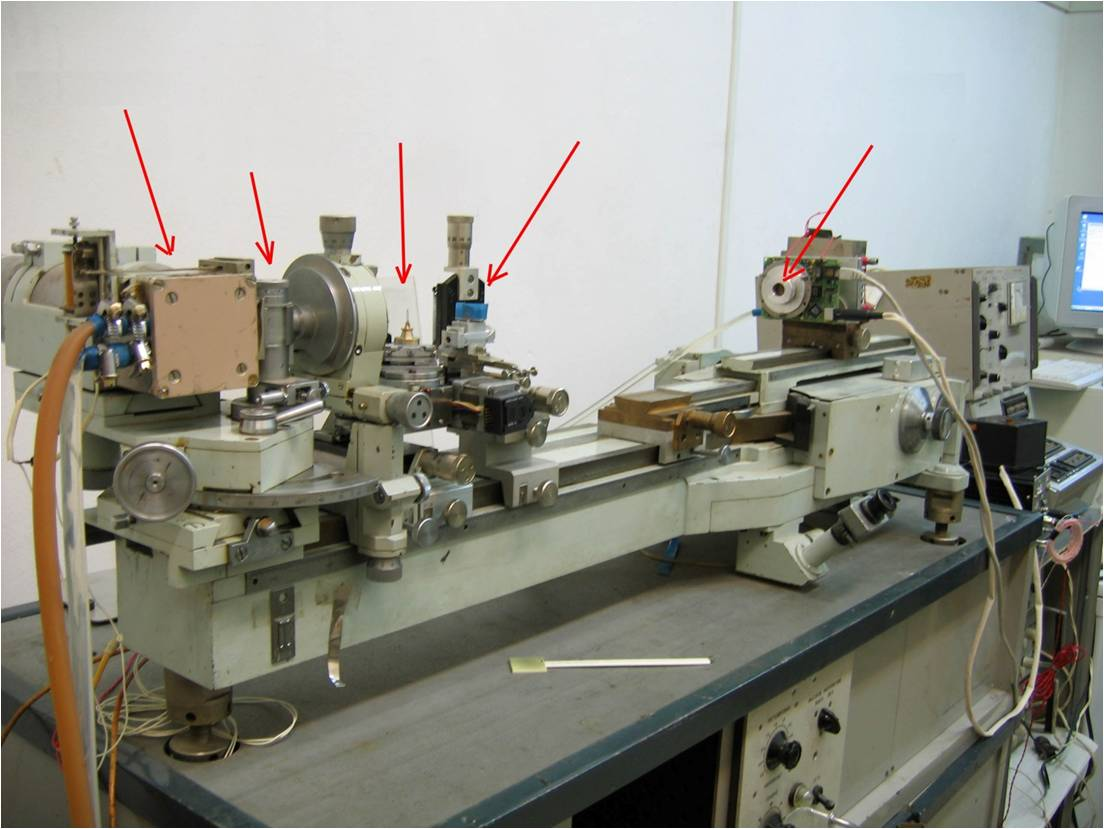
\includegraphics[width=0.7\textwidth]{intro_img/ct_scanner_CIRAS}
\caption{Один из ренгеновских томографов ИК РАН}
\end{figure}

Ренгеновское излучение источника, проходя через предварительные фильтры в виде монохроматора и \textbackslash или коллиматора, попадают на объект исследований.
Объект закреплен на вращающейся относительно источника платформе.
Ренгеновское излучение, проходя через объект, поглощается объектом, в результате чего интенсивность излучения ослабляется в соответствии с законом Бугера-Ламберта-Бера \cite{sivukhin_blb}:

\begin{equation}
\notag
I = I_0 \exp\left( {-\int \! f(l) \mathrm d l }\right),
\end{equation}

где $l$ ---  координата вдоль направления распространения луча, а $f(l)$ --- линейный коэффициент ослабления рентгеновского излучения, $I_0$ --- исходная интенсивность излучения источника, $I$ --- интенсивность излучения, попадающего на измерительный детектор, а интеграл берется вдоль прямой $l$.

Прошедшее через объект излучение регистрируется позиционно-чувствительным детектором.
После дискретизации отклика матрицы детектора даные поступают на обработку ПО реконструкции, которое восстанавливает линейный коэффициент ослабления по набору таких измерений объекта под разными углами проекции.
Для того, чтобы понять принцип работы алгоритмов реконструкции, нужно подробнее описать модель формирования измерений.
Рассмотрим в качестве примера схему эксперимента с параллельным пучком излучения.

\section{Измерения с параллельным пучком}
Несмотря на свою простоту, схема измерений 2D сечения объекта параллельным пучком рентгеновского излучения является ``ядром'' всех алгоритмов восстановления КТ и имеет много применений на практике.
В реальных экспериментальных схемах параллельный пучок рентгеновского излучения можно получить на синхротронах, в лабораторных условиях при использовании монохраматоров, а так же в результате пересчета измерений в веерной 2D геометрии, которая, в свою очередь, возникает в центральном сечении конуского пучка.
Параллельной формой может обладать только пучок монохроматического излучения. 

\begin{figure}[h!]
  \centering
  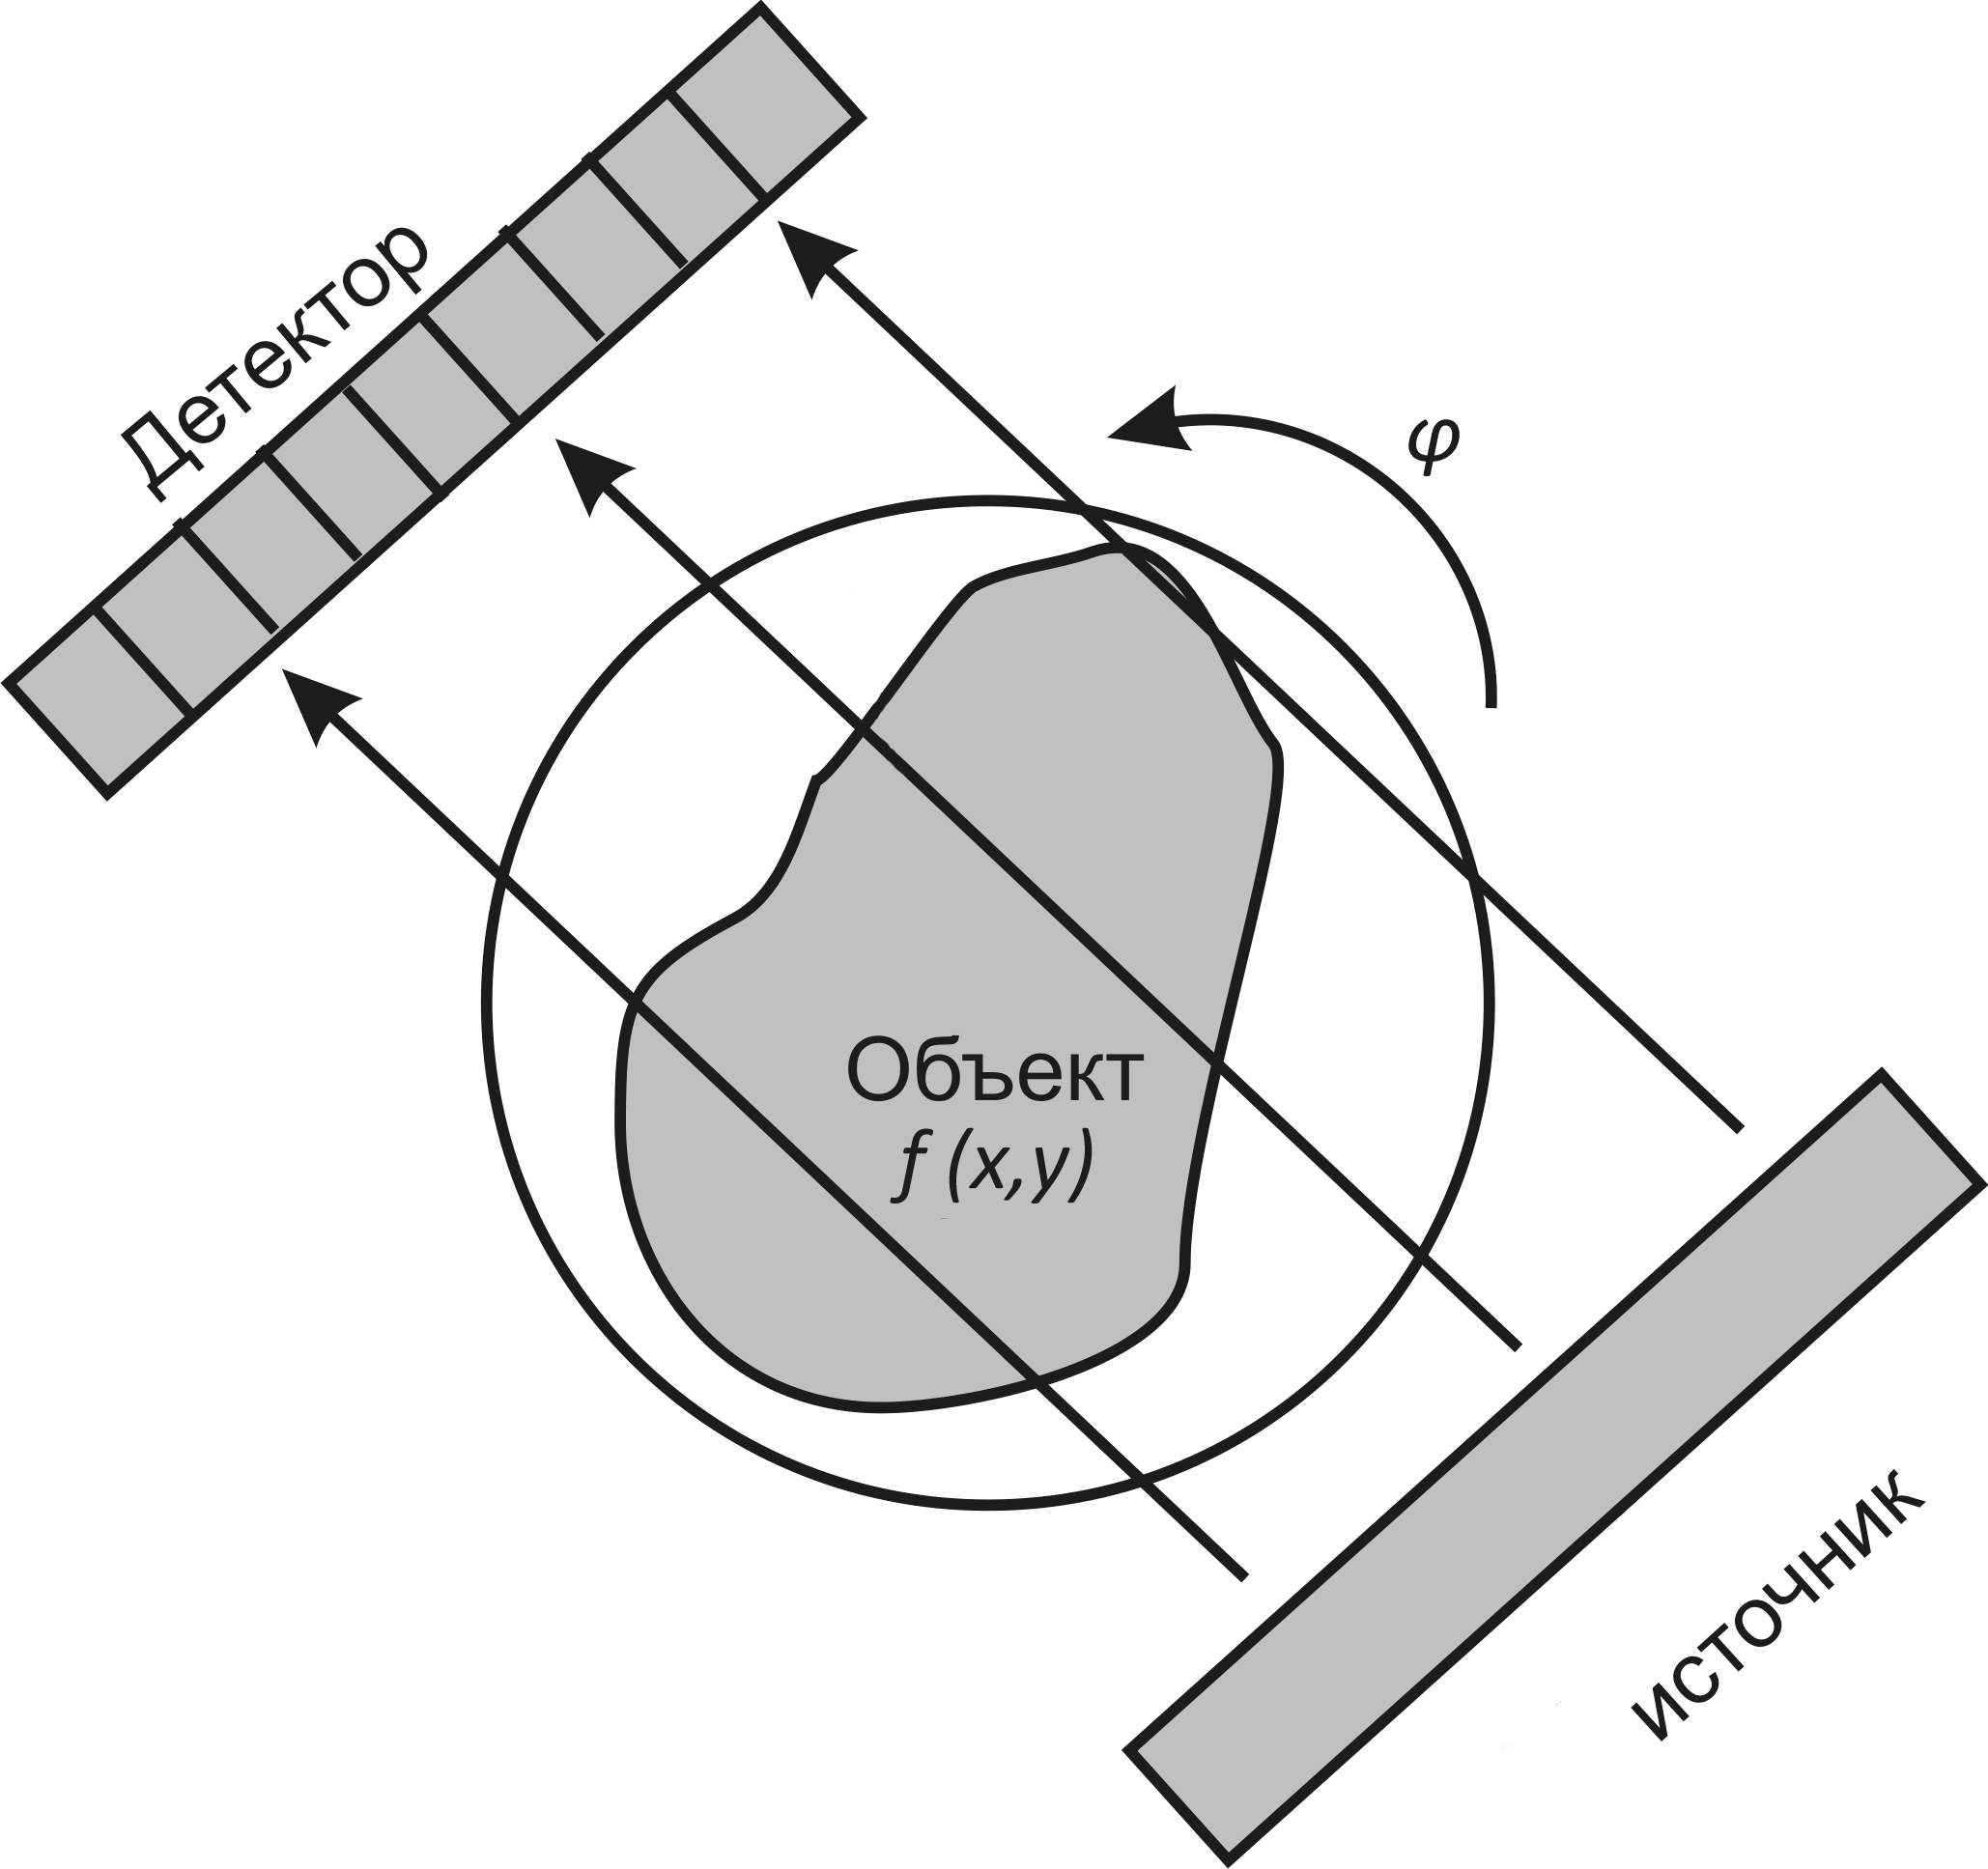
\includegraphics[width=0.5\textwidth]{part1_img/experiment}
  \caption{Схема измерений с параллельным пучком (2D)}
  \label{fig:experiment}
\end{figure}

Схема измерений изображена на рис. ~\ref{fig:experiment}.
Единичного измерения характеризуется двумя параметрами: углом поворота объекта и позицией ячейки детектора, к которой данное измерение относится.
Бесконечно тонкий рентгеновский луч, проходящий под углом $\varphi$  через объект на расстоянии $\xi$  от начала координат, описывается выражением
\begin{equation}\notag
  x\cos\varphi + y\sin\varphi = \xi.
\end{equation}
Тогда регистрируемый в пикселе детектора $\xi$ сигнал имеет интенсивность:
\begin{equation}\notag
  I(\varphi, \xi) = I_0 \exp\left( {-\iint \! \mathrm d x \mathrm d y f(x,y)\delta(x\cos\varphi + y\sin\varphi - \xi)}\right).
\end{equation}
Прологарифмировав обе стороны данного выражения, обозначаем измеренные данные как
\begin{equation}\notag
  p(\varphi, \xi) = \ln \left (\frac{I_0}{I(\varphi, \xi)} \right),
\end{equation}
получим преобразование Радона функции $R[f](\varphi, \xi)$:
\begin{equation}\notag
  p(\varphi, \xi)= \iint \! \mathrm d x \mathrm d y f(x,y)\delta(x\cos\varphi + y\sin\varphi - \xi) = R[f](\varphi, \xi).
\end{equation}
Суть задачи реконструкции в томографии --- восстановление двумерной функции сечения объекта ($f(x,\ y)$) по набору ее линейных интегралов вдоль конечного числа направлений, соответствующих проекционным углам, по набору проекций ($I(\varphi, \xi)$), или обращение преобразования Радона: $\hat{f}(x, y) = R^{-1}[p(\varphi, \xi)](x, y)$.

\section{Методы восстановления}
Задача восстановления изображения характеристики объекта по набору зарегистрированных проекций является задачей обращения преобразования Радона при условии конечного числа направлений проекции.
Существует два основных подхода к восстановлению измерений компьютерной томографии.

Первая группа методов --- интегральные \cite{herman2013mathematical, hsieh2009computed, zou2004exact, feldkamp1984practical}  --- подходит к решению задачи обращения преобразования Радона аналитически. 
Основной метод восстановления здесь --- метод свертки и обратной проекции (Filtered Backprojection, FBP) \cite{buzug2008computed}.
В основе этого метода лежит использование теоремы о центральном сечении, которая устанавливает связь между одномерным преобразование фурье от преобразования Радона по сдвигам $\hat{R[f](\cdot, \varphi)}$ и двумерным преобразованием фурье исходной функции $\hat{f}(u, v)$.
Для реконструкции искомой функции $f$ применяется явная формула обращения преобразования Радона:
$$
f(x,\ y) = \frac {1} {(2 \pi)^2} \int_0^\pi {
  \left(R[f](\dot,\ \varphi) * h\right)(x \cos \varphi + y \sin \varphi)
} \mathrm d \varphi
$$,
где $h$ это такая одномерная функция, что ее преобразование Фурье $\hat{h}(\omega) = |\omega|$, за $R[f](\dot,\ \varphi) * h$ обозначена свертка элементов преобразования радона для фиксированого угла $\varphi$ с этой функцией.
Именно из-за свертки с фильтром $h$ преобразования Радона метод получил свое название.
Применение FBP является стандартом де-факто в компьютерной томографии.
Вычислительная сложность этого метода определяется сложностью вычисления преобразования фурье изображения, т.е. $O(n^2 \log n)$.
Другой подход к выводу формулы обращения преобразования Радона, а так же анализа необходимого числа измерений, приводится в работах Вайнштейна, Орлова \cite{vainstein_orlov, orlov}.

Интегральный, или аналитический, подход работает с измерениями томографа как с непрерывной функцией, явно решая задачу восстановления.
Данная группа методов является вычислительно эффективной, однако может порождать некачественные востановления, содержащие высокий уровень шума и артефакты \cite{Lucas_sota_ir_survey_2015_radiology}.
Интегральные методы очень чувствительны к наличию шумов в иземенных данных, обоснованная плохой обусловленностью оператора обращения преобразования Радона. 
Так же эти методы требуют наличия большого количества проекционных углов и их равномерного распределения.
Интегральные методы не позволяют учесть априорных знаний о специфике восстанавливаемых объектов.

% дополнить описание FBP формулами

Вторая группа методов --- алгебраические \cite{algebraic_methods}. 
Алгебраические методы решают задачу восстановления распределения линейного коэффициента ослабления рентгеновского излучения в объекте в виде решения СЛАУ.
Уже на этапе моделирования происходит переход к дискретному представлению восстанавливаемой функции, то есть к растровому изображению.
Происходит переход от непрерывных функций $f(x,y), p(\varphi, \xi)$ к дискретным изображениям $f_{ij}, p_{kj}$.
Непрерывное преобразование Радона $R[f](\varphi, \xi)$ для дискретных изображений при конечном наборе углоа проекции принимает вид преобразования Хафа для прямых \cite{Ginkel04ashort}.
Если рассматривать изображения как конечномерные вектора в линейных пространствах размерностей $n \times n$ и $n_\varphi \times n$, то линейному преобразованию Хафа будет соответствовать некоторая матрица $W \in \mathrm{Mat}(\mathbb R, n n \times n_\varphi n)$.
Восстановление сводится к решению СЛАУ большой размерности $Wf = p$.

Первым алгоритмом из семейства алгебраических методов был ART (Algebraic Reconstruction Technique) \cite{GORDON1970471}, в котором авторы применили итерационный метод Качмажа (Kaczmarz) \cite{Kaczmarz1937} решения СЛАУ.
Сам метод Качмажа является частным случаем метода покоординатного спуска или, если речь идет о рандомизированной версии --- стохастического градиенты \cite{needell2014stochastic}.

В зависимости от типа градиентного спуска выделяют разные группы алгебраических методов: SART (Simultaneous Algebraic Reconstruction Technique) \cite{sart}, SIRT (Simultaneous Iterative Reconstruction Technique) \cite{GILBERTSIRT, gregor2008computational}.
В SIRT за один шаг обновления значения переменной используются значения по всем проекционным лучам, в ART --- по одному лучу, в SART --- по всем лучам одного угла проекции.
Введем обозначения: 

\begin{itemize}
	\item $W^{\mathrm T}_j$ --- строка матрицы Хафовской проекции $W$, отвечает за проекцию вдоль выделенной прямой $j$.
	\item $W^\varphi$ --- элемент декомпозиции проекции Хафа по углам. То есть умножение на эту матрицу дает элементы проекции по всем сдвигам но только для угла $\varphi$, а полная матрица $W = \sum W^\varphi$.
	\item $W^{\mathrm T}$ --- транспонированная матрица $W$. Ее умножение на элемент пространства проекций эквивалентен обратному проецированию (backprojection).
	\item $\gamma$ --- параметр релаксации
\end{itemize}

Тогда различия между одним шагом итерации методов ART, SART и SIRT будут выглядеть как это представлено в таблице \ref{tb:art_sart_sirt}:

\begin{table}[h]
\label{tb:art_sart_sirt}
\begin{tabular}{c|c|c}
ART & SART & SIRT \\ \hline
для каждого луча & для каждого угла & для всех лучей\\
$j = 1 \dots N * N_\varphi$ & $\varphi_k$ & \\
$\hat{f} = f - \gamma \mathrm W^{\mathrm T}_j(\mathrm W f - p)$ &
$\hat{f} = f - \gamma \mathrm {W^{\varphi_k}}^{\mathrm T}(\mathrm W f - p)$ &
$\hat{f} = f - \gamma \mathrm W^{\mathrm T}(\mathrm W f - p)$ \\
\end{tabular}
\\
\centering
\caption{Различия в шаге итерации у алгебраических методов}
\end{table}

Варьироваться в методах восстановления могут стратегии релаксации \cite{art_regparam} т.е. поведения $\gamma$ на каждом шаге, и перебора проекций \cite{art_pointschoice}, то есть порядка выбора $\varphi_k,\ j$.
Итеративная природа данных методов позволяет управлять процессом восстановления, используя регуляризацию и априорные знания об объекте исследования.
Так же одним из преимуществ алгебраических методов является довольно общая постановка задачи оптимизации, что позволяет использовать общие наработки теории итеративной градиентной оптимизации для улучшения качества восстановления и скорости сходимости алгоритма.
В последнее время  интерес к итерационной оптимизации особенно сильно возрос в связи с бурным развитием технологий обучения нейронных сетей \cite{battiti1992first, le2011optimization}.
В частности появляются адаптивные методы автоподбора величины шага градиента \cite{kingma2014adam, duchi2011adaptive, zeiler2012adadelta}, добавление затухания направления градиента \cite{qian1999momentum, nesterov1983method}.

Сравнения показывают, что алгебраические методы позволяют достичь лучшего качества восстановления \cite{sirt_less_artifacts, Lucas_sota_ir_survey_2015_radiology}.
В некоторых случаях, использование итерационных методов восстановления позволяет снизить дозу облучения на 70\% \cite{Willemink2013}, что особенно важно при применении томографии в медицине и биологии.
Так же встречаются гибридные методы, в которых итеративное применение интегрального восстановления используется для улучшения качества восстановленных картин.
Хотя концептуально алгебраические методы проще интегральных и лучше справляются с наличием высокого уровня шума в проекциях, они проигрывают последним по времени реконструкции.
Один из способов ускорить восстановление алгебраических методов --- применение распараллеливания на базе графических процессоров \cite{buz2011cuda, sirt_gpu}.
Несмотря на наличие эффективных реализаций на конкретных вычислительных архитектурах, для широкого распространения алгебраических методов необходима возможность их использования на изображениях высокого разрешения.
Речь идет об улучшении асимптотической сложности вычисления итерации алгебраического метода.
Сложность итерации обычных реализаций алгебраических подходов --- $O(n_\varphi n^2)$).
Необходимы асимптотически эффективные реализации как прямой, так и обратной томографической проекции.
Среди реализаций прямой проекции можно отметить так называемоем быстрое преобразование Хафа (БПХ), или дискретное преобразование Радона (ДПР) \cite{Brady1998, brady1992fast, hough, gotz1996fast}, сложность вычисления которого для изображения линейным размером $n$ --- $O(n^2 \log n)$.
Само преобразование было впервые опубликовано в работе Брейди 1992 года\cite{brady1992fast}, а потом независимо переоткрыто Готцом и Друкмюллером \cite{gotz1996fast}.
Позже в 2008 \cite{hough} преобразование вновь нашло применение в различных задачах компьютерного зрения и распознавания.
БПХ основано на использовании особого приближения лучей суммирования, называемого диадическими паттернами.
Оно определено для произвольных изображений в отличие от, например, предлагаемого дискретного преобразоваия Радона в \cite{Beylkin_DRT}, определенного только для периодических изображений.
Форма линии вдоль конкретной суммы получается в результате рекурсивной процедуры по размеру изображения, и отличается от традиционного Брезенхемовского приближения прямой.
Степень отклонения от реальных линий при использовании такого приближения подробно исследуется в работе \cite{ershov2015dyadic}.
Авторам удается теоретически подтвердить эмпирическое наблюдение \cite{Brady1998}, что в худшем случае отклонение диадического паттерна от идеальной линии не превышает $\frac 1 6 \log n$, где $n$ --- линейный размер изображения в пикселях.
Таким образом, при увеличении разрешения сканирования неточность приближения абсолютно тонкого луча в БПХ уменьшается с асимптотикой $O\left(\frac {\log n}{n}\right)$.
Авторы так же исследуют величину девиации трехмерного БПХ от идеальных плоскостей \cite{ershov3DHough}.
Говоря об эффективной версии обратной проекции можно отметить работу 2006 года \cite{Press_2006_invDRT}.
В ней предлагается искать обратное преобразование к БПХ с помощью рекурсивной процедуры путем приближения обратного преобразования, вычисленного на изображениях меньшего размера.
Неявно присутствует и описание вычисление градиента преобразования БПХ, которое так же является одним из результатов данной диссертационной работы.

\section{Наличие сильнопоглощающих включений}

Одна из известных проблем при востановлении измерений рентгеновской томографии --- возникновение артефактов, вызванных наличием металических (или других сильнопоглощающих) включений в структуре объекта \cite{barrett2004artifacts, boas2012ct, nasirudin2015reduction, park2015computed}.
Наблюдаемые искажения выглядят как темные полосы между металическими включениями со светлым полосатым ореолом окружающих тканей.
Столкнуться с такими артефактами можно, например, при медицинском сканировании пациента с металлическими коронками в зубах или костными протезами.
Наличие таких артефактов может затруднить нахождение или создать несуществующую патологию при медицинском анализе, скрыть или привнести трещины и полости при промышленных исследованиях.
Причины возникновения таких артефактов различны: ``огрубление луча'' (beam hardening), рассеяние, Пуассоновский шум, движение и краевые эффекты \cite{boas2012ct}.
Так же причиной возникновения таких артефактов является низкое соотношение сигнал-шум прошедшего излучения.
Чтобы избежать появления этих артефактов, используются различные методики: аппаратные, например, автоматическое управление модуляцие тока и напряжения на рентгеновской трубке, и программные, например, предобработка данных адаптивными фильтрами \cite{zhang2007reducing}.
Например, в \cite{boas2012ct} используется адаптивное расширение детектирующей ячейки в местах дефицита фотонов.
Еще одна группа методов использует измерения, полученные при зондировании различными энергиями \cite{bamberg2011metal, kuchenbecker2015dual}.

Есть методы, в которых модель формирования синограммы учитывается уже на этапе реконструкции.
Модифицированные алгебраические методы тоже используются для решения проблемы металлических артефактов: одни используют аппарат условной оптимизации при постановке задачи \cite{zhang2011metal, sidky2008image}, другие --- модифицируют целевую функцию \cite{meyer2010normalized, kotsenas2015ct}.
Хотя задачи условной оптимизации, возникающие при восстановлении, по сути являются задачами конического программирования второго порядка (SOCP) \cite{boyd2004convex, nesterov2009primal}, использование обычных алгоритмов для их решения, реализованных в программных комплексах выпуклого програмирования \cite{andersen2013cvxopt, mosek2010mosek} не представляется возможным из за огромной размерности задач.
Для решения этих задач приходится применять менее эффективные по сходмости но более вычислительно подходящие методы, такие как метод внутренней точки \cite{kim2007interior} или метод проекций на выпуклые множества (POCS) \cite{sidky2008image}.

Так же для уменьшения артефактов, вызванных металическими включенями используют статистические методы реконструкции \cite{jmuller2006, buzug2008computed}.
В отлчие от методов на основе свертки и обратной проекции, в таких методах есть возможность независимого взвешивания каждого проекционного луча.
Алгоритмы на основе метода максимального правдоподобия, такие как MLEM \cite{buzug2008computed, wang1996iterative} и его модифицированная версия $\lambda$-MLEM \cite{oehler2007statistical}, позволяют улучшить качество восстановленного изображения по сравнению с обычной линейной интерполяцией или предположением о пропущенных данных \cite{amirkhanov2012evaluation}.
Сравнение коммерчески доступных методов подавления артефактов \cite{huang2015evaluation} показывает, что эта проблема не является решенной в прикладных применениях компьютерной томографии, артефакты подавляются не полностью, и это активное поле для исследователей алгоритмов КТ.

\begin{comment}

\todo{введение - обзор из статьи аит2013 и бакалаврского диплома}

 Предлагаются новые версии алгоритмов, основанных на алгебраическом подходе, способных работать с сильно зашумлёнными проекциями. Такое условие сформировано необходимостью сокращать время регистрации проекций. Для некоторых применений уменьшение времени регистрации связано с требованием сокращения дозы облучения, для других --- обусловлено высокой динамикой поведения исследуемого объекта. Также следует отметить, что алгебраические методы реконструкции незаменимы, когда речь идет об экспериментах с малым числом проекционных углов и измерениях в ограниченном телесном угле. Только алгебраические методы применимы для решения задач трансмиссионно-эмиссионной томографии, если ослаблением зондирующего и вторичного излучений пренебречь нельзя.




\end{comment}

\section{Учет полихроматического спектра}
Решение задачи томографической реконструкции в условиях полихроматического сканирования \cite{Herman1979bh} до сегодняшнего дня остается актуальной проблемой, несмотря на большое количество исследований, которые ведутся в разных лабораториях мира.
Основные подходы, применяемые сегодня в методе компьютерной томографии, при работе с полихроматическим излучением --- использование двух различающихся спектров для зондирования \cite{graser2009dual, marin_2014_dual_energy_ct, kuchenbecker2015dual}, использование монохроматоров \cite{tan2012beam}, использование спектрально-чувствительных детекторов \cite{sidky2018three}, и особая обработка данных с томографа. 
В первом случае в 2 раза увеличивается радиационная нагрузка на объект исследования, что нежелательно при исследовании, например, живых объектов.
Во втором сильно уменьшается интенсивность исходного излучения.
Применение фильтров уменьшает поток квантов в единицу времени, что при ограниченном времени измерения снижает величину регистрируемого сигнала и, соответственно, повышает отношение шум/cигнал. 
Так же чтобы корректно провести фильтрацию, необходимо априорное знание об элементном составе образца, а оно не всегда доступно.

Остальные три подхода, это предобработка данных \cite{dewulf2012sense}, создание алгоритмов реконструкции, в которых полихроматичность заложена в математической модели, используемой при обратном проецировании, и постобработка восстановленных изображений. 
Пост процессинг восстановленного изображения \cite{krumm2008reducing} при использовании в ядре реконструкции полихроматической модели, не позволяет получить количественной информации о восстанавливаемом объекте, даже если визуальное представление сильно улучшается (в смысле показателей критериев, созданных для визуального контроля качества изображений).
Данный подход не может быть использован в таких областях применения компьютерной томографии, в которых от результатов КТ ждут количественной информации.
Это требуется в случаях, когда информация КТ не является конечной целью, а применяется при дальнейших расчетах и исследованиях.
Т.е. свойства исследуемых материалов должны быть описаны количественно.

Метод, предложенный в \cite{park2016metal} позволяет разделить металлические включения от биологических тканей в исследуемых образцах, при этом исправив артефакты восстановления, вызванные наличием этих включений.
Авторы пользуются явной формулой для вычисления коррекции на этапе пост-обработки, при этом производя оптимизацию ее гиперпараметров на этапе восстановления.
Одно из важных наблюдений авторов состоит в том, что немонохроматичность слабо проявляется в слабопоглощающих тканях, реальная зависимость от спектра присутствует только в металлических включениях.

Второй подход к решению задачи базируется на том, что модель, используемая при обратном проецировании, учитывает эффект полихроматичности.
При этом используются разные приближения \cite{stenner2010dynamic, van2011iterative}.
В работе \cite{brabant2012novel} детально описана процедура реконструкции, она легко применяется к модельным данным, показывает отличные результаты, однако, в ней опущен шаг перехода от нелинейной системы уравнений, которая описывает процесс формирования томографической проекции в полихроматических условиях, к линейной системе, которая потом решается с учетом полихроматичности.
Результаты предварительных исследований показали, что вопрос перехода от нелинейной системы к линейной не является тривиальным, а требует глубокого исследования и описания случаев, для которых при строго соблюденном перечне условий переход вообще является математически корректным.

Наконец, использование предобработки, т.е. коррекции зарегистрированных проекций перед шагом построения синограммы.
Его сильной стороной является тот факт, что если коррекцию удается провести с учетом поглощательных свойств всех включенных в исследуемый объект компонент, то затем можно применять методы реконструкции, созданные для монохроматического зондирования.
Для эффективной реализации такого способа коррекции необходимо создать базу параметров коррекции для типичных классов исследуемых образцов.
Такая база требует постоянного дополнения и перепроверки, с целью дополнительной калибровки корректирующих кривых.
И тем не менее, поскольку часто время реконструкции является важным параметром при создании программного обеспечения, такой процесс подготовки является приемлемым.    % Введение
\chapter{Вычислительно эффективный алгебраический метод восстановления FHT-SIRT} \label{chapt1}

\section{Введение}

В данной главе предложен и обсуждается асимптотически быстрый алгоритм SIRT \cite{GILBERTSIRT}, основанный на реализации быстрого преобразования Хафа (БПХ) \cite{hough}.
Алгоритм решает задачу восстановления для случая зондирования монохроматическим параллельным излучением.
Требуемое доказательство асимптотической оценки сложности алгоритма представлено.
Численная реализация алгоритма проиллюстрирована результатами реконструкции модельного изображения размером 256 $\times$ 256 по полному набору 1021 углов БПХ и по разреженным синограммам, имеющим до 11 раз меньшее число проекционных углов.

\section{Алгебраический подход}
Одна из отличительных особенностей алгебраического метода --- переход к дискретному представлению сущностей в задаче на в самом начале решения задачи. 
Дискретное представление изображения $\textbf f$ будет удобно обозначать с двумя индексациями: линейной ($f_j$) и матричной ($f_{kl}$). 
Матричная форма удобна для восприятия характеристики $\textbf f$ как двумерного изображения с пространственными значением координат.
Линейная форма же удобна при работе с изображением как с элементом линейного пространства.
Хотя существует множество способов отображения двумерных пространственных координат в одномерный индекс, конкретный способ линейной индексации не имеет значения в дальнейших выкладках.
Из соображений простоты и определенности, можно считать, что изображения-столбцы индексируются в порядке инексации матричных осей, т.е. по строкам слева-направо ($j = k * n + l$, при размере изображения $n$ и индексации, начинаемой с 1).

Радоновское проецирование дискретного изображения может быть представлено в виде действия линейного оператора
\begin{equation}\label{eq:linear_system}
\textbf p = W \textbf f,
\end{equation}
где $\textbf p$ --- прологарифмированная и отнормированная синограмма, $\textbf f$ --- искомое изображение, а элемент $w_{ij}$ матрицы $W$ соответствует вкладу $i$-го пикселя в $j$-ый луч.
Коэффициенты $0 \leq w_{ij} \leq 1$ могут задаваться по-разному, например так:
\begin{equation}
\label{eq:coeff}
w_{ij} = \frac{\text{Площадь пикселя $i$, перекрываемая лучом $j$}}{\text{площадь пикселя $i$}}
\end{equation}
Вид матрицы $W$ задает оператор проектирования, используемый при восстановлении.
От оператора проектирования зависит поведение алгоритма восстановления.

В дальнейшем изложении будет использовано разложение матрицы $W$ и проекционных данных $\textbf p$ на составляющие, соответствующие определенному углу:
\begin{equation} \notag
\begin{array}{l l}
w_{ij} = \sum_{h = 1}^{M_\varphi} {w_{ij}^{\varphi(h)}}, & \quad
p_i = \sum_{h = 1}^{M_\varphi} {p_i^{\varphi(h)}}.
\end{array}
\end{equation}
Здесь $M_\varphi$ ---  полное число проекционных углов в синограмме, а  $w_{ij}^{\varphi(h)}$ и $p_i^{\varphi(h)}$ учитывают только лучи, направленные по углу с номером $h$ (т. е. элементы, не относящиеся к углу $h$, равны нулю).

\section{Метод восстановления ART}
\label{ss:SART}
В алгебраическом методе (ART) изображение восстанавливается с помощью итерационного процесса:
\begin{enumerate}
\item{задается начальное приближение --- 2D кусочно-постоянная функция $\textbf f^{(0)}$ , которая описывает распределение коэффициента ослабления;}
\item{рассчитывается \textbf{одна} лучевая сумма вдоль одного из направлений $(W\textbf f)_i$, где $i$ --- индекс синограммы, соответствующий выбранному направлению;}
\item{отличие значения величины точки на проекции от рассчитанной величины лучевой суммы распределяется с учетом весовых коэффициентов между всеми пикселями, определившими направление, формируя добавку $(\textbf p - W \textbf f)_i$;}
\item{добавка, взвешенная релаксационным параметром \cite{art_regparam}, суммируется с текущим значением 2D кусочно-постоянной функции:
  \begin{equation} \label{eq:art_it}
\begin{array}{l l}
    \mathrm f^{(\text{нов})}_j = \mathrm f_j + \gamma w_{ij}\frac{(\textbf p - W \textbf f)_i}{\sqrt{\sum_k {w_{ik}^2}}}, & \quad j \in \overline{1, N},
\end{array}
  \end{equation}

где $N = M_s \cdot M_s$ --- полное количество пикселей в восстанавливаемом изображении, а $M_s$ --- полное количество сдвигов луча (полное количество делений линейного детектора).}
\end{enumerate}
Шаги 2 --- 4 повторяются для следующего выбранного направления. 
Итерация считается законченной, когда операция выполнена для всех направлений.
Новая итерация повторяет шаги 2 --- 4. Итерационная процедура заканчивается согласно выбранному критерию останова.
Схема перебора точек на проекциях может быть различной \cite{art_pointschoice}.  

Существуют разные вариации метода ART.
Для дальнейшего повествования потребуется метод SART, отличающийся от обычного ART тем, что на одной итерации невязка вычисляется сразу по всем точкам синограммы, а после этого в изображение вносится одна большая поправка.
Таким образом, итерационный процесс будет иметь вид
\begin{equation} \label{eq:sart_it_1}
  \textbf f^{(\text{нов})} = \textbf f + \gamma{W}^\mathrm{T}\frac{\textbf{p} - W \textbf f}{\sqrt{\sum_{i,j} {w_{ij}^2}}},
\end{equation}  
где за ${W}^\mathrm{T}$ обозначено транспонирование матрицы $W$.

\section{Геометрическое описание итерации}
Полезно представлять геометрически, что происходит с изображением при одном шаге алгоритмов ART и SART.
Если начальным приближением было абсолютно черное изображение ($\textbf f^{(0)} = 0$), то после одной итерации ART при суммировании (\ref{eq:art_it}) изменяются лишь пиксели, соответствовавшие некоторому лучу.
Результирующее изображение будет черным и будет содержать только одну полосу, причем яркость пикселей в этой полосе будет пропорциональна весам. 

При учете всей проекции по некоторому углу $\varphi$ результирующее изображение может быть получено следующим способом.
Рассмотрим некоторую строчку $h$ синограммы, соответствующую углу $h \leftrightarrow \varphi$. Введем обозначения: 
\begin{equation}\label{eq:misalligment}
\begin{array}{l l}
q^\varphi_l = (\textbf p - W \textbf f)_{hl},& \quad l \in \overline{1, M_s}, \\
r^\varphi_{kl} = q^\varphi_l, & \quad k,l \in \overline{1, M_s}.
\end{array}
\end{equation}
В этой формуле $q^\varphi_l$ --- строка длины $M_s$, соответствующая невязке синограммы по углу $\varphi$ на текущей итерации; $r^\varphi_{kl}$ --- изображение размера $M_s \cdot M_s$, постоянное вдоль столбцов, причем каждая строка этого изображения равна $q^\varphi_l$.
Все лучи, соответствующие одному углу, считаем пронумерованными в порядке их отступа вправо.
Чтобы получить финальную поправку на текущей итерации, нужно повернуть изображение $\textbf r^\varphi$ на угол $\varphi$ и прибавить к исходному, умножив предварительно на релаксационный параметр $\gamma$.
Обозначим описанную процедуру так:
\begin{equation}
\label{eq:geometric_sart_it}
\textbf f = \textbf f^{(0)} +\gamma\cdot\text{\textrm{повернуть}}(\textbf r^\varphi, \varphi).
\end{equation}
Сравнивая вид (\ref{eq:sart_it_1}) и (\ref{eq:geometric_sart_it}), можно заключить, что
\begin{equation}
\label{eq:alg_geom_conn}
{W^\varphi}^{\mathrm T}(\textbf p - W \textbf f) = \text{\textrm{повернуть}}( \textbf r^\varphi, \varphi).
\end{equation}

\section{Применение преобразования Хафа}
Принципиальное различие между интегральным и алгебраическим подходами к восстановлению в томографии состоит в следующем.
Результаты работы методов одинаковы --- дискретное изображение, соответствующее просвечиваемому объекту.
Однако алгоритмы, основанные на интегральном подходе, считают восстанавливаемую функцию непрерывной вплоть до этапа вычислений, а алгебраические методы работают с дискретным изображением (кусочно-постоянной функцией) уже на этапе постановки задачи.

Аналогично, было предложено пойти дальше и заменить модель, которая наилучшим образом приближает лучи с физической точки зрения, на модель дискретных симметричных лучей-ступенек, позволяющую производить быстрые вычисления.
Такое приближение известно как \textbf{быстрое преобразование Хафа}.

Быстрое преобразование Хафа (БПХ) изображения $\textbf f$ размера $n \cdot  m$ --- это изображение $\textbf p$ размера не более чем $2(n+m) \cdot (n+m)$, в каждой ячейке которого хранится сумма пикселей $\textbf f$ вдоль соответствующих лучей; по строкам располагаются суммы вдоль лучей с одинаковым углом наклона, а по столбцам --- с одинаковым отступом.
Преобразование Хафа является дискретным аналогом преобразования Радона (см. рис. \ref{fig:hough_radon}).

\begin{figure}[h!]
  \centering
    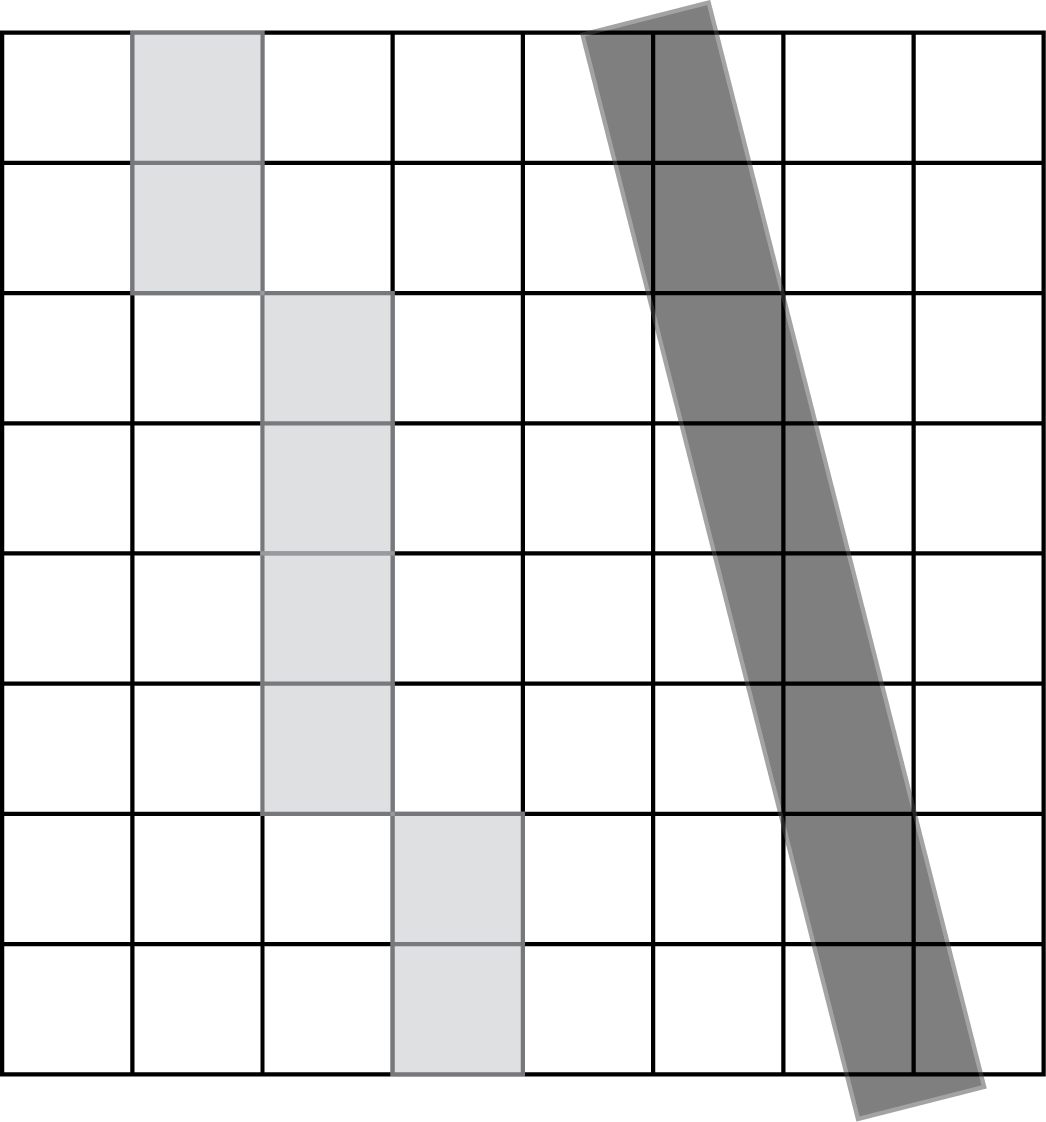
\includegraphics[width=0.55\textwidth]{part1_img/ART-Discr-ru}
 \caption{Различия в представлении лучей.}
Слева --- луч в БПХ, справа --- некоторе приближение бесконечно тонкого луча.
\label{fig:hough_radon}
\end{figure}

Полное преобразование Хафа изображения можно считать быстро за $O(n^2\log n)$, где $n$ --- линейный размер изображения.
Подробнее о быстром преобразовании Хафа можно прочитать в \cite{hough}.
Далее речь будет идти только о БПХ.

\section{Изменение в итерации}
Для построения алгоритма восстановления томографии, использующего преобразование Хафа в качестве оператора получения синограммы изображения, возьмем за основу алгоритм, описанный в разделе \ref{ss:SART}.
Полная накопленная поправка имеет вид
\begin{equation}
\label{eq:sum}
\Delta \textbf f = \sum_\varphi {{W^\varphi}^{\mathrm T}(\textbf p - W\textbf f) } = W^{\mathrm T}(\textbf p - W \textbf f).
\end{equation}
При использовании преобразования Хафа матрица $W$ становится заполненной только нулями и единицами в соответствии с паттернами углов, приближающих лучи.
Здесь и далее будем считать, что синограмма $\textbf p$ представлена в координатах пространства БПХ.
\subsection{Обоснование сходимости}
Рассмотрим функционал невязки
\begin{equation}
Q(\textbf f ) = ( W\textbf f - \textbf p)^2,
\end{equation}
где $W$ --- матрица весов.
Очевидно, что $Q( \hat{\textbf f}) = 0$, если $\hat{\textbf  f}$ --- восстанавливаемое изображение.
Найдем минимум функционала $Q$ методом градиентного спуска:
\begin{equation}
\nabla Q = 2 W^\mathrm{T}(W\textbf f - \textbf P).
\end{equation}
Шаг градиентного спуска выглядит так:
\begin{equation}
\label{eq:gradient_decay}
\textbf f^{(n)} = \textbf f^{(n-1)} - \gamma  W^\mathrm{T}(W\textbf f - \textbf p).
\end{equation}
Последнее уравнение соответствует итерационной процедуре (\ref{eq:sart_it_1}) с точностью до нормировки весовых коэффициентов.
%но это не имеет значения в случае использования преобразования Хафа, так как там нормы всех весовых коэффициентов одинаковы и могут быть включены в релаксационный параметр $\gamma$.

\subsection{Улучшение асимптотики}
Далее покажем, как улучшить асимптотику одной итерации с $O(n^3)$ до $O(n^2 \log n)$, где $n$ --- линейный размер изображения ($n = M_\varphi$).
% Здесь и далее векторное представление изображений не понадобится, но понадобится много индексов.
% Поэтому теперь индексация не всегда будет соответствовать использованной ранее в статье.

Так как понятие луча приобретает новое дискретное значение, понятие поворота тоже должно быть исправлено.
Чтобы сохранялось равенство (\ref{eq:alg_geom_conn}), повороты заменяются на \emph{скосы} в соответствии с паттернами скоса, отвечающими нужному углу.
\textbf{Паттерн скоса} для вертикального [горизонтального] направления $\varphi$ --- это массив длиной в высоту [ширину] изображения такой, что в каждом элементе записан сдвиг соответствующей строки [столбца]:
\begin{equation}\notag
\text{длина}(pattern_\varphi) = \text{высота[ширина]}(\textbf f),
\end{equation}
\begin{equation}\notag
pattern_\varphi[i] =\left\{
\begin{array}{c}
\mbox{ сдвиг $i$'ой строки [$i$'ого столбца] изображения \textbf f } \\ \mbox{ в пикселях при повороте на угол $\varphi$ }
\end{array}
\right\}.
\end{equation}


Рассмотрим в сумме (\ref{eq:sum}) только половину вертикальных углов (у которой нижняя точка правее верхней).
Полное количество этих углов $M_\varphi = M_s = n$.
$i$-я строка изображения $\Delta \textbf f$ --- сумма строк $\textbf q^\varphi$ (о которых говорилось в (\ref{eq:misalligment})), сдвинутых в соответствии с $pattern_\varphi[i]$, будет равна
\begin{equation}
\label{eq:sum_res}
\begin{array}{l l}
{\Delta f}_{ij} =  \sum_{k = 1}^{n} {q^{\varphi(k)}_{j + pattern_{\varphi(k)}[i]}} & \quad j \in \overline{0, \text{ширина}(\textbf f)}, \\
\end{array}
\end{equation}
Где $q^{\varphi(k)}_j$ определяется так:
\begin{equation} \notag
q^{\varphi(k)}_j = 
\begin{array}{l l}
\begin{cases}
0,& \text{если $j\leq0$ или $j > \text{ширина}(\textbf f)$;}\\
\frac{p_{kj} - \text{Хаф}(\textbf f)_{kj}}{\text{высота}^2(\textbf f)}, &\text{иначе.}
\end{cases}
\end{array}
\end{equation}
Здесь через $\text{Хаф}(\textbf f)$ обозначено преобразование Хафа от изображения.

Изображение $\textbf r = \frac{\textbf p - \text{Хаф}(\textbf f)}{\text{высота}^2(\textbf f)}$, где взята только половина вертикальных углов, будем использовать для подсчета суммы (\ref{eq:sum_res}).
Это изображение является, с одной стороны, частью невязки в пространстве синограмм, а с другой --- строками $q^{\varphi(k)}$, записанными друг под другом.

 Рассмотрим подробнее строку $i$ изображения $\text{Хаф}(\textbf r)$.
 Эта строка соответствует углу $\psi(i)$, а значит, и паттерну $pattern_{\psi(i)}$:
\begin{equation} \notag
\text{Хаф}(\textbf r)_{ij} =  \sum_{k = 1}^{n} {r^{\phi(k)}_{j + pattern_{\psi(i)}[k]}}
\end{equation}
\newtheorem{myth}{Теорема}
\begin{myth}
Пусть $pattern_j$ --- вертикальный паттерн скоса для j'ой строки преобразования Хафа изображения высотой $M_s = 2^n$.
Тогда имеет место равенство:
\begin{equation}
\label{statement1}
\begin{array}{l l}
pattern_j[i] = pattern_i[j] & \quad  i,j \in \overline{1, 2^n},
\end{array}
\end{equation}
т. е. матрица, составленная из паттернов скоса, записанных в качестве столбцов, симметрична.
\end{myth}
\begin{proof}
Так как соответствие между углами и строками преобразования Хафа взаимно однозначное ($\psi \leftrightarrow k$), то для краткости будем пользоваться только номерами строк.
Пусть $j = \overline{j_1 j_2 \dots j_n}$ --- двоичное представление числа $j$, т.е.
\begin{equation} \notag
j = 2^{n-1}j_1 + 2^{n-2}j_2 + \dots + j_n, j_k \in \{0,1\}.
\end{equation}

Исходя из процедуры нахождения паттернов скоса, число $\hat{j} = \overline{j_1 j_2 \dots j_{n-1}}$ соответствует паттерну ``предыдущего поколения''\, длиной $2^{n-1}$ (паттерн $j$ генерируется из двух паттернов, сдвинутых друг относительно друга на $pattern_{\hat{j}}[2^{n-1}] + j_n$ пикселей).
Легко видеть, что для любого $j$ длиной $2^n$ верно: $pattern_j[2^n] = j$ (см. рис. ~\ref{fig:patterns}).


\begin{figure}[h!]
  \centering
    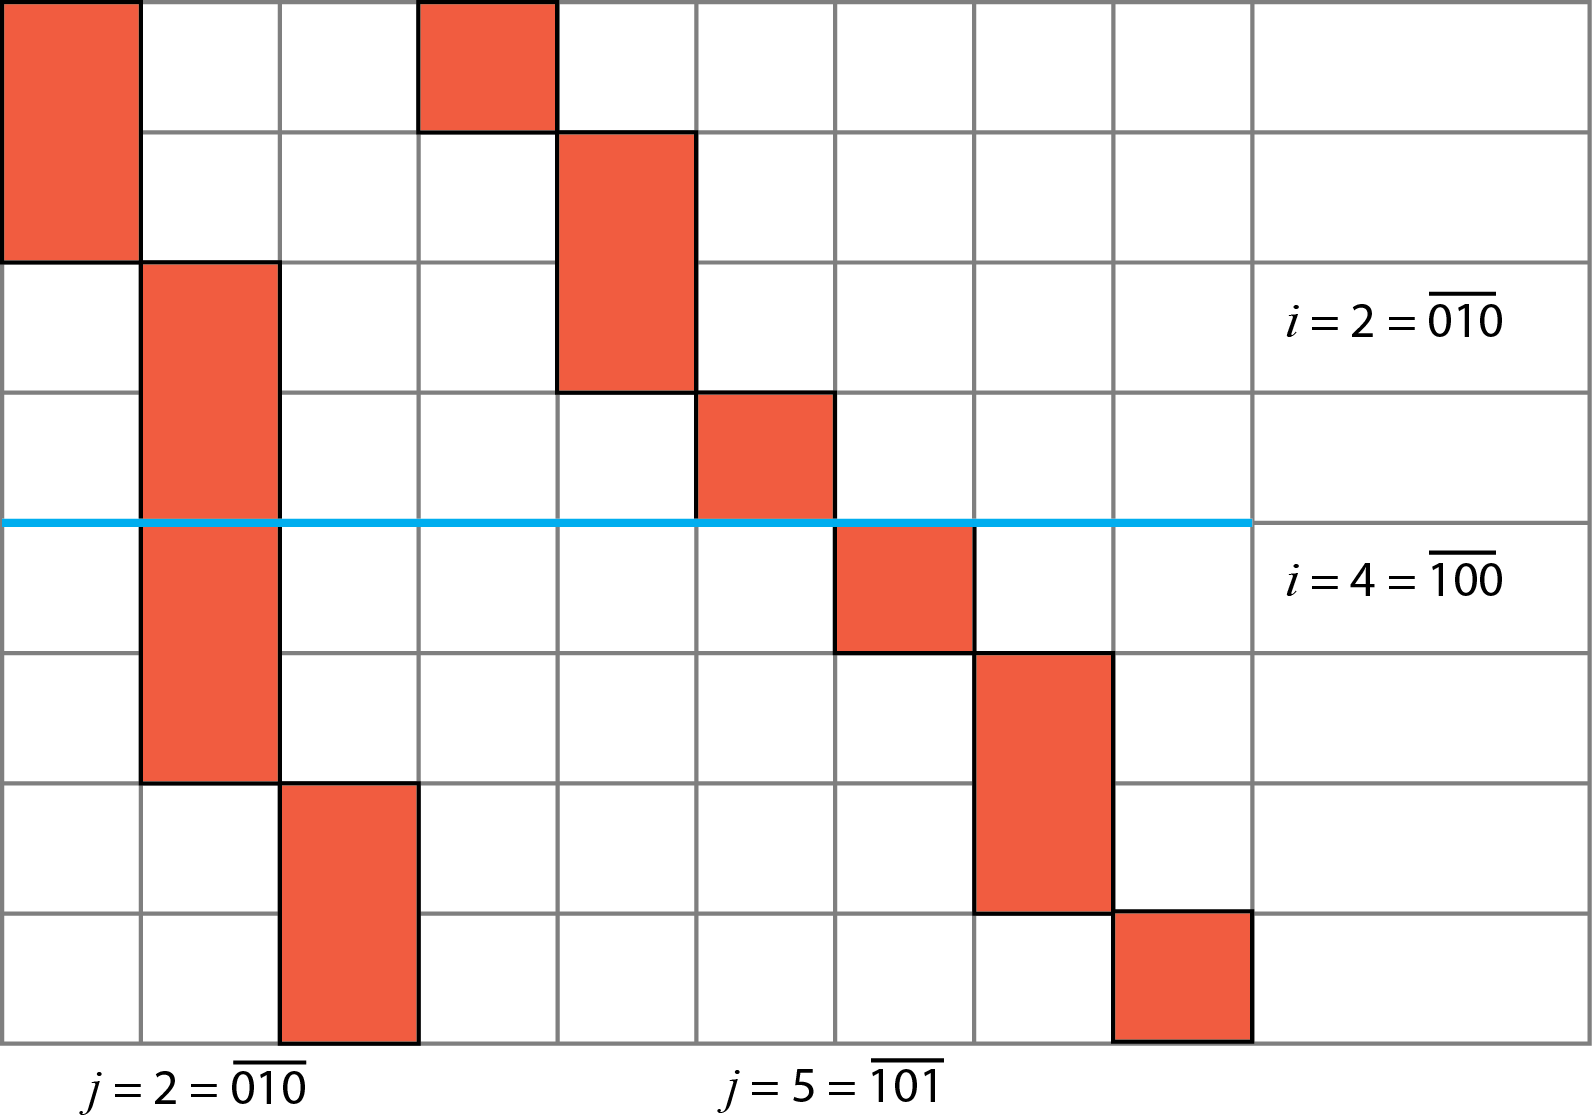
\includegraphics[width=0.7\textwidth]{part1_img/pattern_structure}
  \caption{Хафовские паттерны скоса.}
\label{fig:patterns}

Последняя цифра $j$ отвечает за наличие  дополнительного сдвига половинок на пиксель.
Первая цифра $i$ отвечает за выбор верхней или нижней частей.
\end{figure}

Теперь рассмотрим свойства двоичного представления другого индекса $i = \overline{i_1 i_2 \dots i_n}$, отвечающего номеру строки изображения, которую нужно сдвинуть.
Первая цифра $i_1$ показывает, меньше ли $i$ чем $2^{n-1}$, т. е. находится ли эта строка выше или ниже середины.
Если строка выше середины, то она соответствует верхней половине паттерна $j$, поэтому величина сдвига такая же, как для $\hat{j} = \overline{j_1\dots j_{n-1}}$ и $\tilde{i} = \overline{i_2\dots i_{n}}$.
Иначе величину сдвига нужно увеличить на $pattern_{\hat{j}}[2^{n-1}] + j_n = \hat{j} + j_n$ (см. рис. ~\ref{fig:patterns}):
\begin{equation}\notag
pattern_j[i] = 
\begin{cases}
pattern_{\hat{j}}[\tilde{i}], &\text{если $i_1 = 0$},\\
\hat{j} + j_n + pattern_{\hat{j}}[\tilde{i}], &\text{если $i_1 = 1$}.
\end{cases}
\end{equation}

Итак, можно написать, что:
\begin{equation}
\begin{aligned}\notag
pattern_j[i] = i_1(\hat{j} + j_n)+  pattern_{\hat{j}}[\tilde{i}] = \dots =\sum_{k = 1}^{n-1}{i_k\overline{j_1 j_2 \dots j_{n-k}}}\ +  \sum_{k = 1}^{n}{i_kj_{n-k+1}} =  \\ 
= \sum_{k = 1}^{n-1}{i_k(2^{n-k-1}j_1 + 2^{n-k-2}j_2 + \dots + j_{n-k})}+  \sum_{k = 1}^{n}{i_k j_{n-k+1}} = \\
= \sum_{k = 1}^{n-1}\sum_{m =1}^{n - k}{2^{n-k-m}i_kj_m} +  \sum_{k = 1}^{n}{i_kj_{n-k+1}}.
\end{aligned}
\end{equation}
Второе слагаемое, очевидно, симметрично относительно перестановки $i$ и $j$.
То же можно сказать и о первом слагаемом:
\begin{equation}\notag
\sum_{k = 1}^{n-1}\sum_{m =1}^{n - k}{2^{n-k-m}i_kj_m} = \sum_{\substack{k,m > 0 \\ k + m \leq n}}{2^{n-(k+m)}i_kj_m}.
\end{equation}
Показана истинность утверждения (\ref{statement1}), а значит, и теорема доказана.
\end{proof}

Итак, было показано, что вычислить поправку $\Delta \textbf f$ можно путем двух последовательных применений преобразования Хафа: сначала для вычисления невязки, а потом для вычисления суммы (\ref{eq:sum_res}).
Таким образом, сложность итерации оценивается как $O(n^2 \log n)$, где $n$ --- линейный размер восстанавливаемого изображения.

\section{Исследование поведения алгоритма}
На рис. ~\ref{fig:time_30it} изображена зависимость времени работы 30 итераций алгоритма, аппроксимированная функцией $C n^2 \log n$, при разных размерах изображения исходного фантома.

\begin{figure}[h!]
  \centering
    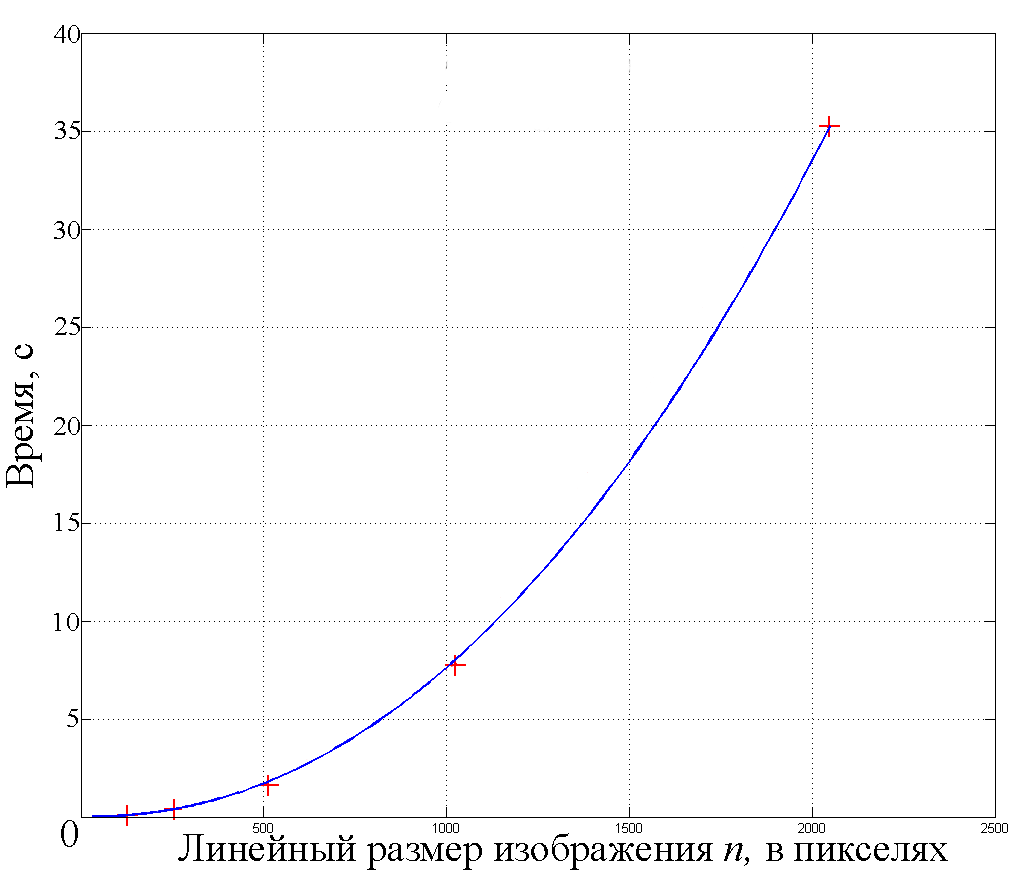
\includegraphics[width=0.7\textwidth]{part1_img/time_30_it}
  \caption{Время работы 30 итераций алгоритма.}
Линией изображена функция $Cn^2\log n$, крестами обозначено измеренное время работы.
\label{fig:time_30it}
\end{figure}

Было исследовано и количество итераций до достижения наперед заданной среднеквадратичной ошибки синограммы в зависимости от размера восстанавливаемого изображения (см. рис. \ref{fig:ris5},a).
Исследуемая величина уменьшается с увеличением размера, так как при большем размере изображения-фантома полное количество углов в БПХ становится больше, т. е. появляется возможность измерить более точную синограмму модели.

% \begin{figure}
% \begin{subfigure}[h]{0.45\textwidth}
%   \centering
%     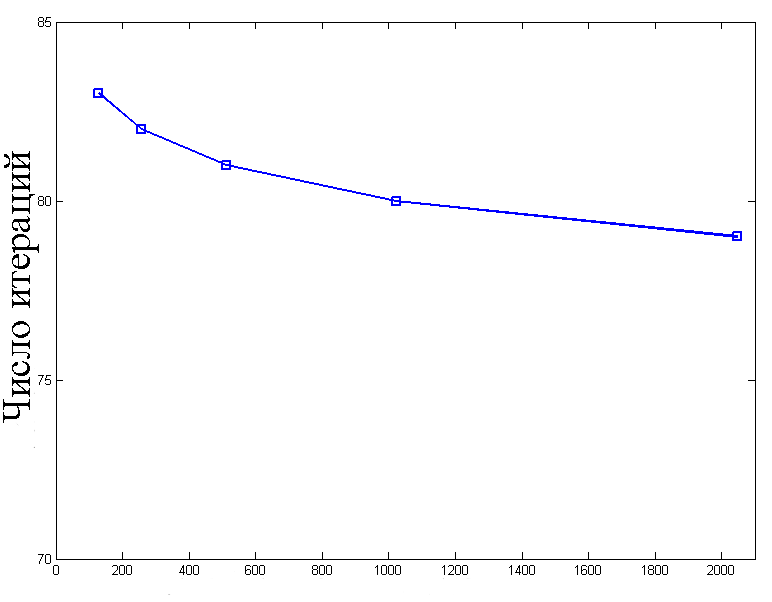
\includegraphics[width=\textwidth]{part1_img/it_till_stop}
%     Линейный размер изображения
% \label{fig:it_till_stop}
% \end{subfigure}
% 
% \begin{subfigure}[h]{0.45\textwidth}
%   \centering
%     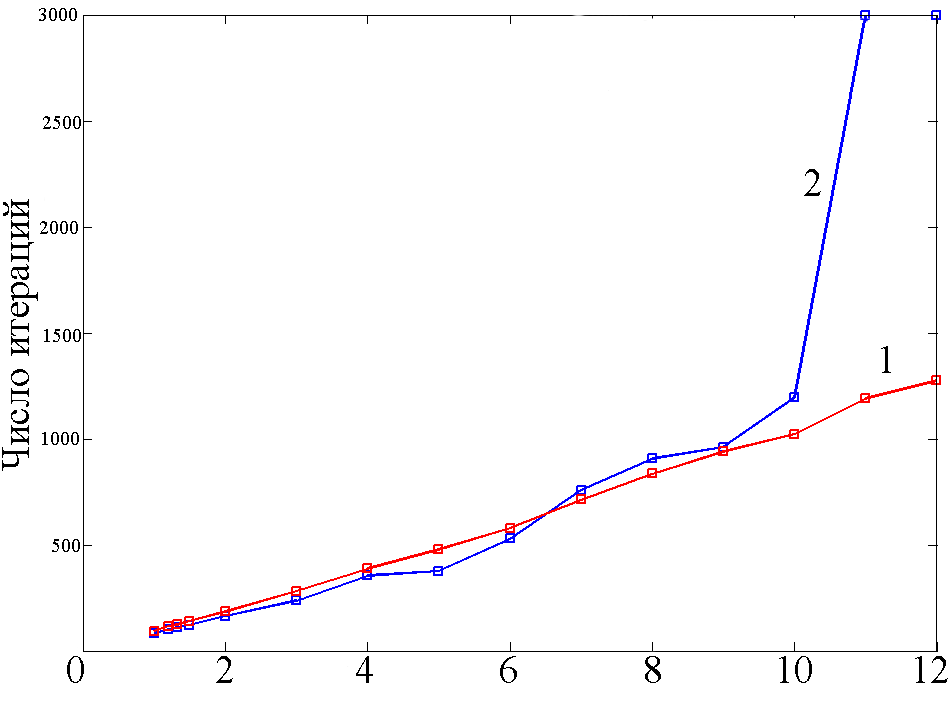
\includegraphics[width=\textwidth]{part1_img/median_correct}
%   Степень разрежения
% \label{fig:median_reg}
% \end{subfigure}
%   \caption{Количество итераций до останова.}
% \label{fig:ris5}
% \end{figure}

\begin{figure}
  \centering
\begin{tabular}{@{}c@{}c}
    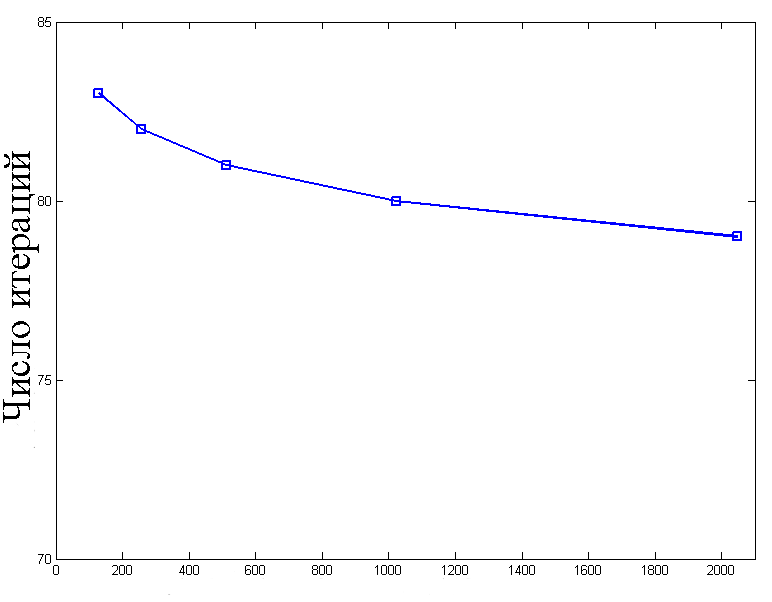
\includegraphics[width=0.45\textwidth]{part1_img/it_till_stop}
&
    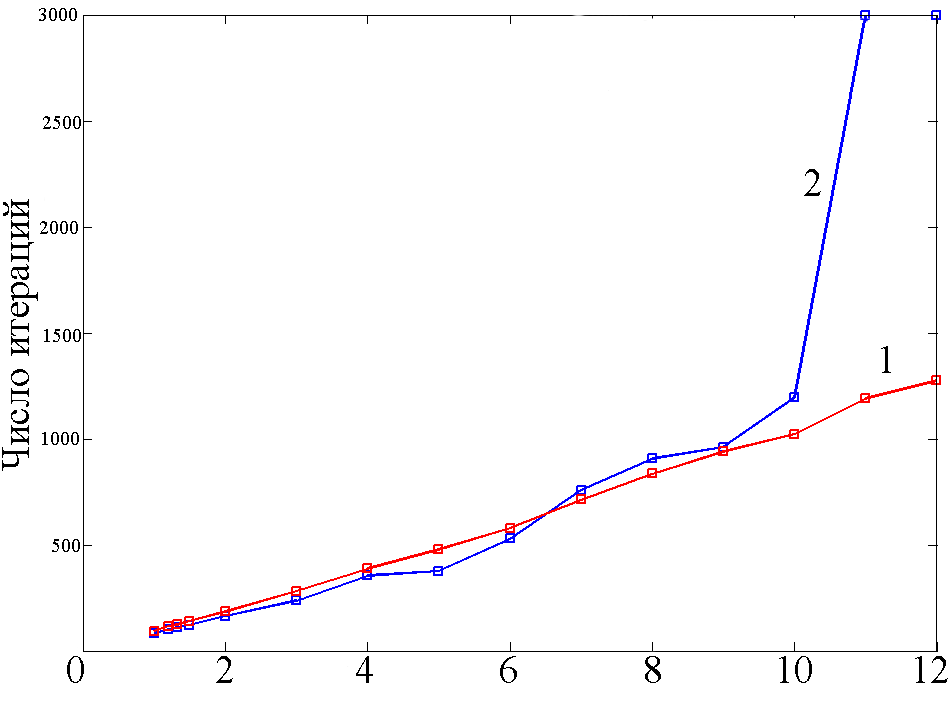
\includegraphics[width=0.45\textwidth]{part1_img/median_correct}
\\
    \small a) Линейный размер изображения    
&
    \small b) Степень разрежения
\end{tabular}
  \caption{Количество итераций до останова.}
\label{fig:ris5}
\end{figure}



Критерием останова в этом и в других экспериментах было достижение некоторой наперед заданной ошибки в преобразовании Хафа по среднеквадратичной метрике:

\begin{equation}\notag
\text{ошибка} = \frac{1}{M}\sum_{i = 1}^{M}{(p_i - \text{Хаф}(\textbf{f})_i)^2}.
\end{equation}

Рассмотренная зависимость была снята при наличии всех $4n-3$ проекций, т. е. полного преобразования Хафа.
В условиях реального эксперимента снять такое количество проекций не представляется возможным.
Действительно, уже для изображения $256\times 256$ пикселей потребовалось бы измерение $4n - 3 = 1021$ разных углов.
Поэтому при работе с реальными данными на входе алгоритма преобразование Хафа будет разреженным.
Время работы при этом останется таким же (в этом смылсе предлагаемый алгоритм проигрывает обычным алгебраическим методам).
Поэтому было исследовано поведение алгоритма при различном разрежении синограммы (см рис. \ref{fig:ris5},б).
На приведённых зависимостях степень разрежения $k$ означает, что для восстановления было использовано в $k$ раз меньше строчек, чем есть в БПХ.

\section{Регуляризация} \label{sect1_2}

При большом разрежении БПХ качество восстановления ухудшается --- недостаточность входных данных порождает шумы на восстановленной картине.
Для корректировки восстанавливаемого изображения применялась регуляризация --- сглаживающий фильтр с сохранением границ после каждой итерации.
Приведённые зависимости были сняты с использованием медианного фильтра размера $3 \times 3$ для изображения размером $256 \times 256$.
На рис. \ref{fig:ris5},б цифрой 1 обозначена зависимость с использованием медианного фильтра, цифрой 2 --- без.

Поведение итерационной процедуры при различном разрежении также отражают рис. \ref{fig:conv_all}.
На них изображено поведение логарифма среднеквадратичной ошибки восстанавливаемого изображения в пределах 5000 итераций.

\begin{equation}\notag
\text{ошибка} = \frac{1}{N}\sum_{j = 1}^{N}{(f^\text{фантом}_j - f_j)^2},
\end{equation}
где через $f^\text{фантом}_j$ обозначен пиксель идеального изображения, а через $f_j$ --- пиксель текущего.

%\begin{figure}
%\begin{subfigure}[h]{0.45\textwidth}
%\centering
%  \caption{}
%    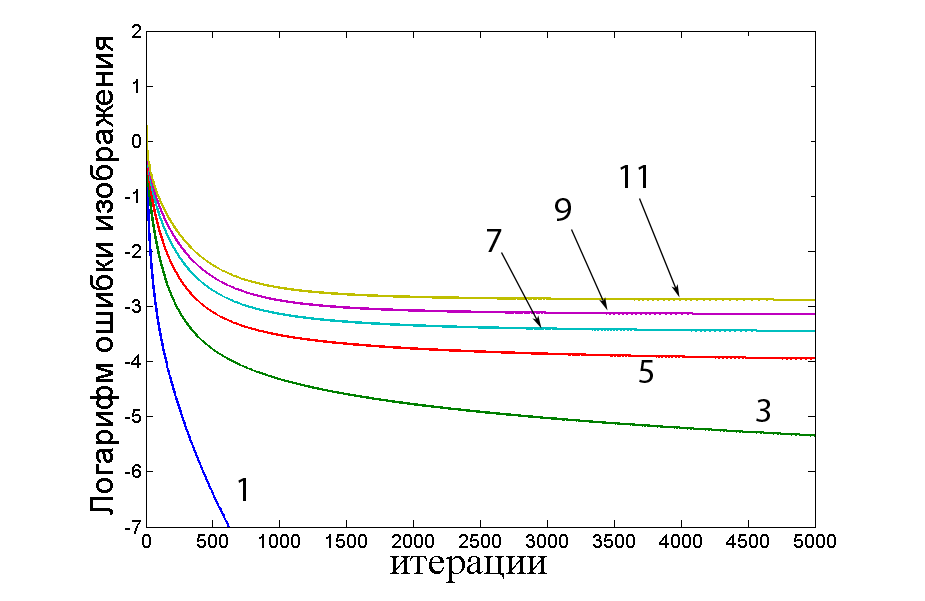
\includegraphics[width=\textwidth]{part1_img/raw}
%\label{fig:conv_raw}
%\end{subfigure}
%~
%\begin{subfigure}[h]{0.45\textwidth}
%  \centering
%  \caption{}
%    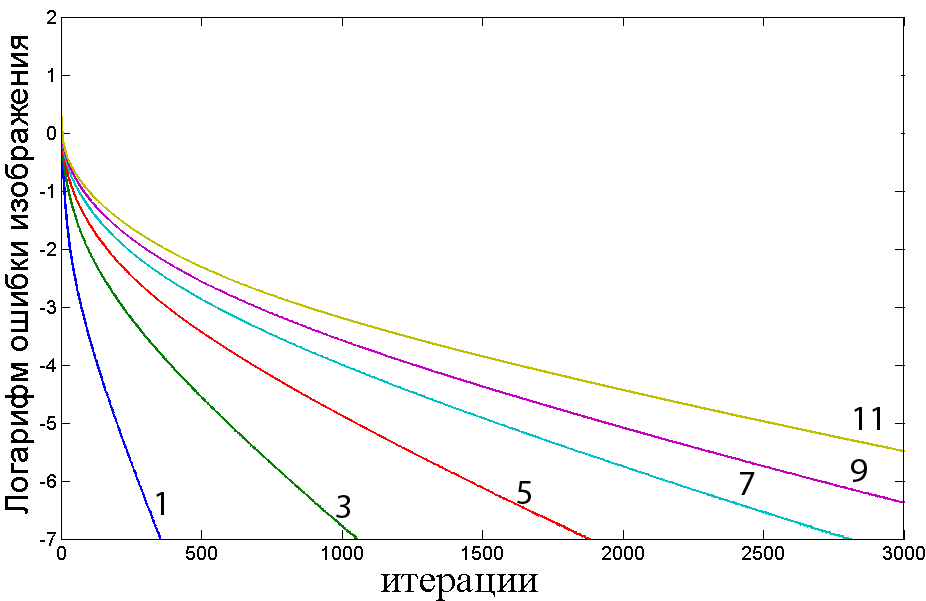
\includegraphics[width= \textwidth]{part1_img/medk}
%\label{fig:conv_med}
%\end{subfigure}
%  \caption{Зависимость среднеквадратичной ошибки изображения от числа итераций.}
%%  \centering
%Число рядом с кривой соответствует степени разрежения. а --- Без регуляризации, б --- Медианная регуляризация.
%\label{fig:conv_all}
%\end{figure}

\begin{figure}
\centering
\begin{tabular}{@{}c@{}c}
    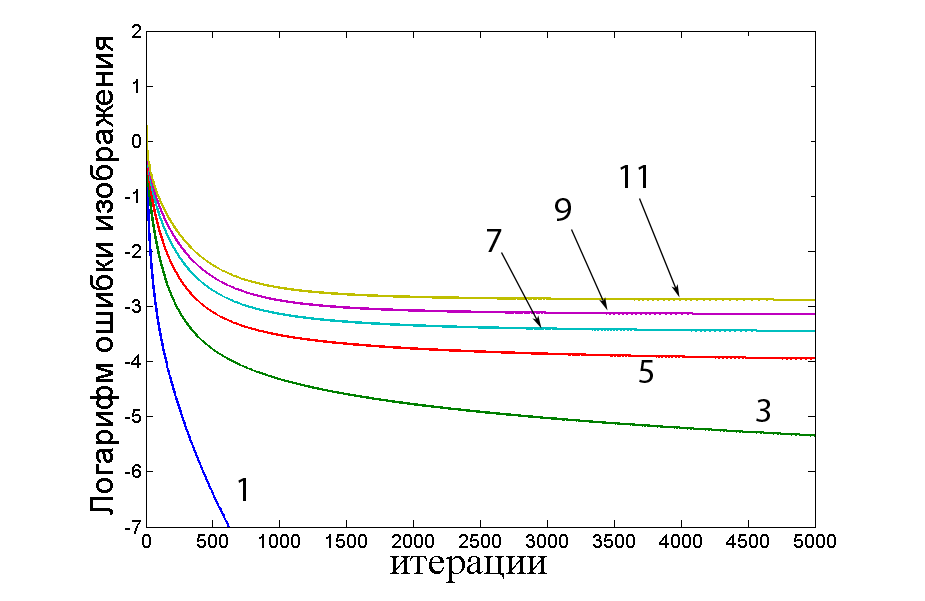
\includegraphics[width=0.45\textwidth]{part1_img/raw}
&
    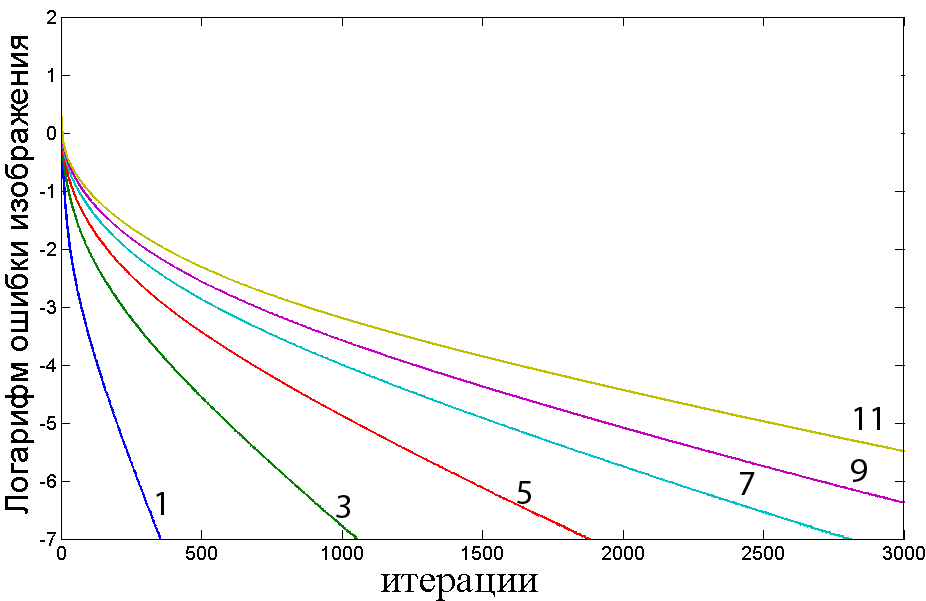
\includegraphics[width=0.45\textwidth]{part1_img/medk}
\\
   \small a) & \small b)
\end{tabular}
  \caption{Зависимость среднеквадратичной ошибки изображения от числа итераций.}
Число рядом с кривой соответствует степени разрежения. а --- Без регуляризации, б --- Медианная регуляризация.
\label{fig:conv_all}
\end{figure}


\section{Пространство проекции БПХ}
Данный раздел посвящен исследованию свойства пространства проекций вдоль дискретных лучей-ступенек, или БПХ-пространство. 
Помимо различий в точности приближения реального преобразования Радона, сама структура изображений БПХ, т.е. соответствие пикселей лучам проецирования, имеет особый вид.
Например, плотность хафовских лучей (по сдвигу) неоднородна отностиельно угла поворота.
Можно сказать, что хафовское приближение радоновского луча имеет свойсто утолщаться при приближении к углам, кратным $\frac \pi 4$.
Так же нуждается в дополнительном пояснении само соответствие Хафовской строчки углу проекции.
Изучение свойств пространства Хафа и его соотношение с реальными радоновскими координатами проекции необходимы, чтобы было возможно использовать алгоритм для работы с реальными данными экспериментов, а не только с имитированными хафовскими синограммами фантомов.

\todo{зависимость угла от строки Хафа (найти исходники заметки)}
\todo{зависимость количества сдвигов от угла}

\section{Переход к данным экспериментальных измерений}
\todo{восстановления реальных имеренных зубов хафовским алгоритмом, нормировка по косинусу.}
\todo{вставить текст статьи в Кристаллографию-2013}
\todo{вставить текст исследований про регуляризацию по Тихонову}

\todo{..исследовать L1, L0-регуляризаторы..?}

\section{Выводы}
В главе рассмотрена модификация алгебраического метода восстановления компьютерной томографии.
С помощью использования приближения бесконечно тонких рентгеновских лучей для дискретного изображения удается применить быстрое преобразование Хафа (БПХ) в качестве оператора генерации лучевых сумм.
Доказана возможность использовать БПХ не только для подсчета невязки преобразования Хафа, но и для вычисления поправки к изображению в итерационной схеме.
Последнее означает, что асимптотическое время, требуемое для вычисления одной итерации алгебраического метода, можно снизить, применив БПХ, с $O(n^3)$ до $O(n^2 \log n)$ от линейного размера изображения.

Представлены результаты численных экспериментов, описывающие поведение алгоритма в различных условиях.
Для недостаточно полных или зашумленных данных исследована возможность применения регуляризации.
Среди опробованных регуляризаторов на симуляциях сравниваются: медианный и билатеральный фильтры на этапе постобрбаотки и каждой итерации, $L_2$ регуляризация по Тихонову.
Приводятся характер поведения ошибки восстановления на модельных данных от количества итераций и параметров регуляризаторов.
           % Глава 1
\chapter{Подавление артефактов, вызванных наличием сильнопоглощающих включений} \label{chapt2}
\section{Причины возникновения артефактов}
\label{sect_2_0}
Здесь надо подробно описать используему модель возникновения артефактов из-за сильнопоглощающих включений.
Причина этому - количество фотонов, проходящих через металлические вставки, недостаточно для возбуждения электронов на чувствительном элементе детектора (на матрице).
В резульате измерения в этих пикселях детектора записаны как 0, то есть излучение сюда не пришло.
В реальности же, по этому 0 можно сказать только лишь то, что излучения туда пришло меньше чем порог активации пикселя.
Таким образом, в пикселях с 0 значением пришедшей энергии правильно ввести ограничения-неравенства.
При этом если использовать алгебраический подход, мы получаем задачу условной квадратичной минимизации, или квадратичного программирования.

\section{Компьютерная томография как задача квадратичного программирования} \label{sect_2_1}

Для решения этой задачи предлагается использовать численную реализацию алгоритма interior-point-convex из MATLAB (quadprog) \todo{найти нормальну ссылку на алгоритм и матлаб}

\section{Описание образца} \label{sect_2_1_1}
\begin{figure}
  \centering
  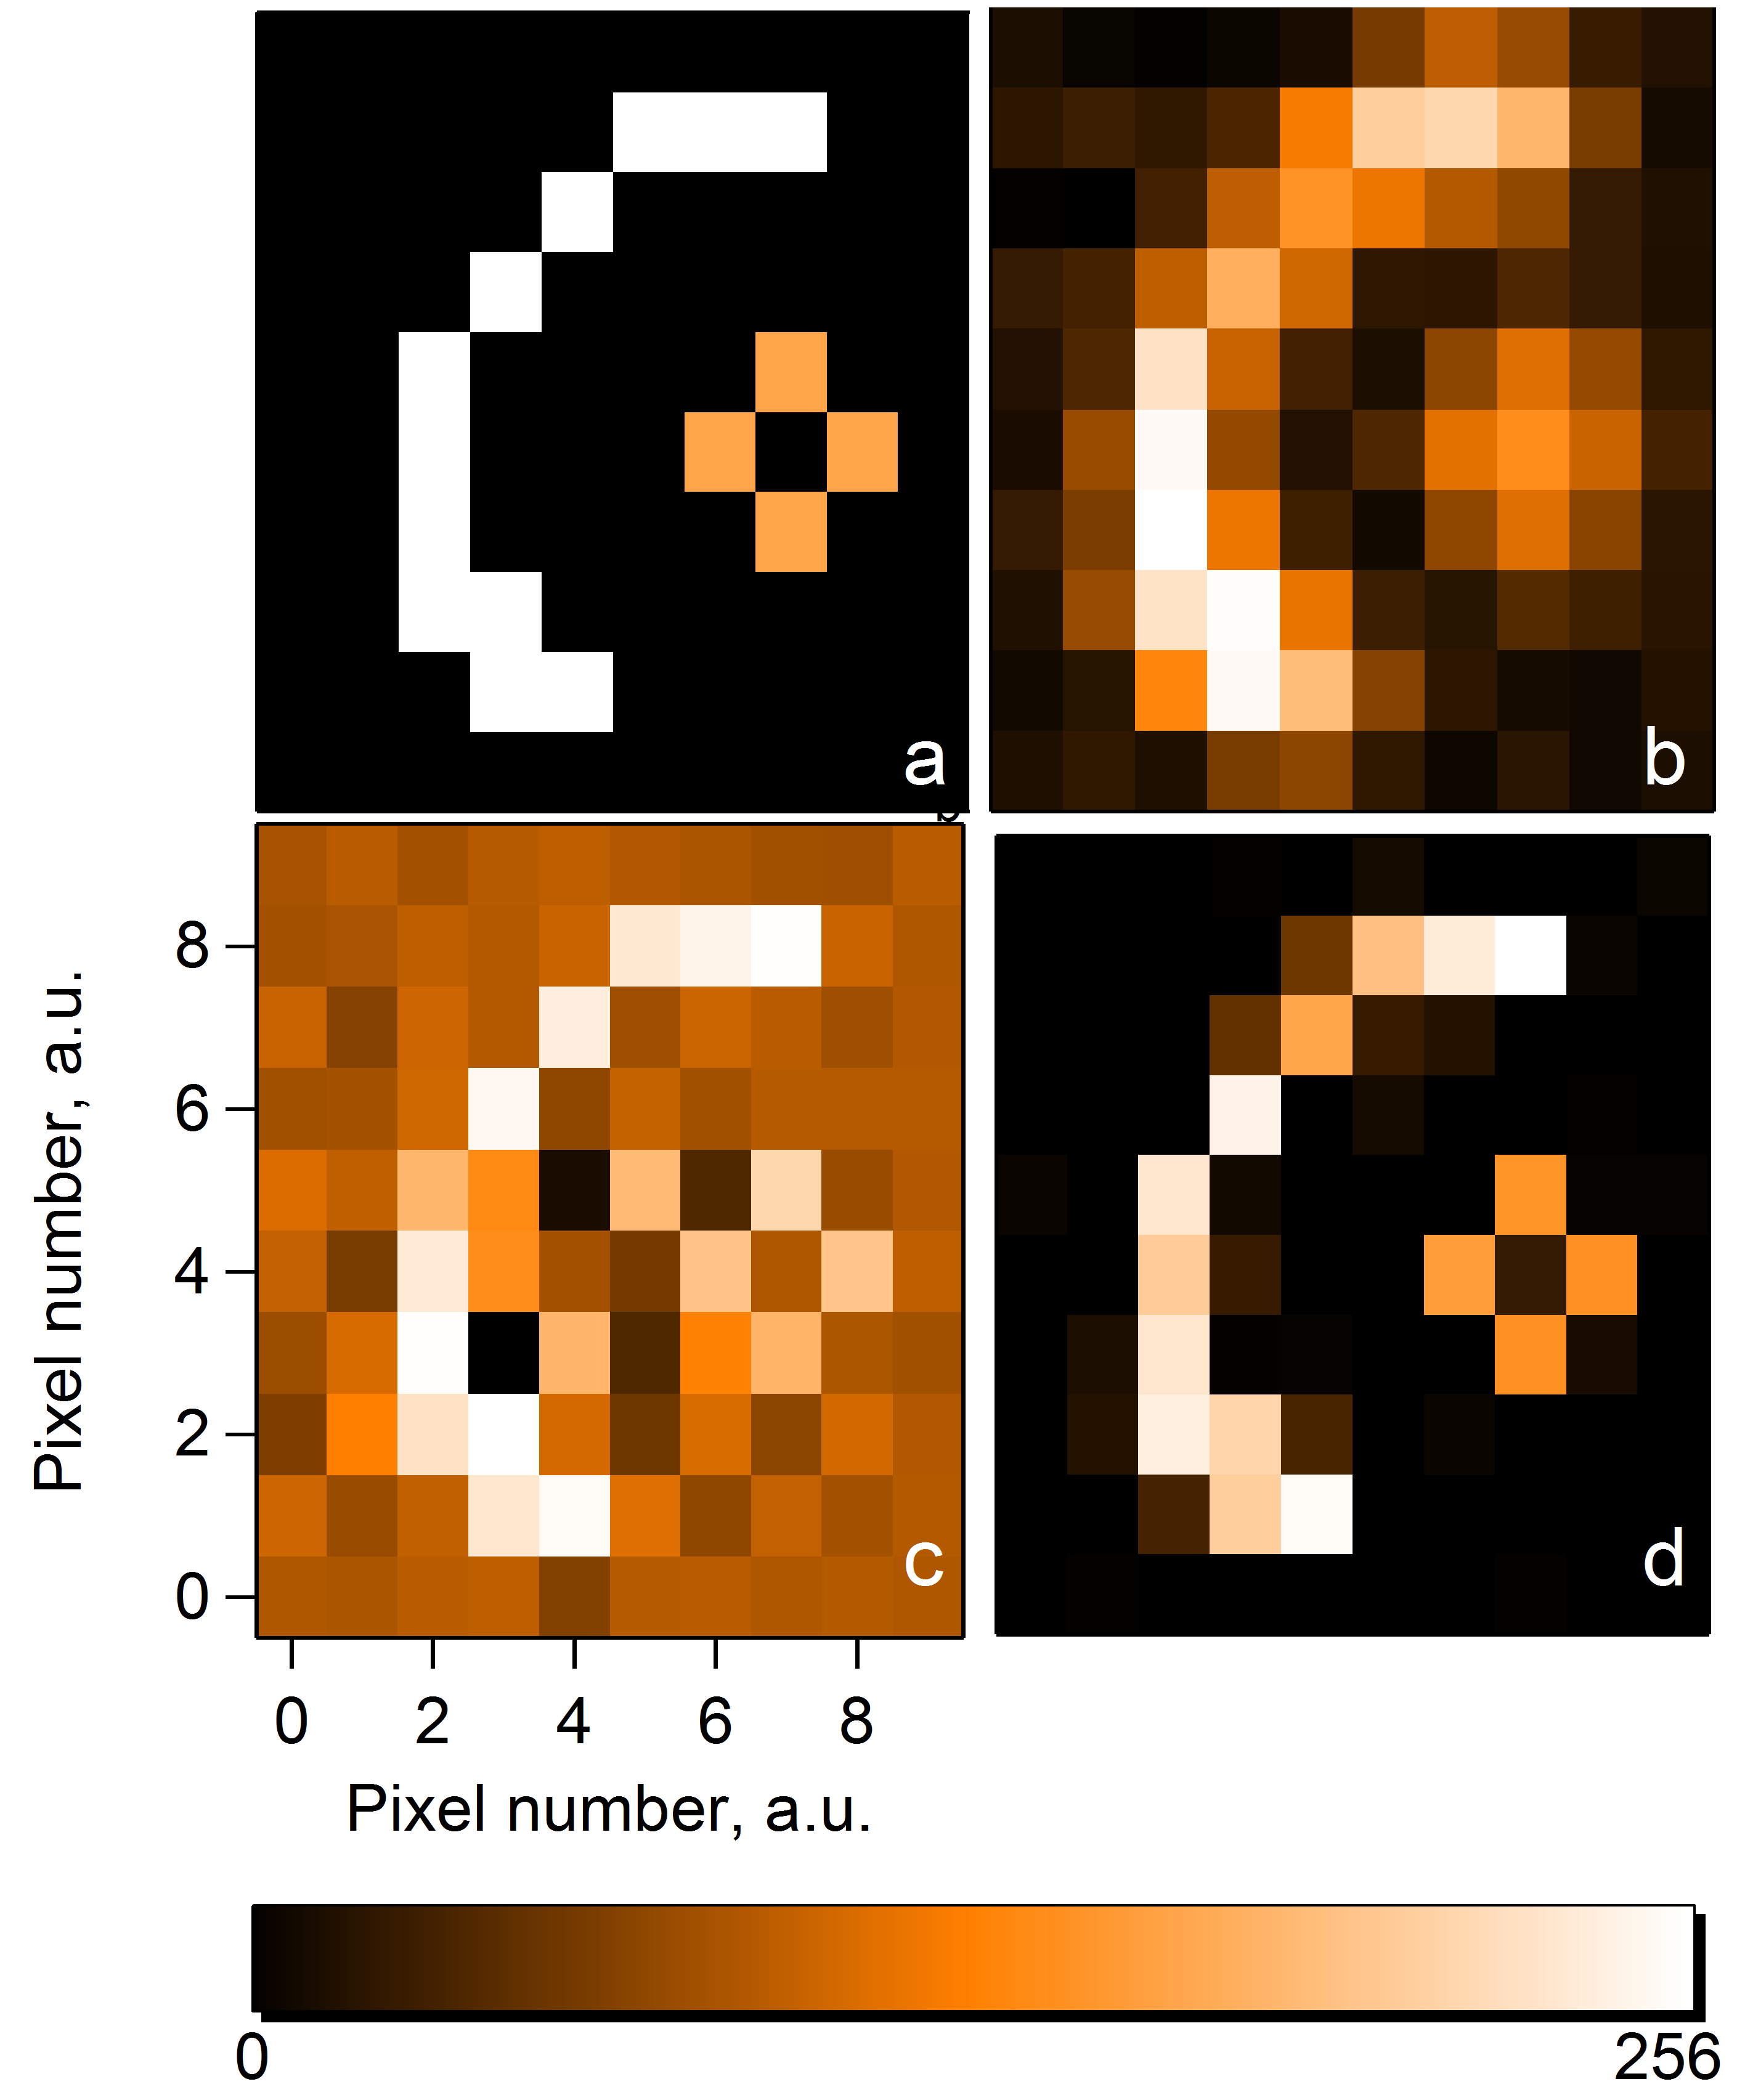
\includegraphics[width=0.7\textwidth]{part2_img/quadprog}
  \caption{Слева сверху - фантом использовавшийся для симуляций. Справа сверху - результат восстановления FBP. Слева снизу - результат восстановления квадратичным программированием без ограничений-неравенств. Справа снизу - результат восстановление квадратичным программированием с ограничениями-неравенствами (предложенный метод)}
  \label{im:quadprog}
\end{figure}

Для симуляции использовался фантом, изображенный на рисунке \ref{im:quadprog}a).
Это распределение вещества в сечении 10х10 пикселей, состоящее из двух объектов: скобки с высоким коэффициентом поглощения и крестика с нормальным уровнем поглощения.
Сгенерированная синограмма обрезалась по заданному значению порога, эмитируя эффект металлических включений.
Таким образом, была расчитана матрица проекции $\omega$, такая, что проеция $P = \omega \mu$ происходила по закону:

\begin{equation}
\label{eq:quadprog_projection}
P_j = 
\begin{cases}
\sum_i \mu_{i}\omega_{ij} , & \mbox{если} \mu_{i}\omega_{ij} < \mbox{порог} \\
\mbox{порог}, & \mbox{иначе}
\end{cases}
\end{equation}

, где $i$ - номер пикселя распределения, $j$ - номер луче проекции, порог подбирался таким образом, чтобы обрезать максимумы синограммы.
Значение порога было = 800, размер пикселя был 1х1.
Значение сильнопоглощающего включение было 256.
При расчете синограммы использовалось 35 проецкионых углов, равномерно распределенных в интервале от 0 до 180 градусов.

\todo{вставить синограмму}

На рисунке \ref{im:quadprog}b представлено восстановление полученной синограммы методом свертки и обратной проекции. 
Целью данного подраздела является улучшение данного восстановения методом квадратичного программирования.

Задача квадратичного программирования для воссатновления компьютерной томографии может быть сформулирована как 

\begin{equation}
  \label{eq:quadprog_eq}
  \begin{cases}
  \Norm{P^{\textup{изм.}} - P(\mu)} \rightarrow \min_{\mu} & w.r.t \\
  \sum_i \mu_{i} \omega_{ij} = P_j, & j = 1 \dots 35
  \end{cases}
\end{equation}

То есть условная минимизация с ограничениями типа равенства.
Результаты восстановления с помощью решения задачи (\ref{eq:quadprog_eq}) представлены на рисунке \ref{im:quadprog}с.

Следующим шагом в развитии этого метода восстановления является учет ограничений типа неравенства (\ref{eq:quadprog_projection}), учитывающих эффект сильного поглощения металлов.
задача (\ref{eq:quadprog_eq}) переходит в следующую:
\begin{equation}
  \label{eq:quadprog_ineq}
  \begin{cases}
  \Norm{P^{\textup{изм.}} - P(\mu)} \rightarrow \min_{\mu} & w.r.t \\
  \sum_i \mu_{i} \omega_{ij} = P_j, & \mbox{если} P^{\textup{изм.}}_j < \mbox{порог} \\
  \sum_i \mu_{i} \omega_{ij} > \mbox{порог}, & \mbox{если} P^{\textup{изм.}}_j = \mbox{порог}
  \end{cases}
\end{equation}

Восстановление с помощью решения (\ref{eq:quadprog_ineq}) изображено на рисунке \ref{im:quadprog}d.
Для восстановления использовался метод \cite{quadprog_algo}.
Как видно из рисунка, квадратичное программирование с условиями неравенствами обеспечивает лучшее восстановление границ и интенсивностей исходного фантома. 
Значения интенсивностей на разных частях восстановленых фантомов приведены в таблице \ref{tb:quadprog_res}:

\begin{table}[h]
\label{tb:quadprog_res}
\centering
\begin{tabular}{ r| c| c| c| c|}
 & \ref{im:quadprog}a & \ref{im:quadprog}b & \ref{im:quadprog}c & \ref{im:quadprog}d \\ \hline
скобка & $255 \pm 0$ & $146 \pm 25$ & $233 \pm 30$ & $225 \pm 26$ \\ \hline
крест & $164 \pm 0$ & $69 \pm 3.6$ & $170 \pm 19.5$ & $151 \pm 5.2$ \\ \hline
\end{tabular}
\caption{Средние значения и стандартное отклонение интенсивностей в разных областях исследуемого фантома}
\end{table}

Так же можно заметить, что использование квадратичного программирование с ограничениями типа неравенство обеспечивет лучшие значения интенсивностей с меньшим значением отклонения.


\section{Результаты} \label{sect_2_1_2}

\todo{текст ECMS\_2015}

\section{Мягкие ограничения на неравенства} \label{sect_2_2}

In this paper, we improve the results achieved in \cite{chukalinaway}. First, we provide a robust to noise and admissible to efficient optimization methods way to express the inequalities introduced in \cite{chukalinaway}. Second, we evaluate the method's performance on a simulated phantom data. The phantom data was simulated to remind a teeth with a metal object. And finally we evaluate the gain we get using the information in the inequalities against not using it at all.

The sections are organized as follows. Section \ref{s-approach} outlines the detail our approach to solve the problem. In Section \ref{s-phantom} the simulated phantom is presented. The obtained results are discussed in Section \ref{s-results}. Section \ref{s-conclusion} then concludes the whole paper.

% \section{Описание подхода}
\label{s-approach}
Let us denote the distribution of the attenuation coefficient in the reconstructed volume with $x \in \mathbb{R}^m$. The $p \in \mathbb{R}^n$ denotes the projection data detected during a scan. According to Beer-Lambert law the energy, detected at the detector cell, corresponding to $i$-th ray is expressed by the formula $p_i = I_0 * \exp(-a_i^T x)$, where $I_0$ is the source intensity, and $a_i$ is the row of the projection matrix $A$ corresponding to the $i$-th ray. A standard approach to find $x$ from the projection data is to take a logarithm and solve the linear system of equations: $Ax = r$, where
$r_i = \log(I_0) - \log(p_i)$. A standard way to get robust to noise reconstruction here is to use linear least squares:
\begin{equation} \label{eq:lls}
  \Norm{Ax - r}^2 \to \min\limits_{x}.
\end{equation}

Metal streak artifacts are caused mainly by photon starvation and noise. Mathematically it corresponds to the rays where $p_i$ is small or even zero. In latter case the logarithm is not defined and the simples way is just to ignore those rays solving instead of \eqref{eq:lls}:
\begin{equation}
  \label{eq:mask-lls}
  \Norm{P(Ax - r)}^2 \to \min\limits_{x},
\end{equation}
where matrix $P$ takes only those coordinates of a vector, at which $p_i \neq 0$. More precisely,
$$
P_{i,j} = \begin{cases}
  1, \quad\text{if $i = j$ and $p_i > 0$} \\
  0, \quad\text{otherwise}
  \end{cases}.
$$

It was suggested in \cite{chukalinaway} that even such problematic rays provide us with some information, namely that the weighted sum along such a ray has lower bound $a_i^T x > B$, for some suitable value of $B$ (for example, $B = \log I_0$), and we can use this information in a form of linear inequality constraints, solving the linear system with linear least squares approach:
\begin{equation}
  ||P(Ax - r)||^2 \to \min\limits_x, \quad\textrm{s.t. }  QAx \ge B,
\end{equation}
where $Q$ takes only those coordinates of a vector at which $p_i = 0$, opposite to the matrix $P$. Basically, $Q = E - P$, where $E$ is identity matrix.

This constraints being mathematically correct, are tight and are not robust against the noise in the projection data. Instead of tight constraints we propuse to use a soft version provided with a quadratic penalty method \cite{nocedal2006numerical} instead:
\begin{equation}
  \label{eq:soft-ineq}
  ||P(Ax - r)||^2 + \alpha ||[QAx - B]^-||^2 \to \min\limits_x,
\end{equation}
where $[y]^- = \min\{0, y\}$.

This functional provides a soft way to enforce the inequalities on the variables, but also allows to handle noise effects more smoothly. We can regulate the effect of that smoothing by manipulating $\alpha$: the greater $\alpha$ is tighter the effect of inequalities is.

The objective function \eqref{eq:soft-ineq} is convex and differentiable. We can effectively minimize it with Conjugate Gratient method (we used the implementation of this method, provided by the Python package \cite{scipy}). To speed-up computation of forward and backward tomographic projection operators we used ASTRA Toolbox \cite{palenstijn2011performance, van2015astra} which performs efficient evaluation of such operators on GPU.
\begin{figure}[h]
  \centering
  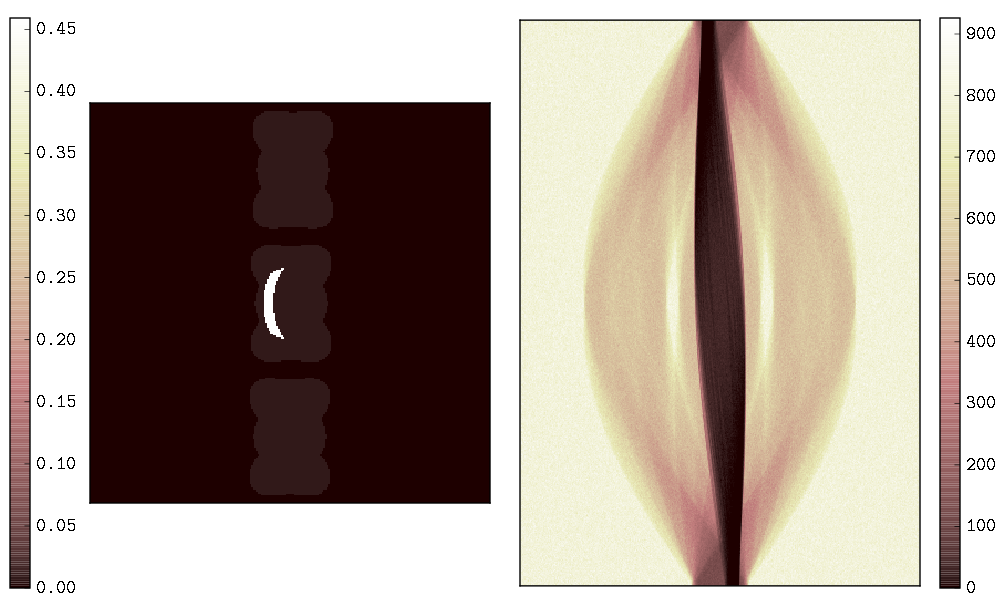
\includegraphics[scale=0.45]{part2_img/phantom-and-projection}
  \caption{The phantom (left) and its projection at $I_0 = 10^3$ photons (right).}
  \label{phantom-and-projection}
\end{figure}

\section{Описание образца}
\label{s-phantom}
To simulate the sinogram in $55$keV monochromatic mode we used a phantom imitating three teeth. Middle tooth contains titanium include imitating an implant (fig. \ref{phantom-and-projection}, left image). Pixel size is $0.005$cm. 2D field view size is $256 \times 256$ pixels. We used the XRayLib library \cite{brunetti2004library, schoonjans2011xraylib} to calculate the X-ray attenuation in each pixel for chosen energy. The sinogram (fig. \ref{phantom-and-projection}, right image) was calculated in a parallel scheme. We used $512$ rotation angles uniformly distributed in the interval $[0, \pi)$. The number of the detector cells is $362$, so that the diagonal of the phantom is projected on the detector without loosing any information. Such geometry choice allowed us to ignore the uniqueness of the solution issues which are related to the null-space of the projection operator and are ususally dealt with some sort of regularization techniques.

\section{Результаты}
\label{s-results}
To study the proposed approach we generated projections for different source intensities and draw several samples of Poisson noise at each source intensity.

For each projection we reconstructed the volume using Missing Data Least Squares \eqref{eq:mask-lss} and proposed Soft Inequalities Least Squares \eqref{eq:soft-ineq} approaches. The value of $\alpha$ was chosen to be equal to $50$.. The reconstructed volume was then compared to the original phantom and Mean Square Error was compute for such a pair.

In the figure \ref{sample} we can see an example of such reconstructions. In absence of the information encoded in the inequalities the metal artifacts are presented and there is a strong shadow in the cental tooth, while in the left image, reconstructed with Soft Inequalities approach those artifacts are significantly reduced.
\begin{figure}
  \centering
  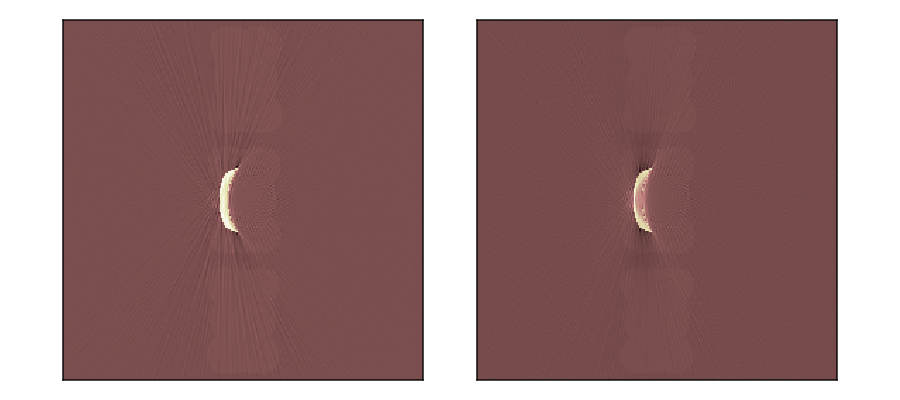
\includegraphics[scale=0.5]{part2_img/sample}
  \caption{Example of reconstruction with Soft Inequalities method (left)
    and Missing Data method (right).}
  \label{sample}
\end{figure}
In the figure \ref{error-plot} we can see the plot of MSE averaged over all the samples of noise for each noise level. The inequalities provide an improvement over ignoring such data at all noise levels.
\begin{figure}
  \centering
  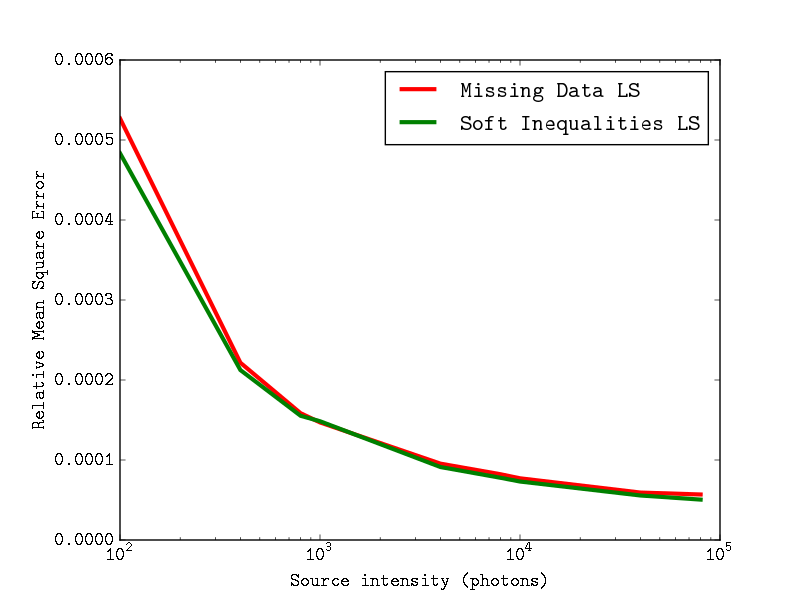
\includegraphics[scale=0.5]{part2_img/error-plot}
  \caption{The MSE value with respect to noise level.}
  \label{error-plot}
\end{figure}

\section{Выводы}
\label{s-conclusion}

Experiments shows that the information encoded in the inequalites, introduced in \cite{chukalinaway} carries a significant information which can be used to reduce metal-like artifacts in the reconstructions. We proposed a robust way to use this information in form of panaltized objective function. The proposed functional is suitable to be minimized with an efficient numerical algorithms enabling the approach to work on mid- and large-sized data. Proved to work, the method next should be deeper with respect to sensitivity to $\alpha$ and compared against the other approaches mentioned in the introduction. It is also seems possible to leave the penalty encoding the inequality constraints, replacing the least squares functional with more statistically suitable (for example, Poisson log-likelihood, used in MLEM) data fit functional.

\subsection{параметры моделирования и восстановления} \label{sect_2_3}
Параметры моделирования:
\begin{itemize}
  \item размером фантома (size, 65, 256),
  \item количеством углов проекции (n\_angles, 90, 512), 
  \item интенсивность пучка (i0, 1000)
  \item энергия пучка (45 кэв)
  \item форма фантома (три зуба и имплант-бумеранг)
  \item материалы фантома и импланта (Ca, Au)
  \item наличие импланта (в наличии)
  \item размер пикселя (0.05)
  \item наличием шума при прокеции, распределением шума (есть пуассоновский шум)
\end{itemize}

Параметры восстановления:
\begin{itemize}
  \item итераций 200 (где-то 300)
  \item $\alpha$ 30 и 300
\end{itemize}           % Глава 2
\chapter{Метод взвешанных невязок} \label{chapt3}
\section{Введение}
Цель данной главы --- борьба с одним из артефактов восстановления, так называемым эффектом огрубления пучка или Beam Hardening. 
Одна из причин возникночения таких артефактов --- несоответствие излучения реального источника монохроматическому описанию, используемому в моделях для процедуры восстановления.
Другими словами, физическая модель формирования измерений, используемая при восстановлении, плохо описывает физический процесс измерений.
Для преодоления этого эффекта используют монохроматор --- оптический фильтр, вырезающий определенную линию из спектра.
Однако, проходя через монохроматор, зондирующее излучение сильно уменьшает интенсивность, что влечет за собой увеличение необходимого времени измерения.
Из плюсов использования монохроматора можно отметить более простую фокусировку рентгеновского пучка.
Само по себе использование монохроматора --- сложная инженерная задача \cite{chukalina2014xray}. 
Качественный монохроматор, который не пропускал бы полихроматическую моду к объекту --- сложный и дорогой прибор. 
Так же является трудной задачей юстировка монохроматора.
Поэтому обычно в реальных измерительных схемах стараются обходиться без использования монохроматора.

При этом ПО рекунструкции, поставляемое с томографами, обычно использует монохроматическую модель формирования измерений при восстановлении.
Из-за этого полученный коэффициент поглощения, доставляющий минимум целевой функции, будет содержать артефакты восстановления, например, ложные полости в объекте.
Хотя, как правило, ПО томографов содержит функции исправления подобных артефактов на этапе пред- и постобработки \cite{van2011iterative}, сам физический смысл восстановленной характеристики из линейного коэффициента ослабления веществом рентгеновского излучения на частоте зондирования переходит в некоторый усредненный по спектру коэффициент.
Это может затруднить понимание состава объекта.

Другой возможный способ --- модифицировать механизм реконструкции таким образом, чтобы процедура находилась в соответствии с более точной физиеской моделью.
В данной главе будет предпринята попытка использования априорных знаний об элементном составе объекта для решения задачи восстановления в модели полихроматического зондирования.

\section{Модель томографии при немонохроматическом излучении}

При полихроматическом зондировании спектр излучения источника не сингулярный, а коэффициент ослабления объекта меняется в зависимости от длины волны ($I_0 = I_0(\lambda), f(x, y) = f(x, y, \lambda)$).
Таким образом, при переходе к немонохроматическому случаю, уравнение \eqref{eq:mono_fp} принимает следующий вид:

\begin{equation}
\label{eq:white_fp}
I(l) = \int_0^{+\infty}{\left\{
  I_0(\lambda) \exp{\left(-\int{f(x, y, \lambda) dl} \right) d\lambda} 
  \right\}}.
\end{equation}

Таким образом, оператор проецирования становится нелинейным относительно восстанавливаемой характеристики.
При этом в случае, когда источник все же монохроматический, то есть $I_0(\lambda) = \delta(\lambda - \lambda_0)$ легко видеть, что уравнение (\ref{eq:white_fp}) переходит обратно в (\eqref{eq:mono_fp}).
Спектр используемого в экспериментах источника излучения можно измерить в лабораторных условиях и поэтому считается известным.
Переход к нелинейной задаче не был бы столь существенным, если бы при этом не терялась возможность восстановить зависимость подынтегральной функции от переменной интегрирования. 
Иными словами, без дополнительных знаний о структуре объекта, восстановить искомую функцию $f(x, y, \lambda)$ невозможно.

Предлагается использовать следующую модель формирования функции f. %\cite{?}.
Будем считать, что исследуемый объект состоит из смеси K известных элементов, для которых известны их спектральные функции поглощения $f_k(\lambda)$.
Данные функции измерены для всех распространенных элементов и затабулированы. В частности в данной работе были использованы значения, возвращаемые функциями библиотеки xraylib \cite{xraylib}.
Неизвестными в данной задаче становятся пространственные распределения концентраций $c_k(x, y)$ каждого элемента.
\begin{equation}
 \notag
  f(x, y, \lambda) = \sum_{s=1}^K {c_s(x, y) \cdot f_s(\lambda)},
\end{equation}
т.е. используется аддитавная модель, в которой поглощение на данной длине волны представленно в виде взвешанной суммы поглощиений всех входящих в нее элементов.
Учитывая то, что интеграл внутри экспоненцирования в \eqref{eq:white_fp} --- линейный оператор прямой проекции $H$, получим общее значение ослабления интенсивности входного излучения для смеси $c = (c_1, \dots, c_K)^T $ в пикселе измерения $j$ при линейном размере пикслея $\rho$:
\begin{equation}
  \label{eq:white_fp_final}
  I(c)_j = \int_0^{+\infty} {d\lambda \left\{
    I_0(\lambda) \exp{\left(
      -\sum_{k=1}^K {\rho f_k(\lambda) (H c_k)_j} 
      \right)}
  \right\}}.
\end{equation}

Далее будет предложен итерационный процесс восстановления концентраций, основанный на алгебраическом методе и минимизации $L_2$-нормы относительно неизввестных $c_k$.

\section{Алгебраический метод для немонохроматического случая}
Решение задачи минимизации квадратичной невязки для многомерной задачи будем осуществлять градиентным методом.
Это позволит обеспечить контроль над процедурой оптимизации, а так же обеспечить робастность алгоритма восстановления относительно ошибок измерений.
Цель данного раздела --- вывести формулу для расчета поправки концентраций $c_k$ на каждом шаге итерации метода восстановления.
Индекс $i$, как и ранее, индексирует пиксели в пространстве искомых изображений-концентраций размера $N \times N$.
Индекс $j$ --- пиксели в пространстве входных изображений --- измерений размера $N \times N_\varphi$, а $k \in 1 \dots K$ --- индексирует различные элементы, составляющие исследуемый объект.
Хотя в численных экспериментах будут рассмотрены, в основном, двухкомпонентные смеси, теоретические выводы будут справедливы и для смеси из произвольного числа $K$ компонентов.
Пусть $h_{ij}$ – элементы матрицы прямой томографической проекции H.
Обозначим так же изображение, составленное из измеренний детектора до нормировки и логарифмирования за $t$.

Для того, чтобы выписать минимизационную процедуру необходимо составить функцию невязки.
По аналогии с выводом итерации алгебраического метода для монохроматичного случая, можно взять квадратичную невязку вида $(I(c) - t)^2$.
Однако эта величина размерная и зависит от суммарной мощности просвечивающего пучка.
Поэтому предлагается минимизировать невязку нормированных интенсивностей на величину $ S = \int_0^{+\infty}{I(\lambda)d\lambda}$.
Итак финальная функция для оптимизации имеет вид:
\begin{equation}
\label{eq:white_cost_function}
Q(c) = \left(\frac{I(c) - t}{S}\right)^2,
\end{equation} 
где за возведение в квадрат подразумевается обычная эвклидова норма разницы векторов размера $N \times M_\varphi$.

Для того, чтобы выстроить итерационный процесс вычисления концентраций, необходимо подсчитать градиент весовой функции по концентрациям каждого из элементов. 
Сделаем это покомпонентно:
\begin{equation}
  \notag
  \frac {\partial Q_j} {\partial c_{ki}} = 
  2 \frac {(I(c) - t)_j} {S} 
  \frac {\partial } {\partial c_{ki}}
  \left( \frac {I(c)_j} {S} \right).
\end{equation}

Рассчитаем возникшую частную производную:
\begin{equation}
  \notag
  \begin{split}
  \frac 1 S
  \frac {\partial I(c)_j} {\partial c_{ki}} &= 
  \frac 1 S
  \int_0^{+\infty} {d\lambda \left\{
    I_0(\lambda) 
    \frac \partial {\partial c_{ki}}
    \exp{\left(
      -\sum_{s=1}^K {\rho f_s(\lambda) (H c_s)_j} 
      \right)}
    \right\}} = \\
  &= 
  \int_0^{+\infty} {d\lambda \left\{
    -\rho f_k(\lambda) 
    \frac {I_0(\lambda)} {S}
    \exp{\left(
      -\sum_{s=1}^K {\rho f_s(\lambda) (H c_s)_j} 
         \right)}
    \frac {\partial (H c_k)_j} {\partial c_{ki}}
    \right\}} = \\
  &= 
  \frac {\mu_{kj}} {S} \frac {\partial (H c_k)_j} {\partial c_{ki}},
  \end{split}
\end{equation}

где введено обозначение $\mu_k$ для весовых коэффициентов, имеющих размерность синограммы и зависящих от элемента и прямой проекции:

\begin{equation}
  \label{eq:weights}
  \mu_{k} = \int_0^{+\infty} {d\lambda \left\{
    -\rho f_k(\lambda) 
    I_0(\lambda)
    \exp{\left(
      -\sum_{s=1}^K {\rho f_s(\lambda) (H c_s)} 
         \right)}
    \right\}}
\end{equation}

Эти коэффициенты должны учитывать спектральное взаимодействие различных элементов с источником, взвешивая невязку для каждого элемента, благодаря чему на каждой итерации вклад в разные концентрации будет разный.

Заметим, что производная $\frac {\partial (H c_k)_j} {\partial c_{ki}}$ соответствует обратной проекции в алгебраической процедуре восстановления. 
Таким образом, шаг итерации будет иметь вид
\begin{equation} \label{eq:part3_whitegrad}
  \nabla_k \ Q = 2H^\intercal R_k \text{, где } R_{kj} = \frac {(I(c) - t)_j} {S^2} \mu_{kj},
\end{equation}

где за $R_k$ обозначена взвешенная невязка для элемента $k$. 
Таким образом, мы вычислили компоненты градиента по каждому из составляющих исходный объект элементу.
Как видно из формулы \ref{eq:part3_whitegrad}, компоненты градиентов по различным элементам могут вычисляться отдельно.
Тем не менее, не стоит забывать, что все элементы связаны через взвешенные невязки $R_k$ , в которых содержится зависимость от всего вектора $c$.
Итак, наконец, шаг итерации алгоритма выглядит следующим образом:
\begin{equation}
  \label{white_iteration}
  c_k^\xi = c_k^{\xi - 1} - \gamma_k (\xi - 1) H^\intercal R_k(c_k^{\xi - 1}).
\end{equation}

\section{Мультикомпонентная регуляризация}
Несмотря на полученный шаг градиентного спуска, решение минимизационной задачи для функции \eqref{eq:white_cost_function} невозможно простым градиентным спуском.
Это можно проиллюстрировать на следующем примере.
Рассмотрим упрощенную задачу на изображении размера 1x1 пиксель, одна измеренная проекция. 
Пусть этот объект зондируется монохроматическим излучением, и состоит из смеси двух компонентов, с поглощающими способностями и концентрациями $\alpha_1, c_1$ и $\alpha_2, c_2$, соответственно.
Тогда восстановление сведется к решению уравнения вида $ \alpha_1 c_1 + \alpha_2 c_2 = p$
Этому уравнению удовлетворяет любое решение, лежащее в координатах $c_1, c_2$ на отрезке, соединяющем точки $(0, \frac{p}{\alpha_2}$ и $(\frac{p}{\alpha_1}, 0)$.
Несмотря на это, градиентная оптимизация, начатая из точки $(0, 0)$ приведет в точку $(p\frac{\alpha_1^2}{\alpha_1^2 + \alpha_2^2}, p\frac{\alpha_2^2}{\alpha_1^2 + \alpha_2^2})$.
Независимо от того, какой реально элемент присутствовал в пикселе, ответом будет некоторый усредненный состав, с долями, пропорциональными полгощающей способности элемента (см. рис. \ref{fig:c1_c2_plot}).

\begin{figure}
  \centering
  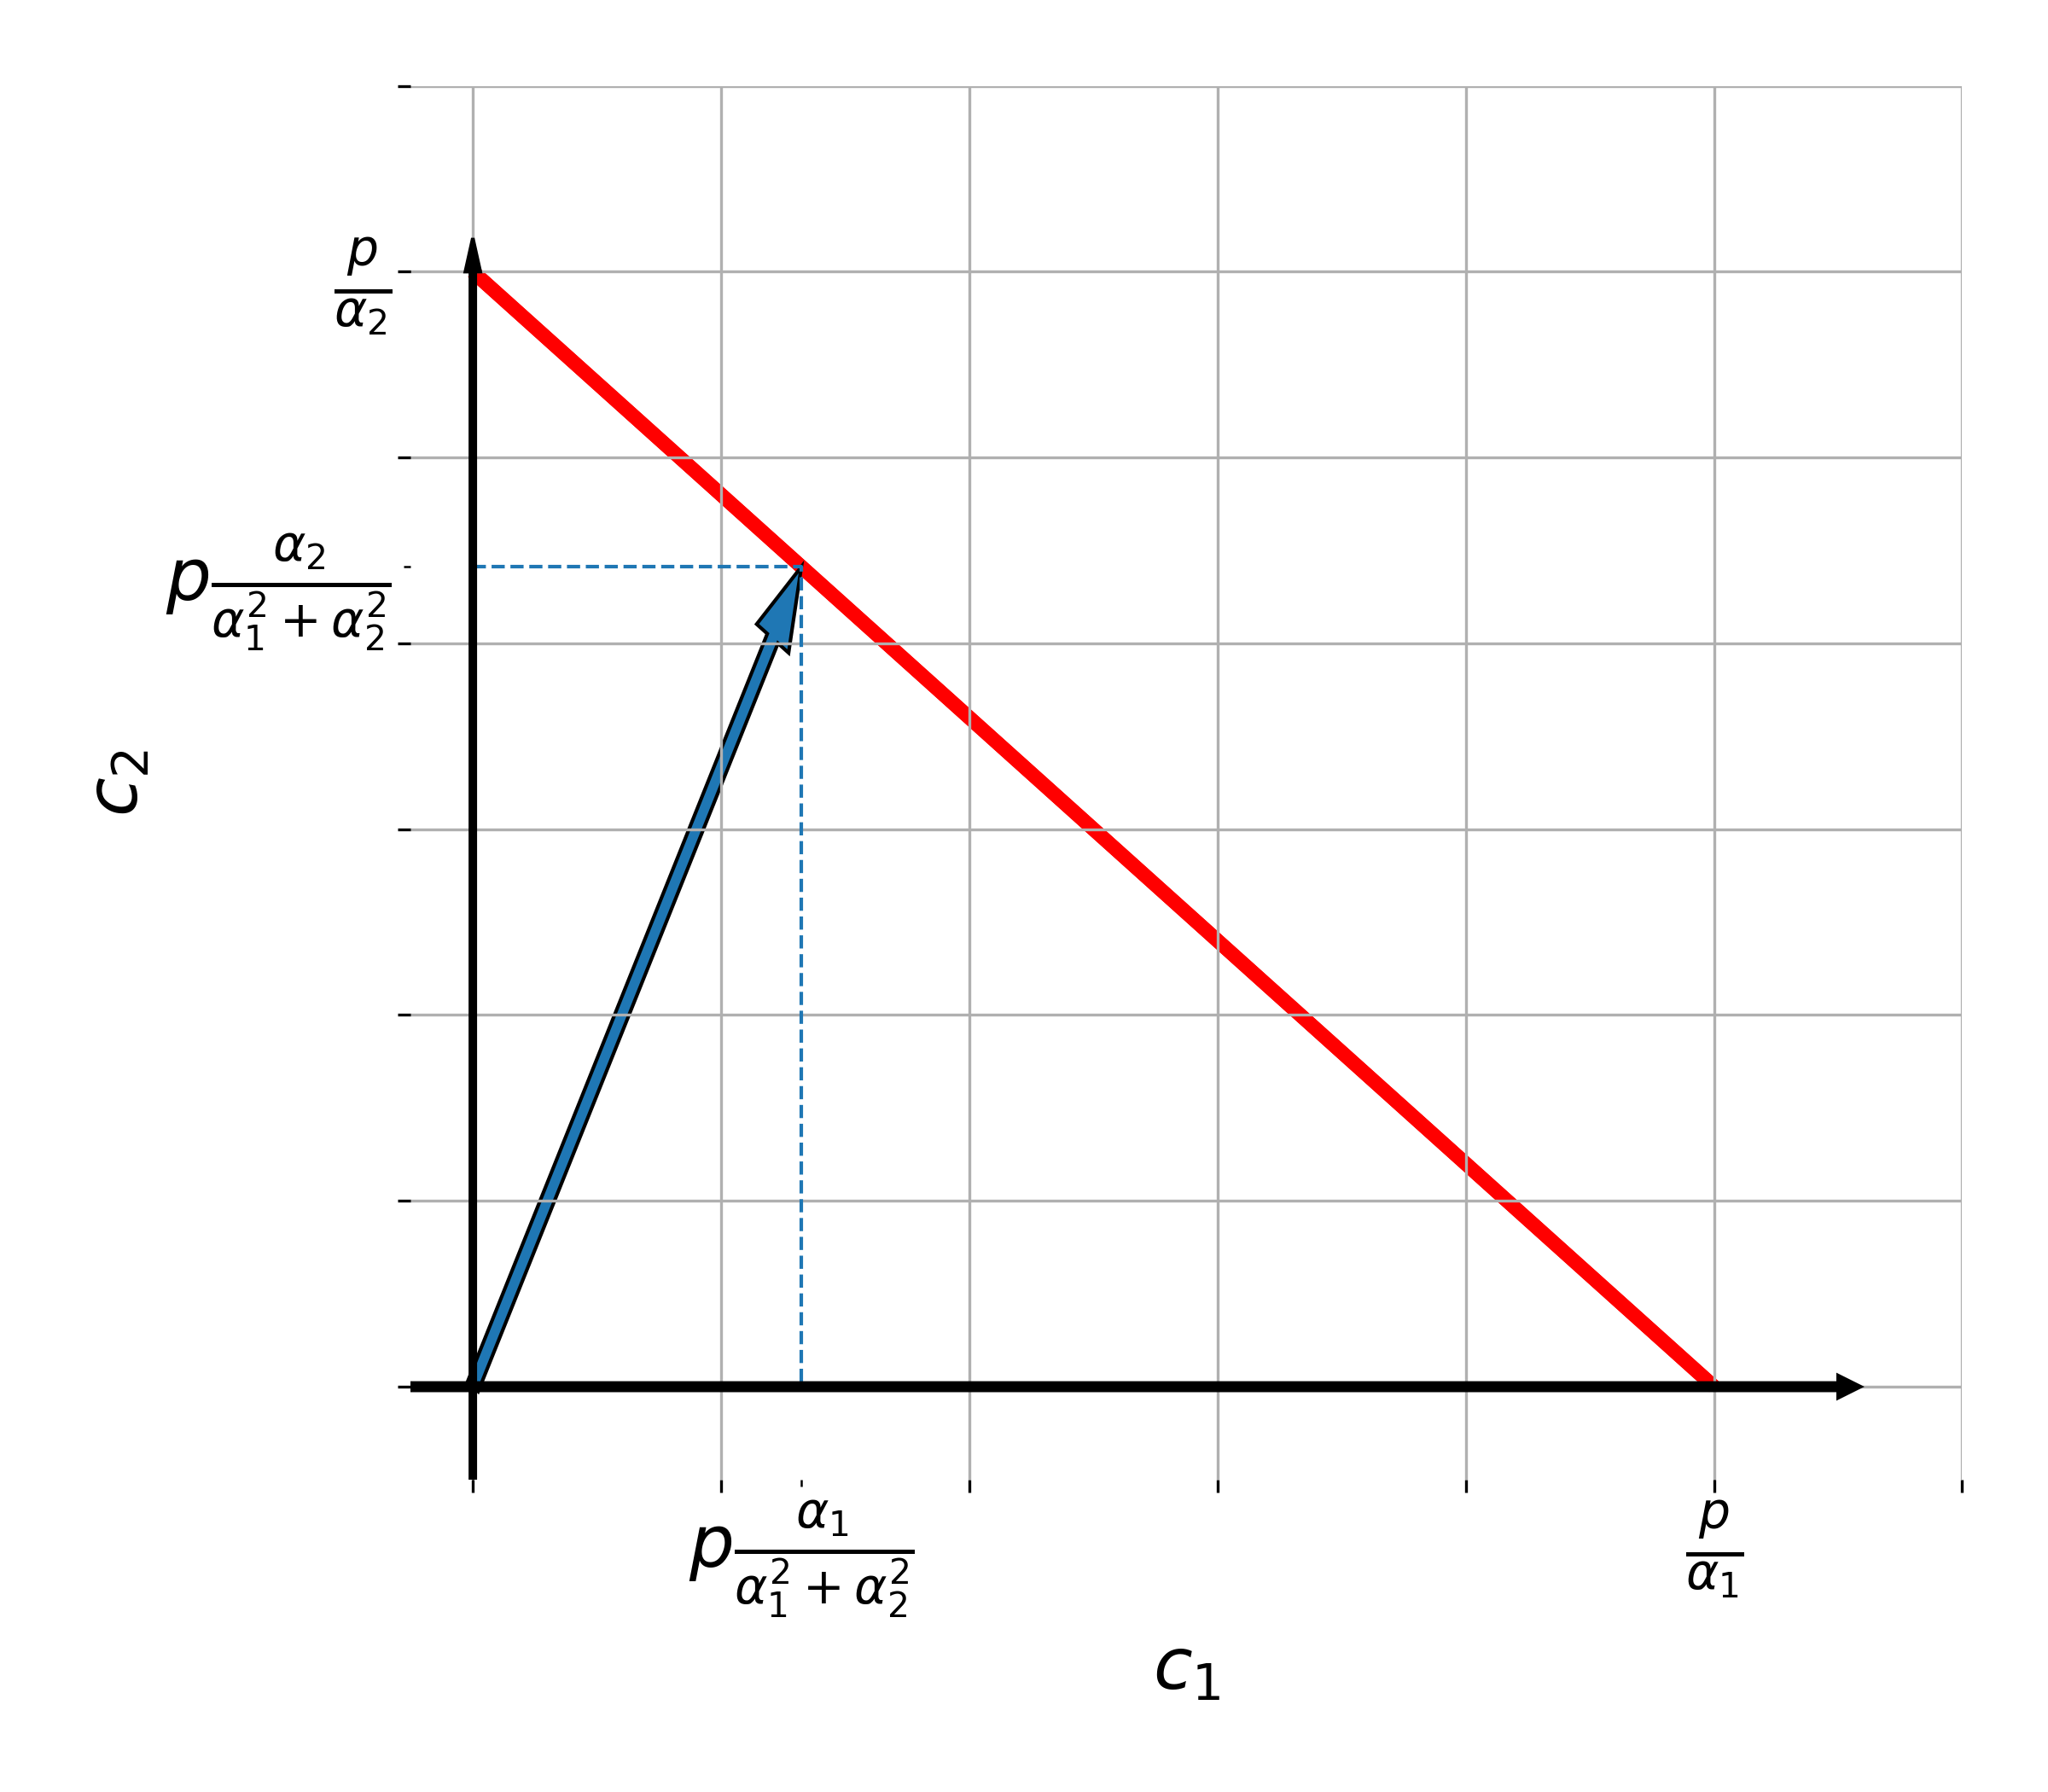
\includegraphics[width=0.8\textwidth]{part3_img/c1_c2_plot}
  \caption{Градиентная процедура минимизации не может найти истинное соотношение концентраций.}
  \label{fig:c1_c2_plot}
\end{figure}

Этот пример иллюстрирует невозможность градиентной процедурой пространствено ``разделить'' концентрации разных элементов в задаче.
Однако ситуацию можно исправить, если ввести априорное предположение о том, что в одном пикселе сканируемой площади может находиться только один элемент из смеси.
Данное условие можно сформулировать в виде уравения $c_1(x,y) * c_2(x,y) = 0 \forall x,y$ для двух элементов.
Введя операцию поэлементного умножения векторв $(\cdot \odot \cdot)$, и записав $\frac{K(K-1)}{2}$ ограничений для всех пар, получится $c_{k} \odot c_{s} = 0$, если $k \neq s$.

Данные ограничения-неравенства предлагается добавить в виде аддитивных квадратичных штрафов в функционал оптимизации.
Так же учтем, что концентрации принимают значения в интервале от 0 до 1 в виде ограничений-неравенств.
Финальный вид оптимизационной задачи МВН \eqref{eq:wrm_opt}:

\begin{equation}
\label{eq:wrm_opt}
  \begin{cases}
    \begin{array}{lc}
    Q(c) + \beta\sum_{k_1 != k_2}\Norm{c_{k_1} \odot c_{k_2}} \to \min \limits_c & w.r.t \\
    c_k \geq 0 & \\
    c_k \leq 1
    \end{array}
  \end{cases}.
\end{equation}

Для решения оптимизационной задачи с ограничениями-неравенствами \eqref{eq:wrm_opt} применяется метод барьерных функций \eqref{eq:quadprog_barrier}.
Для того, чтобы добиться наиболее разного поведения для переменных $c_1$ и $c_2$ применялись дополнительно следующие меры.
Во-первых, начальные значения для концентраций инициализируются семлированием пикселей из случайных обрезанных нормальных величин (truncated normal distribution).
Этот подход часто используется, например, при обучении нейронных сетей градиентными методами обратного распространения ошибки и помогает оптимизации избежать выхода на ``плато''

Другой подход для того чтобы повысить неоднородность восстановления заключался в том, чтобы с одного шага градиента обновлять не все изображение $c_k$, а лишь некоторую произвольную подобласть изображения.
Подобласть выбиралась двумя способами: мозаичным и гауссовым.
В первом изображение делилось на некоторое фиксированное число квадратных подобластей, и активная подобласть просто случайным образом выбиралась.
Это приводит к появлению мозайчатых артефактов на ``стыках'' областей.
Второй --- к плавному прибавлению градиента, ослабленного гауссовым окном со случайным центром.
Этот подход позволяет получить более мягко сглаженную картину, однако в результате все равно появляются характерные артефакты, в виде максимумов интенсивности в произвольных местах.
Более того, такие методы сильно замедляют сходимость метода, т.к. из всего вычисленного градиента используется только малая часть.

\section{Численный эксперимент}
Описанный алгоритм и регуляризации были имплементированы в рамках комплекса программ whitomo \cite{whitomo}.
Поведение алгоритма и результаты восстановления были рассмотрены на примере как синтетических фантомов, измерения которых были результатми компьютерной симуляции, так и реальных экспериментальных данных.
Все эксперименты были проведены для смеси из двух компонент.

В качестве фантомов рассматривались различные простые конфигурации из окружностей и эллипсов.
В рамках разработанного ПО реализована возможность выбора различной конфигурации а так же спектральных функций поглощения элементов, составляющих объект.
Для экспериментов с синтетическими данными использовался модельный спектр и характеристики поглощения, продемонстрированные на рис. \ref{fig:synth_spectrum}.
Спектр имеет пики на энергиях 2.5 и 10 кэВ, которые совпадают с пиками поглощения обоих элементов.

\begin{figure}
\centering
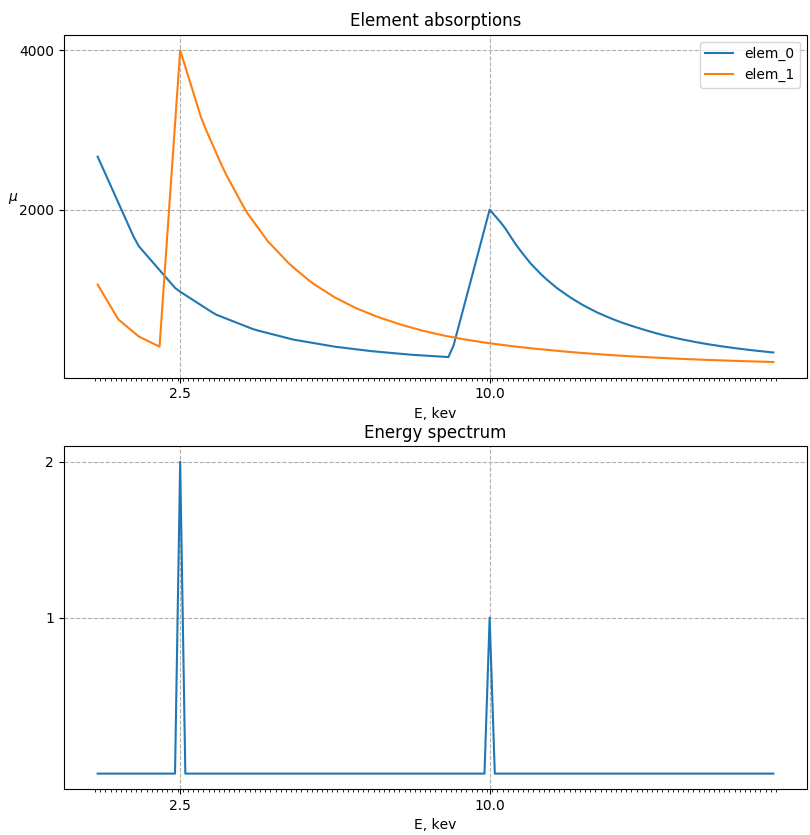
\includegraphics[height=0.5\textheight]{part3_img/synth_spectre}

\caption{Спектр зондирования и массовые коэффициенты ослабления элементов для симуляций измерений фантомов.}
\label{fig:synth_spectrum}
\end{figure}

Форма используемых фантомов и результаты восстановления методом взвешанных невязок приведены на рис. \ref{fig:synth_recon}.
Реконструкция способна пространственно разделить объекты разных элементов, т.е. восстановленные концентрации $c_1, c_2$ отличаются больше чем на константу.
Восстановленные объекты видны на картинах концентраций.
На картине концентрации слабопоглощающего элемента присутствуюты артефакты восстановления: ``тень'' от другого объекта а так же сам пик концентрации не достигает истинного значения 1.0.

\begin{figure}
\centering
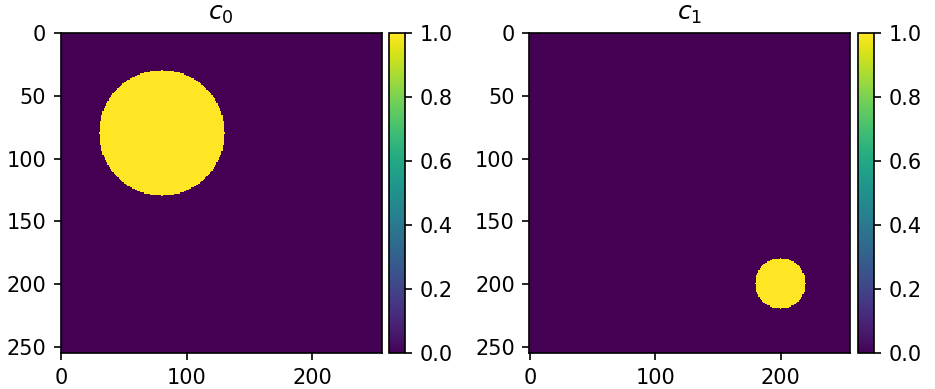
\includegraphics[width=\textwidth]{../Presentation/images/0999}
\\
a)
\\
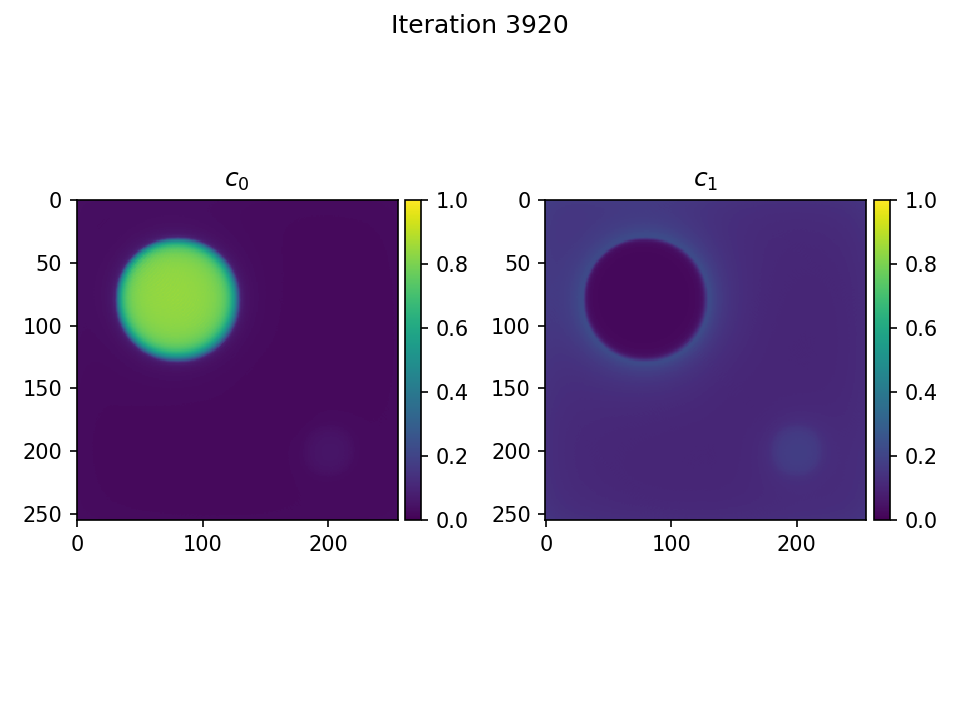
\includegraphics[width=\textwidth]{../Presentation/images/whiterec_res}
\\
б)
\\
\caption{Результаты эксперимента с синтетическими данными: а) фантом. б) восстановление}

\todo{отображение на одной картинке концентраций различных элементов}

\todo{кросс-секции вдоль диагонали}
\label{fig:synth_recon}
\end{figure}

\todo{восстановление зуба}

\todo{выводы по главе}

\todo{нормальное заключение}

\todo{побольше ссылок про полихроматику в литобзор}

\begin{comment}
\section{Численный Эксперимент} \label{sect_3_2}
Одним из результатов данной главы является программная реализация и исследование работы алгоритма восстановления, основанного на взешенных невязках.
Алгоритм был реализован на языке python с использованием библиотеки ASTRA \cite{van2015astra}.
Для восстановления были использованы различные конфигурации модельных данных, так и модельные данные (фантом), состоящий из двух овальных областей, имеющих пересечение и состоящих из элементов номер 22 и 28.
Распределения концентраций элементов представлены на рисунке \ref{fig:white_phantom}




%\begin{figure}
%\begin{subfigure}[h]{0.45\textwidth}
%  \centering
%    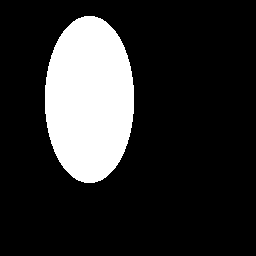
\includegraphics[width=\textwidth]{part3_img/c_22}
%  $c_22$
%\end{subfigure}
%\begin{subfigure}[h]{0.45\textwidth}
%  \centering
%    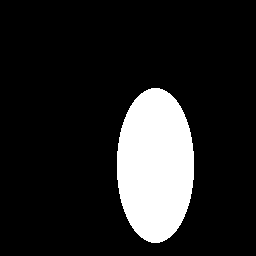
\includegraphics[width=\textwidth]{part3_img/c_28}
%  $c_28$
%\end{subfigure}
%  \caption{Используемые для симуляций концентрации}
%\label{fig:white_phantom}
%\end{figure}

\begin{figure}
  \centering
\begin{tabular}{@{}c@{}c}
    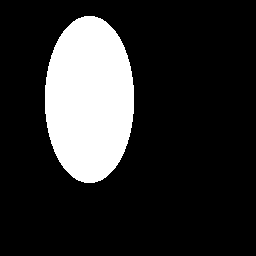
\includegraphics[width=0.45\textwidth]{part3_img/c_22}
  &
    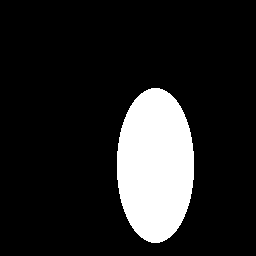
\includegraphics[width=0.45\textwidth]{part3_img/c_28}
  \\
    $c_22$ & $c_28$
\end{tabular}
  \caption{Используемые для симуляций концентрации}
\label{fig:white_phantom}
\end{figure}


На рисунке \ref{fig:source} представлены спектры поглащения элементов и спектр испускания выбранного для симуляций источника.

\begin{figure}
  \centering
  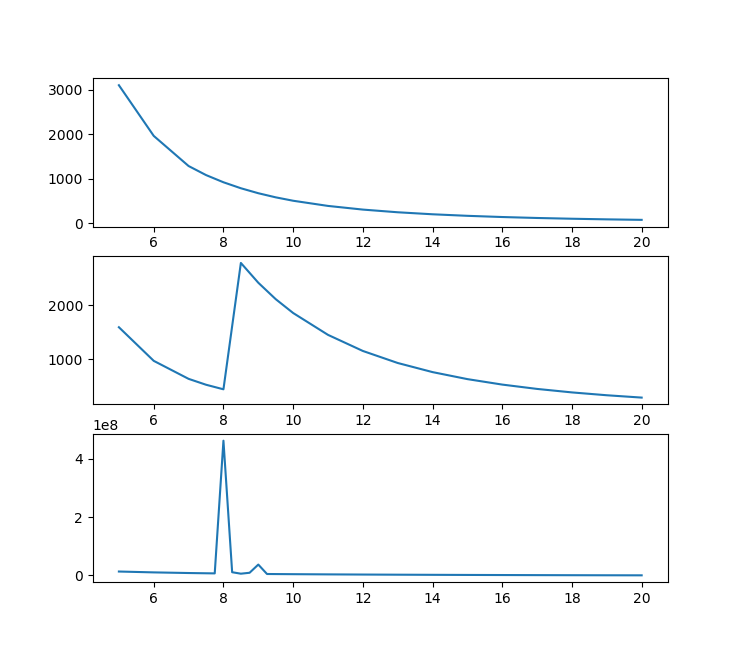
\includegraphics[width=0.95\textwidth]{part3_img/graphs}
  \caption{Сверху вниз: коэффициент поглощения для элементов 22, 28 и спект источника}
  \label{fig:source}
\end{figure}

При проведении первых симуляций оказалось, что восстановление итерационными методами сходится к локальному минмуму мультиспектральной задачи.
Это проявляется в том, что промежуточные концентрации в результате градиентного спуска приходят в вырожденному решению, не содержащему специфики элементов, из которых состоит образец.
Обе концентрации получаются равномерно размазанными по площади, занятой объектом, с характерными артефактами --- лишним увеличением концентрации вдоль выпуклой оболочки \ref{fig:wrart_noreg_25}.
Вырождение состоит в том, что значения концентраций отличаются в константу раз равномерно по всей площади восстанавливаемых концентраций.

\begin{figure}
  \centering
  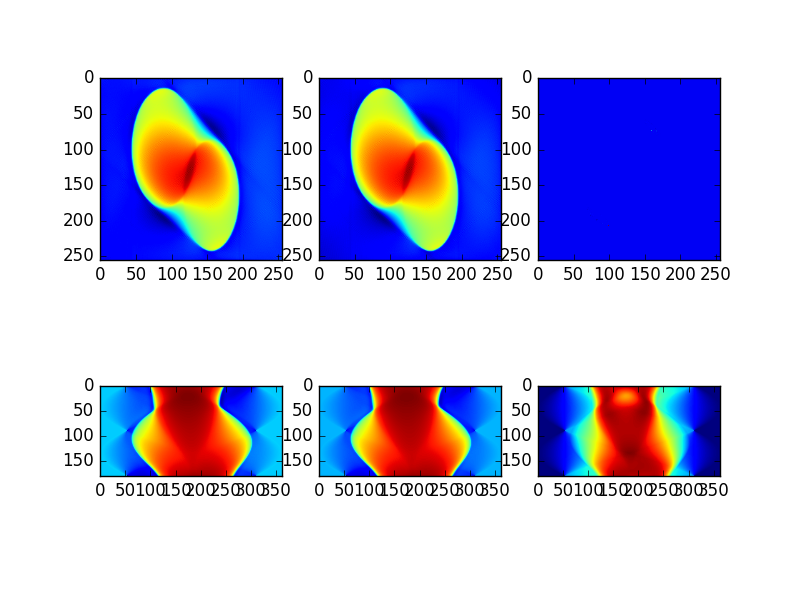
\includegraphics[width=0.95\textwidth]{part3_img/no_reg_iteration_25}
  \caption{Восстановление с помощью МВН, концентрации и их отношение, их синограммы и отношения}
  \label{fig:wrart_noreg_25}
\end{figure}

\todo{вывести соотношение, к которому выраждаются восстановленные картины}

\section{Полихроматическая регуляризация}
\todo{описать подробно регуляризацию модуля произведений}

Вырождение концентраций различных элементов легко проиллюстрировать следующим примером.

\todo{сингулярный спектр, сингулярные кривые поглащения двух элементов. реконструкция - решение уравнения с 2 неизвестными. график в координатах c1, c2, решение лежит на отрезке между осями в положительном квадранте (для некоторого пикселя). вырождение идет к прямой $c_1 = \alpha c_2$. Нужно запретить это - одновременно нельзя обеим концентрациям быть положительными. Иными словами, $c_1 c_2 = 0$}

Логичным ограничением при оптимизации является запретить находиться в одном пикселе восстанавливаемой площади концентраций двух разных элементов.
Чтобы ввести такое ограничение, можно перейти к задаче условной оптимизации, добавив ограничение $c_1 c_2 = 0$ или, в случае $K$ различных элементов $\frac{ K (K - 1) } { 2 }$ ограничений вида $c_{k_1} c_{k_2} = 0, k_1 \neq k_2$.
Так же можно добавить условия на положительность концентраций $c_k \geq 0$.
В результате восстановление томографии в полихроматической моде сведется к оптимизации с ограничениями.
Следуя логике раздела \ref{sect_2_2}, заменяя жесткие ограничения-равенства на мягкие, получаем что регуляризация может быть получена добавлением в целевую функцию штрафов за модуль произведения концентраций. 
Дополнительно добавляется мягкий штраф за отличие значений концентраций от 0 и 1, подобно тому как это сделано в \cite{svets2016}: $||c - 0.5||^2$
\todo{описать подробнее}

Результаты восстановления с использованием такой мультипликативной регуляризации (мягких ограничений-равенств условной оптимизации) представлены на рисунке \ref{fig:wrart_mulreg_150}

\begin{figure}
  \centering
  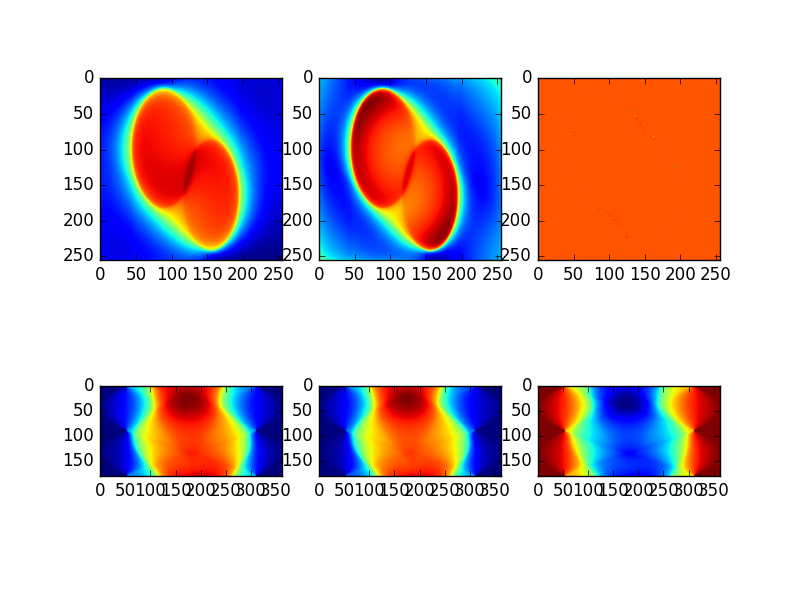
\includegraphics[width=0.95\textwidth]{part3_img/mul_reg_iteration_150}
  \caption{Восстановление с помощью МВН с использованием мультипликативной регуляризации}
  \label{fig:wrart_mulreg_150}
\end{figure}

\todo{описать переход к вырожденному спектру}

\end{comment}

\section{Выводы} \label{sect_3_3}
           % Глава 3
\chapter*{Заключение}						% Заголовок
\addcontentsline{toc}{chapter}{Заключение}	% Добавляем его в оглавление

%% Согласно ГОСТ Р 7.0.11-2011:
%% 5.3.3 В заключении диссертации излагают итоги выполненного исследования, рекомендации, перспективы дальнейшей разработки темы.
%% 9.2.3 В заключении автореферата диссертации излагают итоги данного исследования, рекомендации и перспективы дальнейшей разработки темы.
%% Поэтому имеет смысл сделать эту часть общей и загрузить из одного файла в автореферат и в диссертацию:
%% Согласно ГОСТ Р 7.0.11-2011:
%% 5.3.3 В заключении диссертации излагают итоги выполненного исследования, рекомендации, перспективы дальнейшей разработки темы.
%% 9.2.3 В заключении автореферата диссертации излагают итоги данного исследования, рекомендации и перспективы дальнейшей разработки темы.
\begin{enumerate}
  \item Получено аналитическое выражение для операции транспонированного быстрого преобразования Хафа. Доказана теорема о симметричности четверти БПХ, отвечающей одной группе ориентаций лучей. Получен метод вычислительно эффективного вычисления транспонированного преобразования.
  \item Построен вычислительно эффективный алгебраический метод восстановления измерений компьютерной томографии на основе БПХ. Произведена адаптация метода для работы с данными реальных измерений. Изучены свойства пространства БПХ, влияние различной регуляризации на процесс восстановления.
  \item Построен метод восстановления рентгеновской томографии методом квадратичного программирования для объектов, содержащих сильнопоглощающие включения. На реальных экспериментальных измерениях проведено исследование метода мягких ограничений \todo{и сравнение с методом квадратичного программирования}
  \item Построен алгебраический алгоритм восстановления томографии в задаче зондирования полихроматическим излучением, основанный на вычиследнии взвешанных невязок по каждому из элементов, входящих в состав исследуемого образца. Предложены варианты регуляризации для востановления в полихроматической моде. \todo{описать, какой получен результат}
\end{enumerate}
      % Заключение
\chapter*{Список сокращений и условных обозначений}
\begin{itemize}
\item КТ --- Компьютерная томография
\item ART --- Algebraic Reconstruction Technique, Алгебраический Метод Восстановления
\item FBP --- Filtered Backprojection, метод свертки и обратной проекции
\item ПО --- Программное Обеспечение
\item FHT --- fast Hough transform
\item БПХ --- быстрое преобразование Хафа
\item МВН --- метод взвешанных невязок
\end{itemize}        % Список сокращений и условных обозначений
\chapter*{Словарь терминов}             % Заголовок
\addcontentsline{toc}{chapter}{Словарь терминов}  % Добавляем его в оглавление

\textbf{синограмма} - входные данные для алгоритмов восстановления компьютерной томографии
      % Словарь терминов
\clearpage                                  % В том числе гарантирует, что список литературы в оглавлении будет с правильным номером страницы
%\hypersetup{ urlcolor=black }               % Ссылки делаем чёрными
%\providecommand*{\BibDash}{}                % В стилях ugost2008 отключаем использование тире как разделителя 
\urlstyle{rm}                               % ссылки URL обычным шрифтом
\ifdefmacro{\microtypesetup}{\microtypesetup{protrusion=false}}{} % не рекомендуется применять пакет микротипографики к автоматически генерируемому списку литературы
\insertbibliofull                           % Подключаем Bib-базы
\ifdefmacro{\microtypesetup}{\microtypesetup{protrusion=true}}{}
\urlstyle{tt}                               % возвращаем установки шрифта ссылок URL
%\hypersetup{ urlcolor={urlcolor} }          % Восстанавливаем цвет ссылок      % Список литературы
\clearpage
\ifdefmacro{\microtypesetup}{\microtypesetup{protrusion=false}}{} % не рекомендуется применять пакет микротипографики к автоматически генерируемым спискам
\listoffigures  % Список изображений

%%% Список таблиц %%%
% (ГОСТ Р 7.0.11-2011, 5.3.10)
\clearpage
\listoftables   % Список таблиц
\ifdefmacro{\microtypesetup}{\microtypesetup{protrusion=true}}{}
\newpage           % Списки таблиц и изображений (иллюстративный материал)
\input{Dissertation/appendixsetup}   % Предварительные настройки для правильного подключения Приложений
        % Приложения

\end{document}
